\documentclass[a4paper,12pt,twoside]{article}
\usepackage{amsmath}
\usepackage{amssymb}
\usepackage{bm}
\usepackage{booktabs}
\usepackage[small,bf]{caption}
\usepackage{comment}
\usepackage{cuted}
\usepackage[shortlabels]{enumitem}
\usepackage{fancyhdr}
\usepackage{fancybox}
\usepackage{float}
\usepackage[T1]{fontenc}
\usepackage[a4paper,left=1in,right=1in,top=0.25in,bottom=1in,
    headheight=76.33466pt,
    headsep=\dimexpr1in-62.33466pt\relax,
    includehead
]{geometry}
\usepackage{graphicx}
\usepackage{hyperref}
\usepackage[utf8]{inputenc}
% \usepackage{lipsum}
\usepackage{listings}
\usepackage{minted}
\usemintedstyle{emacs}
\usepackage{multirow}
\usepackage{parskip}
\usepackage{ragged2e}
\usepackage{setspace}
\usepackage{soul}
% \onehalfspacing
\usepackage{subcaption}
% \usepackage[subrefformat=parens,labelformat=parens]{subfig}
\usepackage{tabularx}
% \usepackage{titling}
\usepackage{xurl}
\usepackage{biblatex}
\addbibresource{Lab6.bib}
\usepackage{background}
\backgroundsetup{contents=
\includegraphics{waterprint.jpg}, scale=0.8, opacity=0.1}
\pagestyle{fancy}
\fancyhf{}
\fancyhead[LE,RO]{}
\fancyhead[CE,CO]{
\includegraphics[width=0.7\textwidth]{JILogo.png}}
\fancyhead[RE,LO]{}
\fancyfoot[CE,CO]{\leftmark}
\fancyfoot[CE,CO]{\thepage}
\lfoot{\textit{ECE4810J \textbf{SoC Design} | Fall 2022}}
\renewcommand{\headrulewidth}{1pt}
\renewcommand{\footrulewidth}{1pt}
\definecolor{caption2color}{HTML}{2e5395}
\hypersetup{
    colorlinks=true,
    linkcolor=blue,
    filecolor=magenta,      
    urlcolor=cyan,
    pdfpagemode=FullScreen,
}
\definecolor{codegreen}{rgb}{0,0.6,0}
\definecolor{codegray}{rgb}{0.5,0.5,0.5}
\definecolor{codepurple}{rgb}{0.58,0,0.82}
\definecolor{backcolour}{rgb}{0.95,0.95,0.92}

\lstdefinestyle{mystyle}{
    backgroundcolor=\color{backcolour},   
    commentstyle=\color{codegreen},
    keywordstyle=\color{magenta},
    numberstyle=\tiny\color{codegray},
    stringstyle=\color{codepurple},
    basicstyle=\ttfamily\footnotesize,
    breakatwhitespace=false,         
    breaklines=true,                 
    captionpos=b,                    
    keepspaces=true,                 
    numbers=left,                    
    numbersep=5pt,                  
    showspaces=false,                
    showstringspaces=false,
    showtabs=false,                  
    tabsize=2
}

\lstset{style=mystyle}

\usepackage[percent]{overpic}

\author{Yihua Liu}
\title{ECE4810J FA2021\\ \small Lab \#4}
\date{October 24, 2022}

\begin{document}
% \maketitle
\thispagestyle{fancy}

\begin{center}
    \vspace*{0pt}
    \Large{\textbf{ECE4810J SoC Design}}\\
    \vspace*{2pt}
    \large{Fall 2022}\\
    \vspace*{10pt}
    \Large{\textcolor{caption2color}{Lab \#6 Automated ASIC Block Flow}}\\
    \normalsize{\hl{Due: 11:59pm Nov. 13th, 2022}}
    \rule[-5pt]{.97\linewidth}{0.05em}
\end{center}

\textbf{Logistics:}
\begin{itemize}
    \item This lab is a team exercise.
    \item Please use the discussion board on Piazza for Q\&A.
    \item All reports and code (if available) MUST be submitted to the assignment of Canvas.
    \item Internet usage is allowed and encouraged.
    \item No late submission is allowed for this lab.
\end{itemize}

\tableofcontents

\newpage
\section{Overview}
In this lab, you will learn about ASIC design flow. The goals of this lab are to:
\begin{itemize}
    \item Learn OpenROAD-flow-scripts.
    \item Learn the automated ASIC block flow.
\end{itemize}

\section{OpenROAD}\label{SOR}
\subsection{Introduction}
The \href{https://theopenroadproject.org/}{OpenROAD} Project was founded in 2018 under the DARPA IDEA program to address the issue of hardware design requiring too much effort, cost, and time. Since then, the project has shown great success in providing a free, open-source implementation for ASIC designs in technology nodes as small as 7nm. Notably, OpenROAD has enabled first-time chip designers, hobbyists, and students to fabricate chips through the \href{https://efabless.com/open_shuttle_program}{Google/Efabless/Skywater 130nm free shuttle program}. Over 100 designs have been silicon-tested on the first two shuttle runs, and \href{https://opensource.googleblog.com/2022/07/SkyWater-and-Google-expand-open-source-program-to-new-90nm-technology.html}{hundreds more have been taped out} \cite{ajayi2019openroad} \cite{ajayi2019toward}.

OpenROAD provides a tremendous opportunity for researchers to perform design space exploration, collaborate, and construct real chips in a free and open-source manner. This lab will aim to:
\begin{itemize}
    \item Introduce researchers to implementation tools, specifically the \href{https://github.com/The-OpenROAD-Project/OpenROAD-flow-scripts}{OpenROAD flow toolchain}
    \item Motivate the use of open-source designs, tools, and platform development kits (PDKs) in research and teaching
    \item Provide a demonstration of OpenROAD’s features and example uses for both computer architecture research and teaching
    \item Demonstrate a clear path for attendees to turn their RTL designs into silicon through commercial fabs or the free Google/Efabless/Skywater 130nm Shuttle
\end{itemize}
\subsection{Goals}
This lab will cover using OpenROAD for both cutting-edge nodes (e.g., ASAP 7nm) and older nodes (e.g., Skywater 130nm).

In this lab, we will present:
\begin{itemize}
    \item What is an implementation flow?
    \begin{itemize}
        \item How does a design get from register-transfer level (RTL) code to a real chip?
        \item What is The OpenROAD Project?
        \item What are the benefits of open-source hardware flows?
    \end{itemize}
    \item How do I use OpenROAD?
    \begin{itemize}
        \item How do I generate a chip from my RTL or example RTL?
        \item How do I debug common design problems?
        \item How can I collect design data such as power, frequency, and area?
        \item How can I model complex designs?
    \end{itemize}
    \item What are OpenROAD’s limitations?
    \item What is OpenROAD’s roadmap?
    \item How can I contribute to OpenROAD?
\end{itemize}
This lab is intended to introduce ASIC implementation to those already conceptually familiar with RTL design. We do not cover RTL design techniques or RTL validation.

\subsection{Toolchain Installation}
Following \cite{openroadinstall}, run
\begin{minted}[breaklines,breakanywhere]{bash}
git clone --recursive https://github.com/The-OpenROAD-Project/OpenROAD-flow-scripts
cd OpenROAD-flow-scripts
./build_openroad.sh
\end{minted}
If you failed to clone, please read Appendix: Troubleshooting \ref{ATGit}. If your build failed with errors, please read Appendix: Troubleshooting \ref{ATBuild}.

After the Docker image is prepared, open \texttt{flow/scripts/report\_metrics.tcl} and comment Line 24 - 25:
\begin{minted}{tcl}
    # report_clock_skew_metric
    # report_clock_skew_metric -hold
\end{minted}
\textit{If you use WSL 2 Docker, you must start the Docker Desktop in Windows}.

Then, run
\begin{minted}[breaklines,breakanywhere]{bash}
docker run -it -u $(id -u ${USER}):$(id -g ${USER}) -v $(pwd)/flow/platforms:/OpenROAD-flow-scripts/flow/platforms:ro openroad/flow-scripts
cd /OpenROAD-flow-scripts/flow
source ./setup_env.sh
\end{minted}
Note that \texttt{setup\_env.sh} is only for running in Docker. Then, you can test tools like \texttt{yosys}, \texttt{klayout}, and \texttt{openroad}. You need an X server like \texttt{VcXsrv} or Moba X Server to show the X11 forwarded window in WSL. Pay attention to what shell you are using when running commands. If the prompt begins with \texttt{bash-4.2\$}, then it is Bash; if the prompt begins with \texttt{\%}, then it is Tcl shell. Under \texttt{/OpenROAD-flow-scripts/flow}, in Bash, run
\begin{minted}{bash}
make
\end{minted}
If the flow completes without error, congrats! You are ready to start the lab. You should run \texttt{make clean\_all} to reset your flow build.

The OpenROAD Project uses three tools to perform automated RTL-to-GDS layout generation:
\begin{itemize}
    \item \href{https://github.com/The-OpenROAD-Project/yosys}{yosys}: Logic Synthesis
    \item \href{https://github.com/The-OpenROAD-Project/OpenROAD}{OpenROAD App}: Floorplanning through Detailed Routing
    \item \href{https://www.klayout.de/}{KLayout}: GDS merge, DRC and LVS (public PDKs)
\end{itemize}
To automate RTL-to-GDS, \href{https://github.com/The-OpenROAD-Project/OpenROAD-flow-scripts}{OpenROAD Flow} is provided, which contains scripts that integrate the three tools. The OpenROAD Flow repository serves as an example of RTL-to-GDS flow using the OpenROAD tools. The script build\_openroad.sh in the repository will automatically build the OpenROAD toolchain. The two main directories are:
\begin{enumerate}
    \item \texttt{tools/}: contains the source code for the entire \texttt{yosys} and \href{https://github.com/The-OpenROAD-Project/OpenROAD}{OpenROAD App} (both via submodules) as well as other tools required for the flow.
    \item \texttt{flow/}: contains reference recipes and scripts to run designs through the flow. It also contains public platforms and test designs.
\end{enumerate}
\subsection{X11 in WSL Docker}
If you use WSL 2, the \texttt{DISPLAY} variable is set to ":0" by default, and it can directly connect to the X Server in your Windows (\textit{you must start your X server in Windows first}). However, to connect in Docker in WSL, there is a little bit more thing to do \cite{wsldockerx11}.
\begin{enumerate}
    \item In Windows Command Prompt or PowerShell, run \texttt{ipconfig}.
    \item Find the item "Ethernet adapter vEthernet (WSL)".
    \item Find the IPv4 Address of "Ethernet adapter vEthernet (WSL)", for example, 172.22.48.1.
    \item In WSL 2, run Docker with the given options.
    \item In Docker in WSL, run
    \begin{minted}{bash}
export DISPLAY=172.22.48.1:0.0
    \end{minted}
    \item Run a GUI app to test whether the X11 is set up. You can alternatively pass the DISPLAY variable by the \texttt{-e} option of \texttt{docker run}.
\end{enumerate}
You can ignore the errors:
\begin{minted}[breaklines,breakanywhere]{text}
QStandardPaths: XDG_RUNTIME_DIR not set, defaulting to '/tmp/runtime-'
xkbcommon: ERROR: failed to add default include path /usr/share/X11/xkb
Qt: Failed to create XKB context!
Use QT_XKB_CONFIG_ROOT environmental variable to provide an additional search path, add ':' as separator to provide several search paths and/or make sure that XKB configuration data directory contains recent enough contents, to update please see http://cgit.freedesktop.org/xkeyboard-config/ .
libGL error: unable to load driver: swrast_dri.so
libGL error: failed to load driver: swrast
\end{minted}
To access the files in WSL, you can use the \texttt{-v} option of \texttt{docker run}. You can bind mount multiple volumes by passing two \texttt{-v} arguments, for example,
\begin{minted}[breaklines,breakanywhere]{bash}
docker run -it -u $(id -u ${USER}):$(id -g ${USER}) -net=host -v $(pwd)/flow/platforms:/OpenROAD-flow-scripts/flow/platforms:ro /mnt/f/Documents/Master/TA/Resources/exercises:/exercises openroad/flow-scripts
\end{minted}

\subsection{Running the Flow}\label{SRF}
\subsubsection{Synthesis}
Run \texttt{make synth} and examine the output:
\begin{enumerate}
    \item Perform file preprocessing (mainly for \texttt{yosys})
    \begin{minted}[breaklines,breakanywhere]{text}
[INFO][FLOW] Using platform directory ./platforms/nangate45
./util/markDontUse.py -p "TAPCELL_X1 FILLCELL_X1 AOI211_X1 OAI211_X1" -i platforms/nangate45/lib/NangateOpenCellLibrary_typical.lib -o objects/nangate45/gcd/base/lib/NangateOpenCellLibrary_typical.lib
Opening file for replace: platforms/nangate45/lib/NangateOpenCellLibrary_typical.lib
Marked 4 cells as dont_use
Commented 0 lines containing "original_pin"
Replaced malformed functions 0
Writing replaced file: objects/nangate45/gcd/base/lib/NangateOpenCellLibrary_typical.lib
mkdir -p ./results/nangate45/gcd/base ./logs/nangate45/gcd/base ./reports/nangate45/gcd/base
(/usr/bin/time -f 'Elapsed time: %E[h:]min:sec. CPU time: user %U sys %S (%P). Peak memory: %MKB.' /OpenROAD-flow-scripts/tools/install/yosys/bin/yosys -v 3 -c ./scripts/synth.tcl) 2>&1 | tee ./logs/nangate45/gcd/base/1_1_yosys.log
    \end{minted}
    \item Parse input files
    \begin{minted}[breaklines,breakanywhere]{text}
1. Executing Verilog-2005 frontend: ./designs/src/gcd/gcd.v
2. Executing Liberty frontend.
3. Executing Verilog-2005 frontend: ./platforms/nangate45/cells_clkgate.v
    \end{minted}
    \item Elaborate the design
    \begin{minted}[breaklines,breakanywhere]{text}
4. Executing SYNTH pass.
4.1. Executing HIERARCHY pass (managing design hierarchy).
4.2. Executing AST frontend in derive mode using pre-parsed AST for module `\gcd'.
...
4.3. Executing PROC pass (convert processes to netlists).
...
    \end{minted}
    \item Optimize the netlist
    \begin{minted}[breaklines,breakanywhere]{text}
4.4. Executing FLATTEN pass (flatten design).
4.5. Executing OPT_EXPR pass (perform const folding).
4.6. Executing OPT_CLEAN pass (remove unused cells and wires).
4.7. Executing CHECK pass (checking for obvious problems).
4.8. Executing OPT pass (performing simple optimizations).
...
    \end{minted}
    \item Map the generic netlist cells to technology-specific cells
    \begin{minted}[breaklines,breakanywhere]{text}
4.22. Executing TECHMAP pass (map to technology primitives).
...
6. Executing TECHMAP pass (map to technology primitives).
...
9. Executing ABC pass (technology mapping using ABC).
    \end{minted}
\end{enumerate}
\subsubsection{Floorplanning}
Run \texttt{make floorplan} and examine the output:
\begin{enumerate}
    \item Initialize chip area
    \begin{minted}[breaklines,breakanywhere]{text}
[INFO IFP-0001] Added 35 rows of 263 sites.
    \end{minted}
    \item I/O pin placement
    \begin{minted}{text}
Using 1u default distance from corners.
Using 2 tracks default min distance between IO pins.
[INFO PPL-0007] Random pin placement.
    \end{minted}
    \item Insert tapcells and endcaps
    \begin{minted}{text}
[INFO TAP-0004] Inserted 70 endcaps.
[INFO TAP-0005] Inserted 0 tapcells.
    \end{minted}
    \item Generate power grid
    \begin{minted}{text}
[INFO PDN-0001] Inserting grid: grid
    \end{minted}
\end{enumerate}
See this step in the GUI:
\begin{minted}{text}
make gui_floorplan
\end{minted}
\begin{figure}[H]
    \centering
    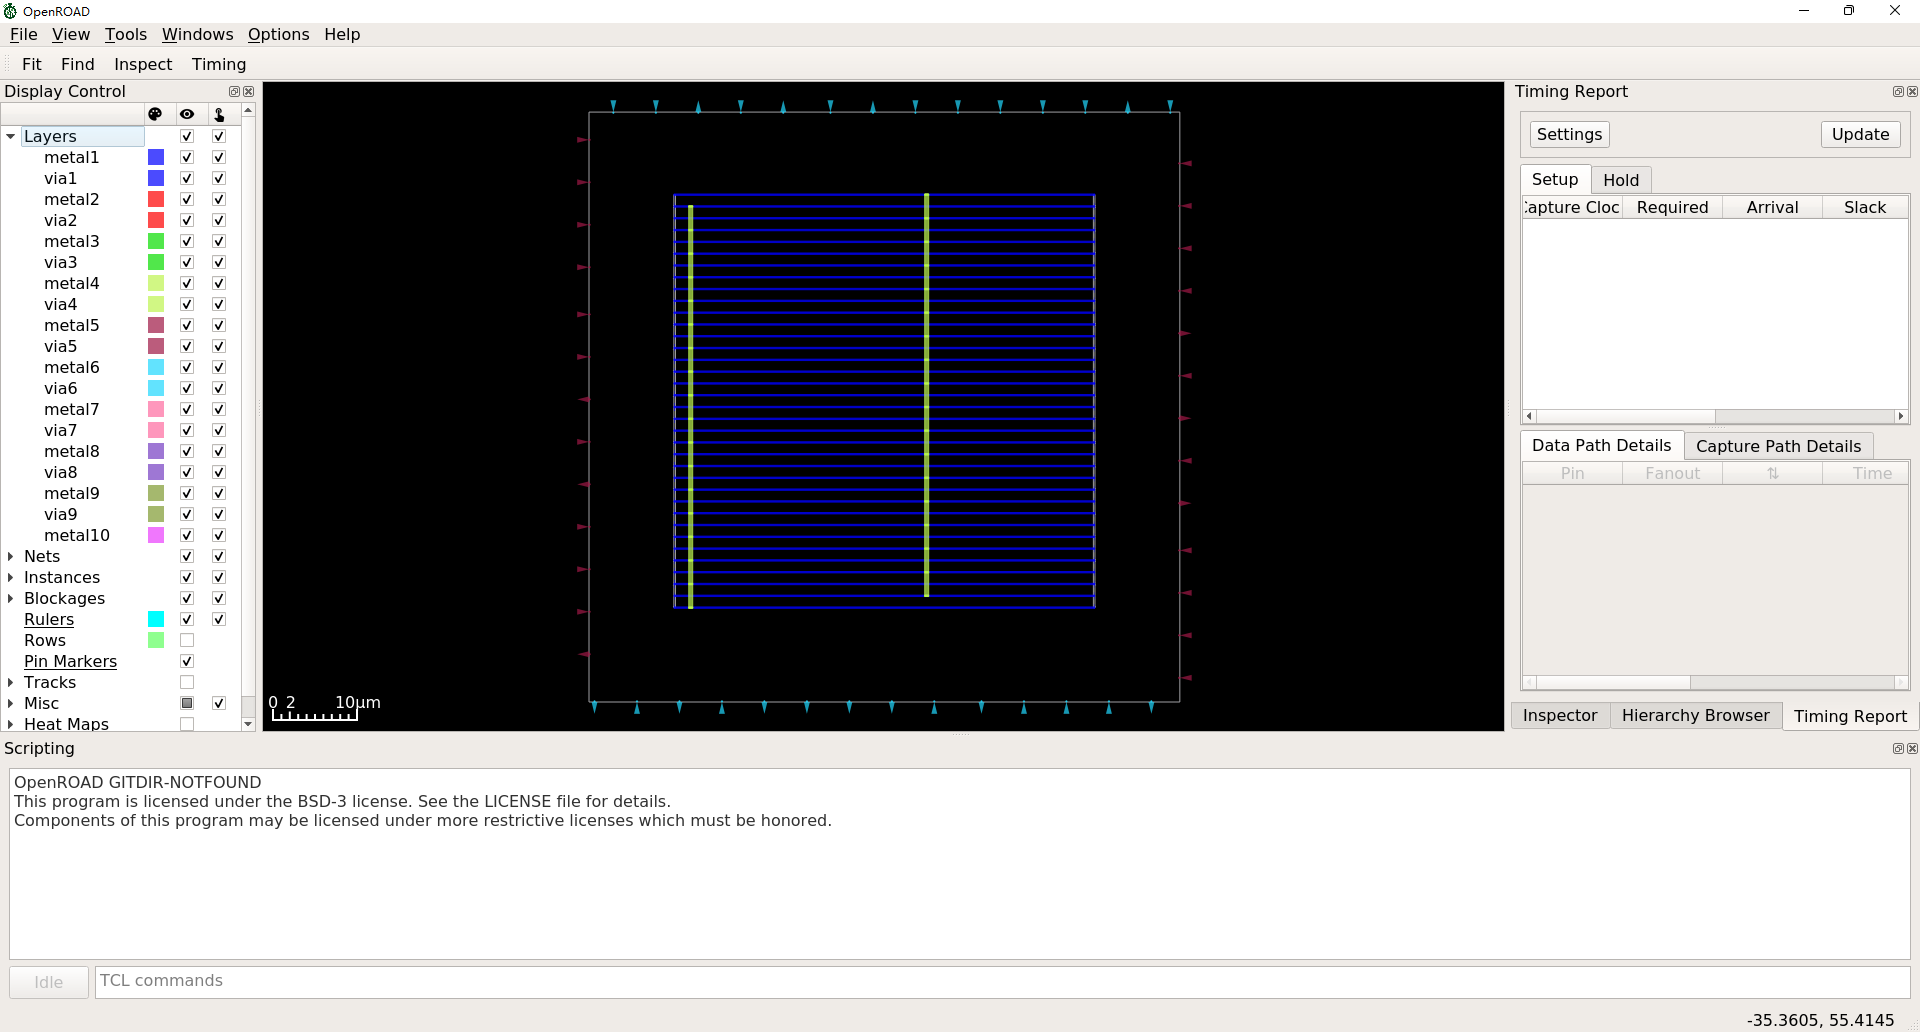
\includegraphics[width=\textwidth]{images/1.png}
\end{figure}
\subsubsection{Global Placement}
Run \texttt{make place} and examine the output:
\begin{enumerate}
    \item Initial place
    \begin{minted}{text}
[InitialPlace]  Iter: 1 CG residual: 0.00000008 HPWL: 7431482
[InitialPlace]  Iter: 2 CG residual: 0.00000011 HPWL: 6812877
[InitialPlace]  Iter: 3 CG residual: 0.00000010 HPWL: 6783199
[InitialPlace]  Iter: 4 CG residual: 0.00000010 HPWL: 6764779
[InitialPlace]  Iter: 5 CG residual: 0.00000009 HPWL: 6733515
    \end{minted}
    \item Nesterov gradient descent (with timing-driven weighting)
    \begin{minted}{text}
[NesterovSolve] Iter: 10 overflow: 0.424423 HPWL: 5509684
[NesterovSolve] Iter: 20 overflow: 0.372513 HPWL: 5236909
[NesterovSolve] Iter: 30 overflow: 0.366609 HPWL: 5245895
[NesterovSolve] Iter: 40 overflow: 0.372344 HPWL: 5230034
[NesterovSolve] Iter: 50 overflow: 0.379915 HPWL: 5258285
...
[INFO GPL-0100] worst slack -6.41e-11
[INFO GPL-0103] Weighted 38 nets.
...
[NesterovSolve] Iter: 340 overflow: 0.108812 HPWL: 5253966
[NesterovSolve] Finished with Overflow: 0.099573
    \end{minted}
    \item Timing optimization and electrical rule fixing
    \begin{minted}{text}
Perform port buffering...
[INFO RSZ-0027] Inserted 35 input buffers.
[INFO RSZ-0028] Inserted 18 output buffers.
Perform buffer insertion...
[INFO RSZ-0058] Using max wire length 661um.
[INFO RSZ-0039] Resized 39 instances.
Repair tie lo fanout...
Repair tie hi fanout...
    \end{minted}
\end{enumerate}
\subsubsection{Detailed Placement}
\begin{enumerate}
    \item Optimize and legalize placement
    \begin{minted}[breaklines]{text}
Detailed placement improvement.
Importing netlist into detailed improver.
[INFO DPO-0100] Creating network with 470 cells, 54 terminals, 471 edges and 1293 pins.
[INFO DPO-0109] Network stats: inst 524, edges 471, pins 1293
[INFO DPO-0110] Number of regions is 1
[INFO DPO-0401] Setting random seed to 1.
...
Detailed Improvement Results
------------------------------------------
Original HPWL             2885.1 u
Final HPWL                2684.2 u
Delta HPWL                  -7.0 %
    \end{minted}
    \item Cell mirroring
    \begin{minted}{text}
[INFO DPL-0020] Mirrored 14 instances
[INFO DPL-0021] HPWL before            2684.2 u
[INFO DPL-0022] HPWL after             2681.9 u
[INFO DPL-0023] HPWL delta               -0.1 %
    \end{minted}
\end{enumerate}
See this step in the GUI:
\begin{minted}{bash}
make gui_place
\end{minted}
\begin{figure}[H]
    \centering
    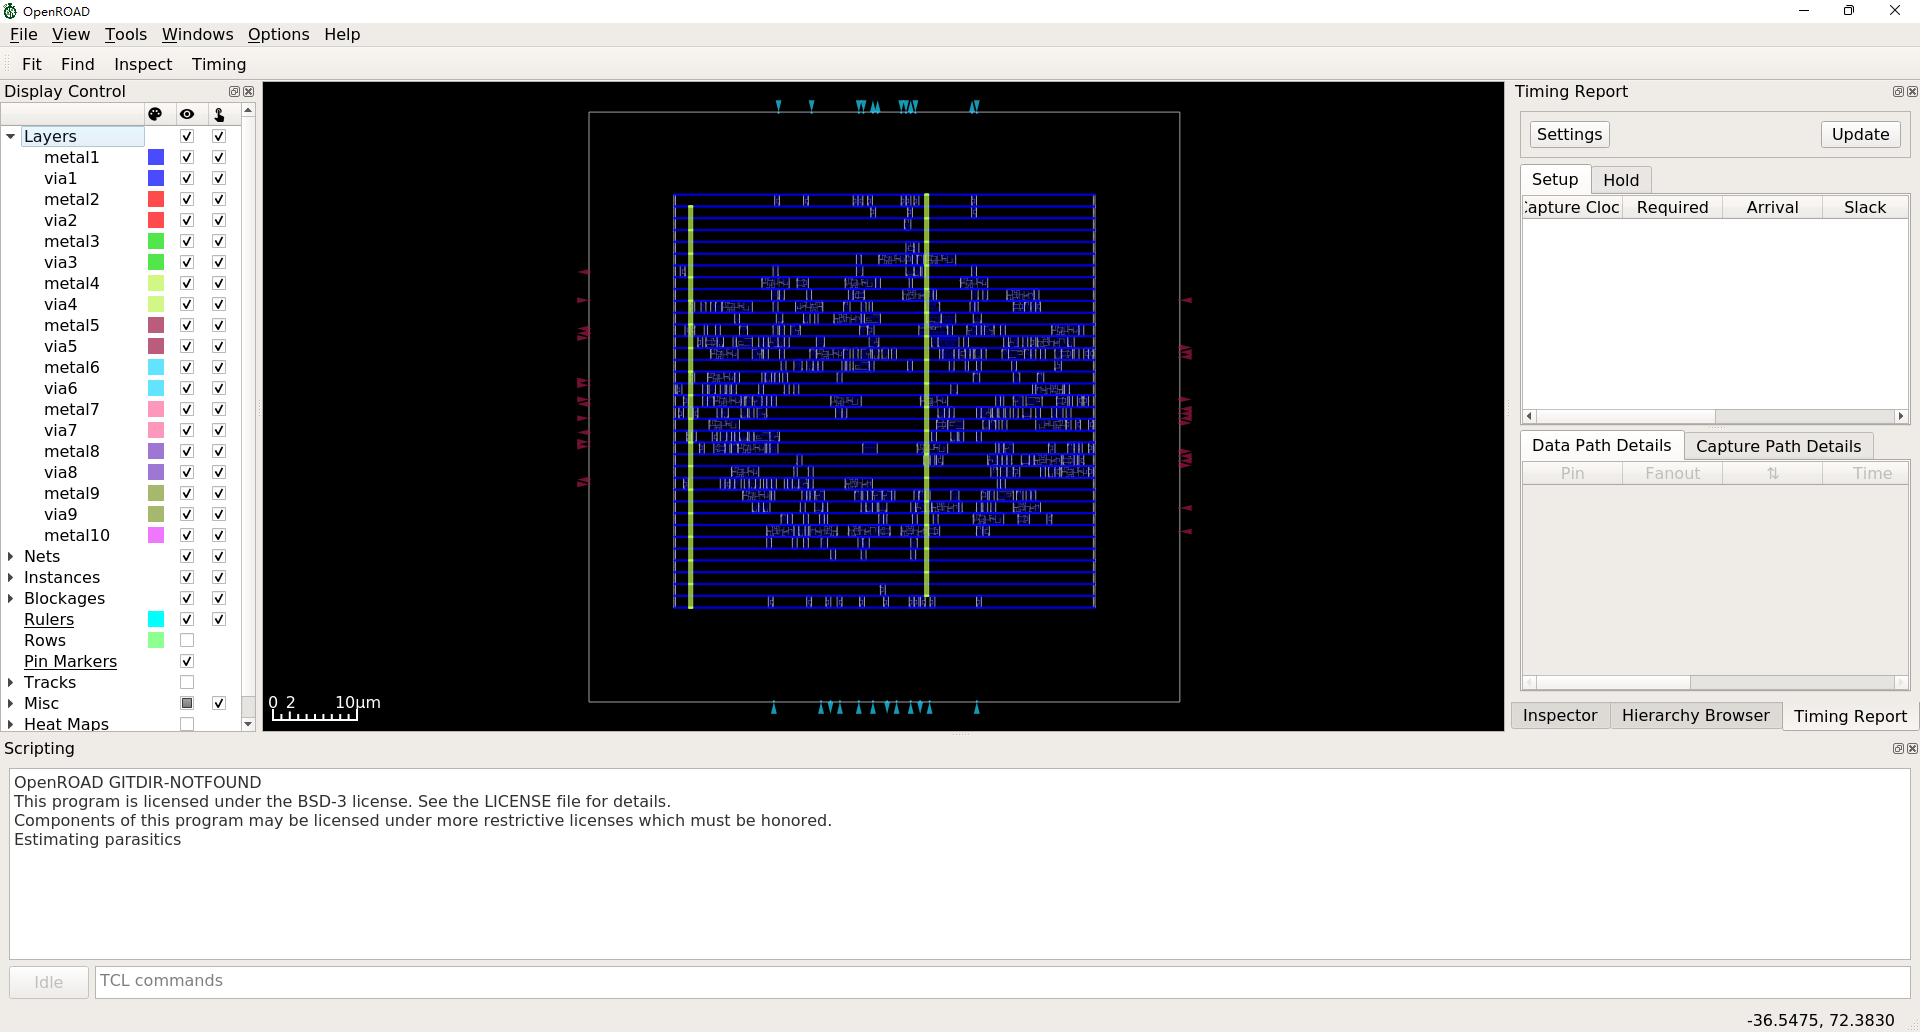
\includegraphics[width=\textwidth]{images/2.png}
\end{figure}
\subsubsection{Clock Tree Synthesis}
Run \texttt{make cts} and examine the output:
\begin{enumerate}
    \item Buffer characterization
    \begin{minted}{text}
[INFO CTS-0049] Characterization buffer is: BUF_X4.
[INFO CTS-0039] Number of created patterns = 11880.
[INFO CTS-0084] Compiling LUT.
Min. len    Max. len    Min. cap    Max. cap    Min. slew   Max. slew
2           8           1           34          1           14
    \end{minted}
    \item Generate the clock tree
    \begin{minted}{text}
[INFO CTS-0007] Net "clk" found for clock "core_clock".
[INFO CTS-0010]  Clock net "clk" has 35 sinks.
[INFO CTS-0008] TritonCTS found 1 clock nets.
[INFO CTS-0097] Characterization used 1 buffer(s) types.
[INFO CTS-0027] Generating H-Tree topology for net clk.
[INFO CTS-0028]  Total number of sinks: 35.
    \end{minted}
    \item Resize / repair clock tree
    \begin{minted}{text}
[INFO RSZ-0058] Using max wire length 661um.
    \end{minted}
    \item Legalize buffers
    \begin{minted}{text}
Placement Analysis
---------------------------------
total displacement          3.7 u
average displacement        0.0 u
max displacement            1.6 u
original HPWL            2810.3 u
legalized HPWL           2881.1 u
delta HPWL                    3 %
    \end{minted}
    \item Repair timing
    \begin{minted}{text}
Repair setup and hold violations...
[INFO RSZ-0040] Inserted 3 buffers.
[INFO RSZ-0041] Resized 32 instances.
[WARNING RSZ-0062] Unable to repair all setup violations.
[INFO RSZ-0033] No hold violations found.
    \end{minted}
    \item Legalize buffers again
    \begin{minted}{text}
Placement Analysis
---------------------------------
total displacement         19.5 u
average displacement        0.0 u
max displacement            2.4 u
original HPWL            2889.4 u
legalized HPWL           2909.1 u
delta HPWL                    1 %
    \end{minted}
    \item Insert filler cells
    \begin{minted}{text}
[INFO DPL-0001] Placed 734 filler instances.
    \end{minted}
\end{enumerate}
See this step in the GUI:
\begin{minted}{bash}
make gui_cts
\end{minted}
\begin{figure}[H]
    \centering
    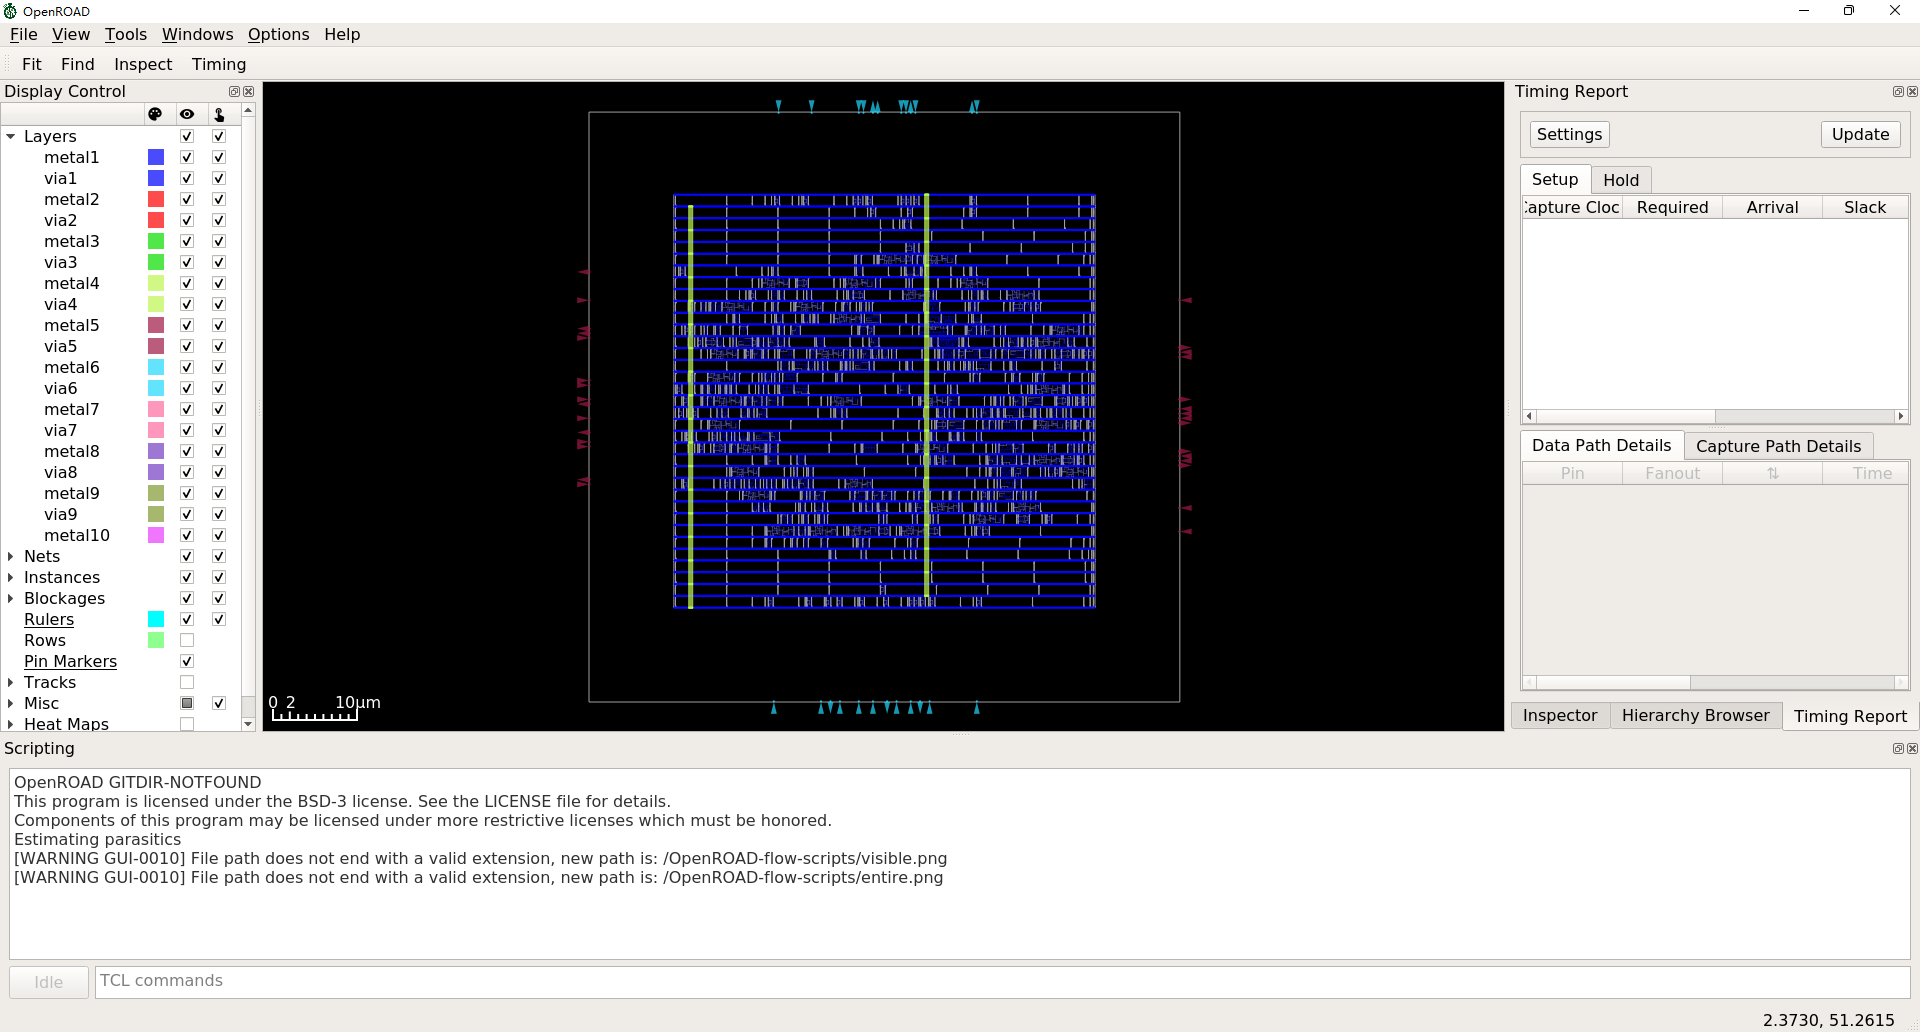
\includegraphics[width=\textwidth]{images/3.png}
\end{figure}
\subsubsection{Global Routing}
Run \texttt{make route} and examine the output:
\begin{enumerate}
    \item Generate routing grid
    \begin{minted}{text}
[INFO GRT-0053] Routing resources analysis:
          Routing      Original      Derated      Resource
Layer     Direction    Resources     Resources    Reduction (%)
---------------------------------------------------------------
metal1     Horizontal          0             0          0.00%
metal2     Vertical        11979          5568          53.52%
metal3     Horizontal      16335          7776          52.40%
metal4     Vertical         7623          5362          29.66%
metal5     Horizontal       7623          5408          29.06%
metal6     Vertical         7623          5408          29.06%
metal7     Horizontal       2178          1120          48.58%
metal8     Vertical         2178          1120          48.58%
metal9     Horizontal       1089          1024          5.97%
metal10    Vertical         1089          1024          5.97%
---------------------------------------------------------------
    \end{minted}
    \item Perform global routing
    \begin{minted}[breaklines,breakanywhere]{text}
[INFO GRT-0096] Final congestion report:
Layer         Resource        Demand        Usage (%)    Max H / Max V / Total Overflow
---------------------------------------------------------------------------------------
metal1               0             0            0.00%             0 /  0 /  0
metal2            5568           743           13.34%             0 /  0 /  0
metal3            7776           773            9.94%             0 /  0 /  0
metal4            5362            79            1.47%             0 /  0 /  0
metal5            5408             4            0.07%             0 /  0 /  0
metal6            5408             0            0.00%             0 /  0 /  0
metal7            1120             0            0.00%             0 /  0 /  0
metal8            1120             0            0.00%             0 /  0 /  0
metal9            1024             0            0.00%             0 /  0 /  0
metal10           1024             0            0.00%             0 /  0 /  0
---------------------------------------------------------------------------------------
Total            33810          1599            4.73%             0 /  0 /  0
    \end{minted}
    \item Check for antenna violations
    \begin{minted}{text}
[INFO ANT-0002] Found 0 net violations.
[INFO ANT-0001] Found 0 pin violations.
    \end{minted}
\end{enumerate}
\subsubsection{Detailed Routing}
\begin{enumerate}
    \item Region query
    \begin{minted}{text}
[INFO DRT-0168] Init region query.
[INFO DRT-0024]   Complete active.
[INFO DRT-0024]   Complete Fr_VIA.
[INFO DRT-0024]   Complete metal1.
[INFO DRT-0024]   Complete via1.
...
    \end{minted}
    \item Pin access
    \begin{minted}{text}
[INFO DRT-0165] Start pin access.
[INFO DRT-0076]   Complete 100 pins.
[INFO DRT-0078]   Complete 176 pins.
[INFO DRT-0081]   Complete 53 unique inst patterns.
[INFO DRT-0084]   Complete 260 groups.
    \end{minted}
    \item Post-process guides
    \begin{minted}{text}
[INFO DRT-0169] Post process guides.
[INFO DRT-0176] GCELLGRID X 0 DO 33 STEP 4200 ;
[INFO DRT-0177] GCELLGRID Y 0 DO 33 STEP 4200 ;
[INFO DRT-0028]   Complete active.
[INFO DRT-0028]   Complete Fr_VIA.
[INFO DRT-0028]   Complete metal1.
[INFO DRT-0028]   Complete via1.
    \end{minted}
    \item Track assignment
    \begin{minted}[breaklines]{text}
[INFO DRT-0181] Start track assignment.
[INFO DRT-0184] Done with 885 vertical wires in 1 frboxes and 1520 horizontal wires in 1 frboxes.
[INFO DRT-0186] Done with 186 vertical wires in 1 frboxes and 316 horizontal wires in 1 frboxes.
[INFO DRT-0182] Complete track assignment.
    \end{minted}
    \item Detailed routing
    \begin{minted}{text}
[INFO DRT-0194] Start detail routing.
[INFO DRT-0195] Start 0th optimization iteration.
    Completing 10% with 0 violations.
    elapsed time = 00:00:00, memory = 113.23 (MB).
    Completing 20% with 0 violations.
    elapsed time = 00:00:00, memory = 112.47 (MB).
    Completing 30% with 0 violations.
...
    Completing 100% with 31 violations.
    elapsed time = 00:00:01, memory = 130.37 (MB).
[INFO DRT-0199]   Number of violations = 160.
Viol/Layer      metal1   via1 metal2 metal3 metal4 metal5
Cut Spacing          0      1      0      0      0      0
Metal Spacing        2      0      8      0      0      0
Recheck              0      0     87     32      9      1
Short                1      0     18      1      0      0
...
[INFO DRT-0199]   Number of violations = 0.
...
[INFO DRT-0198] Complete detail routing.
Total wire length = 3568 um.
    \end{minted}
\end{enumerate}
See this step in the GUI:
\begin{minted}{bash}
make gui_route
\end{minted}
\begin{figure}[H]
    \centering
    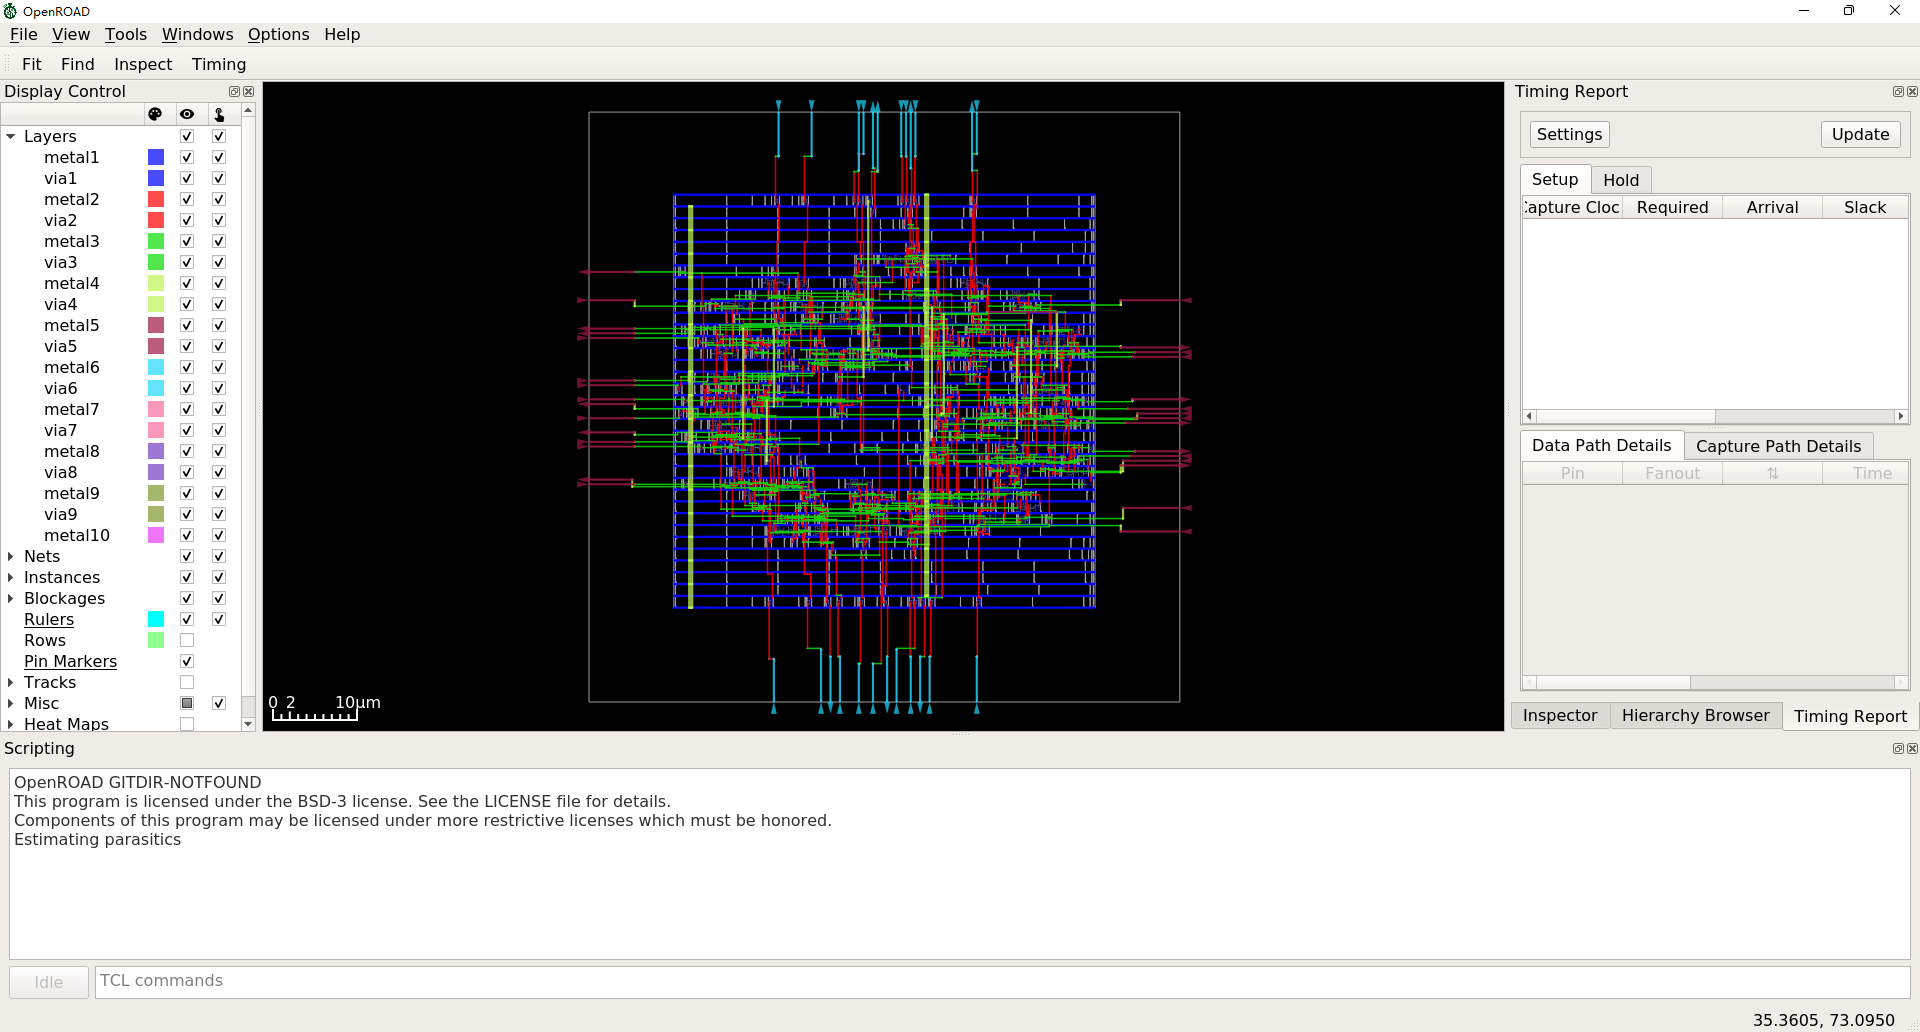
\includegraphics[width=\textwidth]{images/4.png}
\end{figure}
\subsubsection{Parasitic Extraction}
Run \texttt{make finish} and examine the output:

Extract parasitic capacitances and resistances
\begin{minted}[breaklines]{text}
[INFO RCX-0008] extracting parasitics of gcd ...
[INFO RCX-0435] Reading extraction model file ./platforms/nangate45/rcx_patterns.rules ...
[INFO RCX-0436] RC segment generation gcd (max_merge_res 50.0) ...
[INFO RCX-0040] Final 1291 rc segments
[INFO RCX-0439] Coupling Cap extraction gcd ...
...
[INFO RCX-0017] Finished writing SPEF ...
\end{minted}
\subsubsection{Timing Signoff}
\begin{enumerate}
    \item Report final timing
    \begin{minted}[breaklines,breakanywhere]{text}
==========================================================================
finish report_tns
--------------------------------------------------------------------------
tns -1.50

==========================================================================
finish report_wns
--------------------------------------------------------------------------
wns -0.09

==========================================================================
finish report_worst_slack
--------------------------------------------------------------------------
worst slack -0.09

==========================================================================
finish report_clock_skew
--------------------------------------------------------------------------
Clock core_clock
Latency      CRPR       Skew
_699_/CK ^
   0.05
_688_/CK ^
   0.05      0.00       0.00
    \end{minted}
    \item Report final electrical violations
    \begin{minted}[breaklines,breakanywhere]{text}
==========================================================================
finish max_slew_violation_count
--------------------------------------------------------------------------
max slew violation count 0

==========================================================================
finish max_fanout_violation_count
--------------------------------------------------------------------------
max fanout violation count 0

==========================================================================
finish max_cap_violation_count
--------------------------------------------------------------------------
max cap violation count 0

==========================================================================
finish setup_violation_count
--------------------------------------------------------------------------
setup violation count 0

==========================================================================
finish hold_violation_count
--------------------------------------------------------------------------
hold violation count 1
    \end{minted}
\end{enumerate}
See this step in the GUI:
\begin{minted}{bash}
make gui_finish
\end{minted}
\subsubsection{GDS Export}
Export DEF file to GDS file
\begin{minted}[breaklines]{text}
[INFO] Reading DEF ...
[INFO] Clearing cells...
[INFO] Merging GDS/OAS files...
        ./platforms/nangate45/gds/NangateOpenCellLibrary.gds
[INFO] Copying toplevel cell 'gcd'
WARNING: no fill config file specified
[INFO] Checking for missing cell from GDS/OAS...
[INFO] Found GDS_ALLOW_EMPTY variable.
[INFO] All LEF cells have matching GDS/OAS cells
[INFO] Checking for orphan cell in the final layout...
[INFO] No orphan cells
[INFO] Writing out GDS/OAS 'results/nangate45/gcd/base/6_1_merged.gds'
\end{minted}
See this step in the GUI:
\begin{figure}[H]
    \centering
    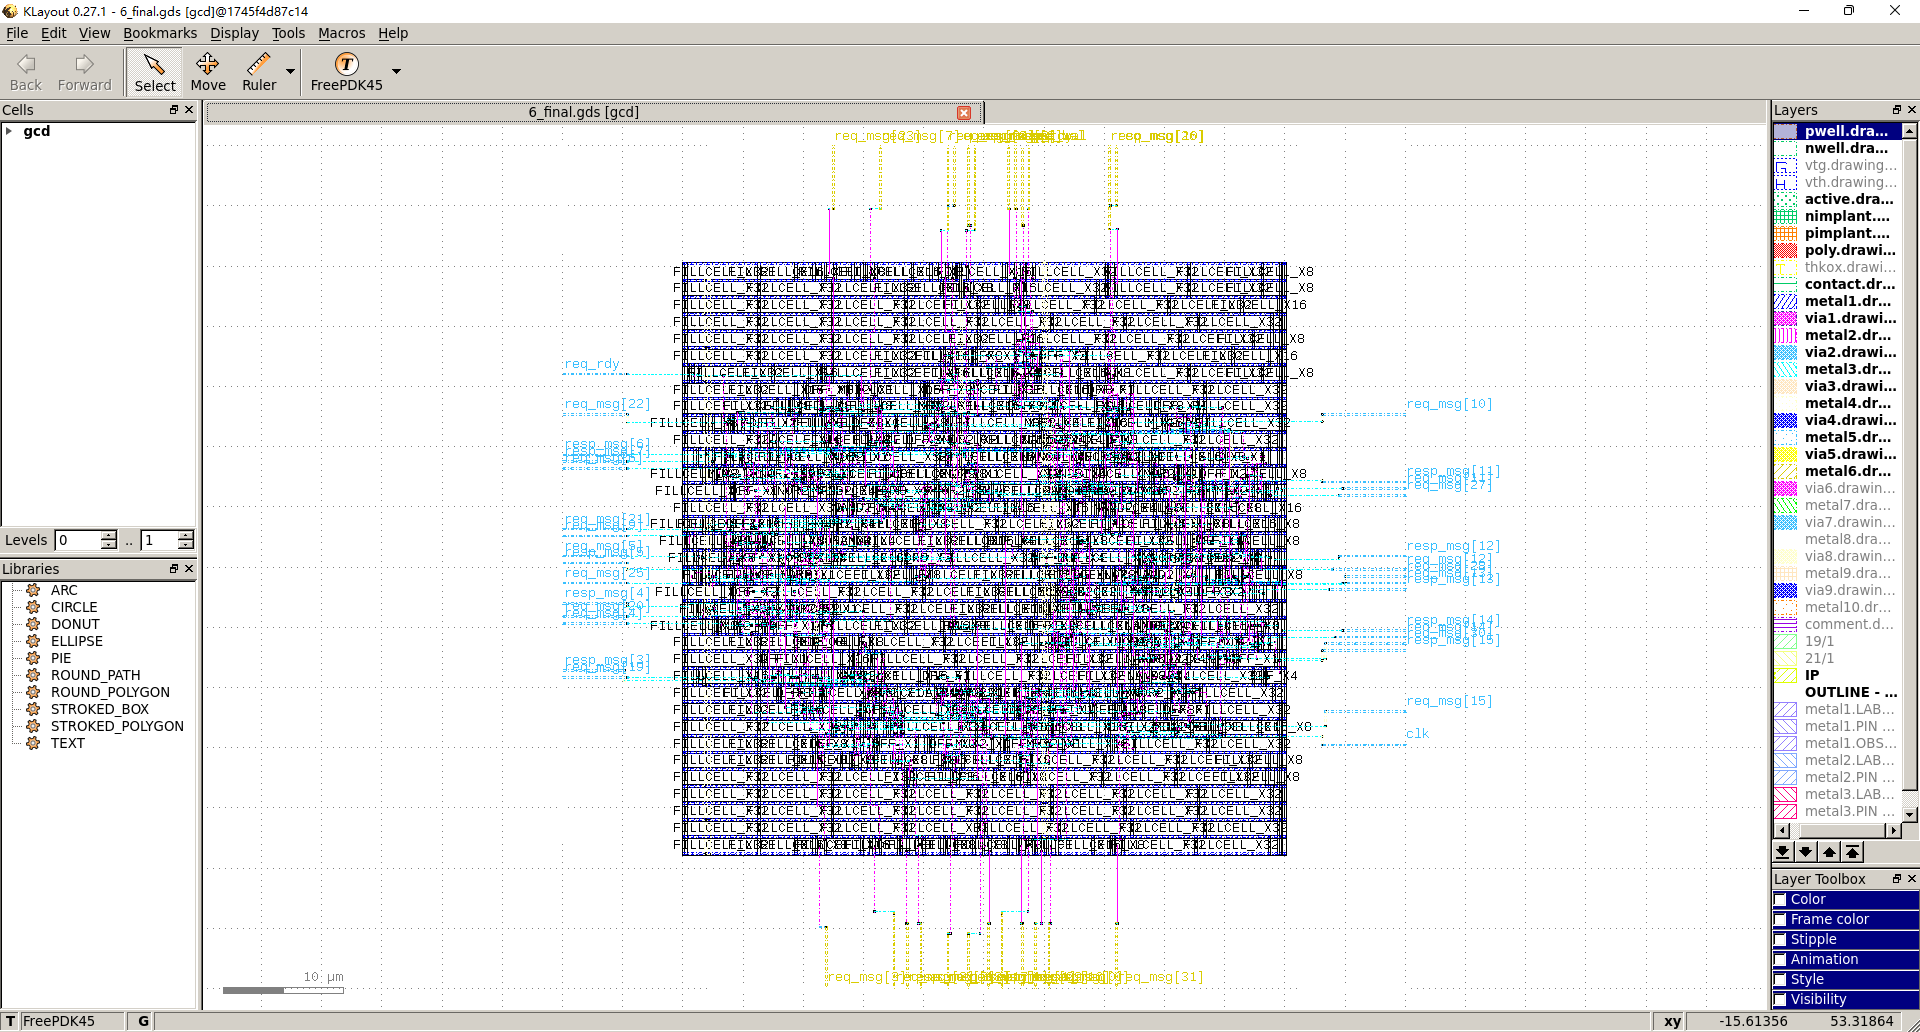
\includegraphics[width=\textwidth]{images/5.png}
\end{figure}
\subsection{Questions}
\begin{enumerate}
    \item What is half perimeter wire length?
    \item What does the Nesterov gradient descent do in global placement?
    \item During global placement, the half perimeter wire length, worst slack, and the number of weighted nets when the iteration number of the second Nesterov gradient descent is 320, and the final RC value.
    \item What do the global placement and the detailed placement do?
    \item What are the names of algorithms that the global placement use? What are the names of algorithms that the detailed placement use?
    \item Select one algorithm you list above and briefly introduce the core part of the algorithm.
    \item What are the post-pair critical path delay and slack during the clock-tree synthesis?
    \item What is the name of the algorithm that the global routing use? What is the name of the algorithm that the detailed routing use?
    \item What is parasitic extraction?
    \item What are the finish critical path delay and slack during the timing signoff?
\end{enumerate}
\subsection{Exercise 1: Debugging a Design \#1}\label{SE1}
Copy files in \texttt{lab6\_starter} to your workspace and bind mount to Docker.

Find the problem with the provided design.

\texttt{../../exercise1/config.mk} provides a faulty design config for the design \texttt{dynamic\_node}, which is a mesh router node. Find the error by running:
\begin{minted}{bash}
make DESIGN_CONFIG=../../exercise1/config.mk
\end{minted}
Once the error is spotted, open \texttt{../../exercise1/config.mk} in a text editor and fix the problematic line(s). You can test your solution by cleaning and rerunning the design:
\begin{minted}{bash}
# Save time by only cleaning the floorplan step to avoid rerunning synthesis
make DESIGN_CONFIG=../../exercise1/config.mk clean_floorplan
make DESIGN_CONFIG=../../exercise1/config.mk
\end{minted}
\subsection{Exercise 2: Debugging a Design \#2}\label{SE2}
Find the problem with the provided design

\texttt{../../exercise2/config.mk} provides a faulty design config. Find the error by running:
\begin{minted}{bash}
make DESIGN_CONFIG=../../exercise2/config.mk
\end{minted}
Once the error is spotted, open \texttt{../../exercise2/config.mk} in a text editor and fix the problematic line(s). You can test your solution by cleaning and rerunning the design:
\begin{minted}{bash}
# Save time by only cleaning the floorplan step to avoid rerunning synthesis
make DESIGN_CONFIG=../../exercise2/config.mk clean_floorplan
make DESIGN_CONFIG=../../exercise2/config.mk
\end{minted}
\subsubsection{Analyzing Your Design Using OpenROAD}
Follow along as the slides demonstrate how to observe design metrics.

This demo will look at the metrics reported for \texttt{nangate45/gcd}. If you haven't already, run the design by running make.

Once complete, observe the final report by navigating to \texttt{logs/nangate45/gcd/base/\\
6\_report.json} for a simple JSON-based report or \texttt{logs/nangate45/gcd/base/6\_report.log} for a textual report.
\subsubsection{Modeling Power}
To observe the modeled power, look at \texttt{finish\_\_power\_\_total} or \texttt{finish report\_power}. Note that OpenROAD models power using default activity factors on inputs and propagates these activity factors through the design. This method provides a solid first-order approximation of power and is useful for design space exploration. You can increase the accuracy of the model by applying accurate activity factors on the inputs (see OpenSTA documentation). Static activity-based power modeling (SAIF) and vector-based (VPD) power modeling are even more accurate methods; however, they are not currently supported in OpenROAD.

OpenROAD power report:
\begin{minted}[breaklines,breakanywhere]{text}
==========================================================================
finish report_power
--------------------------------------------------------------------------
Group                  Internal  Switching    Leakage      Total
                          Power      Power      Power      Power (Watts)
----------------------------------------------------------------
Sequential             4.50e-04   5.96e-05   3.16e-06   5.13e-04  31.9%
Combinational          5.65e-04   5.20e-04   9.95e-06   1.10e-03  68.1%
Macro                  0.00e+00   0.00e+00   0.00e+00   0.00e+00   0.0%
Pad                    0.00e+00   0.00e+00   0.00e+00   0.00e+00   0.0%
----------------------------------------------------------------
Total                  1.02e-03   5.80e-04   1.31e-05   1.61e-03 100.0%
                          63.2%      36.0%       0.8%
\end{minted}
Total power is the most important metric; however, you can read more about the other components \href{https://blogs.cuit.columbia.edu/zp2130/modeling_power_terminology}{here}. The power report is broken down by group, where \texttt{Sequential} represents flip-flops, \texttt{Combinational} represents logic gates, \texttt{Macro} represents macros such as SRAM, and \texttt{Pad} represents I/O cells (if any).
\subsubsection{Calculating Max Frequency}
To determine the maximum frequency, look at \texttt{finish\_\_timing\_\_setup\_\_ws} or finish \texttt{report\_worst\_slack} value. "Slack" is the difference between the constraint (0.46ns) and the actual signal propagation time. Positive slack means the constraint is met ("there is extra slack"). Negative slack means the constraint is violated.
\begin{minted}[breaklines,breakanywhere]{text}
==========================================================================
finish report_worst_slack
--------------------------------------------------------------------------
worst slack -0.09
\end{minted}
Using the slack, the frequency is calculated as:
\begin{equation}
    \mathrm{Frequency_{max}=\frac{1}{constraint-slack}}
\end{equation}
Be mindful of the sign and units of the slack. Greater slack should mean greater frequency. Be sure that you also calculate frequency using \textit{setup} slack, not \textit{hold} slack.

In this case, the max frequency is:
\begin{equation}\label{EEq1}
    \mathrm{Frequency_{max}=\frac{1}{constraint-slack}=}\dots
\end{equation}
    % \mathrm{Frequency_{max}=\frac{1}{constraint-slack}=\frac{1}{0.46ns-(-0.09ns)}\approx1.82GHz}
\subsubsection{Measuring Area}
To measure the design area, you must be aware of the different types of the reported area.
\begin{enumerate}
    \item Synthesized area\\
    The synthesized area is obtained after synthesis and is a good first-order model for design space exploration. You can find the design area in \texttt{reports/nangate45/gcd/\\
    base/synth\_stat.txt}. Units are $\mathrm{\mu m^2}$.
    \begin{minted}[breaklines,breakanywhere]{text}
   Chip area for module '\gcd': 519.764000
    \end{minted}
    \item Place-and-route area\\
    Place-and-route area is the area obtained after cell placement and routing. If reporting this number, it is implied that the design does not have any violations which make the chip unmanufacturable (e.g., routing or hold time violations). You can find the area from \texttt{finish\_\_design\_\_instance\_\_area} or \texttt{finish report\_design\_area}.
    \begin{minted}[breaklines,breakanywhere]{text}
==========================================================================
finish report_design_area
--------------------------------------------------------------------------
Design area 584 u^2 24% utilization.
    \end{minted}
    \item Core area/die area\\
    Core / Die areas are the most accurate numbers, as they specify the exact area of silicon that will be used for fabrication. However, these numbers are not often reported for computer architecture works. The core area is the area of silicon that cells can occupy. It can effectively be calculated as:
    \begin{equation}
        \mathrm{Area_{core}=\frac{Area_{design}}{utilizaiton}}
    \end{equation}
    The Die area includes all silicon areas needed to fabricate the chip, including any I/O and utilized space.\\
    In the case of \texttt{nangate45/gcd}, the easiest location to find this information is from the design config, which specifies the die area as a set of $(x_1,y_1,x_2,y_2)$ coordinates:\\
    flow/designs/nangate45/gcd/config.mk:
    \begin{minted}{Makefile}
export DIE_AREA    = 0 0 70.11 70
export CORE_AREA   = 10.07 11.2 60.04 60.2
    \end{minted}
    yielding a die area of:
    \begin{equation}\label{EEq2}
        \mathrm{Area_{die}=}\dots
    \end{equation}
        % \mathrm{Area_{die}=(70.11\mu m-0\mu m)\times(70\mu m-0\mu m)=4907.7\mu m^2}
    and core area of:
    \begin{equation}\label{EEq3}
        \mathrm{Area_{core}=}\dots
    \end{equation}
        % \mathrm{Area_{core}=(60.04\mu m-10.07\mu m)\times(60.2\mu m-11.2\mu m)=2448.53\mu m^2}
    which can also be obtained from the previous formula:
    \begin{equation}\label{EEq4}
        \mathrm{Area_{core}=\frac{Area_{design}}{utilizaiton}=}\dots
    \end{equation}
        % \mathrm{Area_{core}=\frac{Area_{design}}{utilizaiton}=\frac{584\mu m^2}{0.24}=2433.33\mu m^2}
\end{enumerate}
\subsection{Exercise 3: Creating a Pareto Curve}\label{SE3}
Adjust the constraints on a design to observe the impact on power, performance, and area (PPA).

\texttt{../../exercise3/} provides a simple integer arithmetic logic unit (ALU). The default bitwidth is 12, and the default clock constraint is 7ns ($\sim$143 MHz). These parameters allow for RTL-to-GDS in under 1 minute. Run the design with:
\begin{minted}{bash}
make DESIGN_CONFIG=../../exercise3/config.mk
\end{minted}
Once complete, observe the final report at \texttt{logs/nangate45/alu/base/6\_report.json} or \texttt{logs/nangate45/alu/base/6\_report.log}.

Record the power, frequency, and area. Then, open the constraint file (\texttt{../../exercise3/\\
constraint.sdc}) with your favorite editor and adjust the clock period to 6ns.

Clean the design and rerun using the new constraint:
\begin{minted}{bash}
make DESIGN_CONFIG=../../exercise3/config.mk clean_all
make DESIGN_CONFIG=../../exercise3/config.mk
\end{minted}

Once complete, you can plot this data using your favorite software (Google Sheets, Microsoft Excel, \texttt{matplotlib}, etc.). Use max frequency as the independent variable.
\subsection{Exercise 4: Scaling a Design Across Technologies}\label{SE4}
Observe the differences when a design is implemented in different technologies.

OpenROAD-flow-scripts provides three open-source PDKs to implement designs in SkyWater 130nm, Nangate 45nm, and ASAP 7nm. RTL is easily portable across technologies if it does not contain technology-specific cells (such as I/O pads, SRAM, clock-gate cells, etc.).

The \texttt{../../exercise4/} directory contains the same ALU design from Exercise 3. However, this time you will change the config to alter the target technology. Adjust the \texttt{PLATFORM} variable in \texttt{../../exercise4/config.mk} to to one of the technologies (\texttt{sky130hd}, \texttt{nangate45}, \texttt{asap7}). Keep in mind that:
\begin{itemize}
    \item You may need to clean the design data from Exercise 3, because the platform and design name (\texttt{nangate45/alu}) are reused:
    \begin{minted}{bash}
make DESIGN_CONFIG=../../exercise3/config.mk clean_all
    \end{minted}
    \item The time units for \texttt{sky130hd} and \texttt{nangate45} are both in ns, but the units for \texttt{asap7} are in ps. In order to maintain parity, you will need to adjust \texttt{../../exercise4/\\
    constraint.sdc}.
\end{itemize}
Then, run the design using:
\begin{minted}{bash}
make DESIGN_CONFIG=../../exercise4/config.mk
\end{minted}
Record the power, frequency, and area for each technology. You need not clean the design between runs because changing the platform changes the output directory. You can again graph the data using your favorite graphing software.
\subsection{Building Complex Designs}\label{SComplex}
Follow along as the slides explain how to incorporate macros into your design.

For designs to scale to larger sizes, additional layers of abstraction are required. Macros are special cells that are not logic gates and aren't automatically generated from synthesis. Macros are often much larger than standard cells and therefore require special handling. Macros are often used for several reasons:
\begin{enumerate}
    \item Using SRAM or register files for large memories
    \item Encapsulating a module that is instantiated multiple times
    \item I/O pad cells for off-chip power and communication
    \item Fiducial cells required by the manufacturer for fabrication
    \item Intellectual property (IP) provided by a third-party vendor
    \item And more!
\end{enumerate}
\subsubsection{How can I generate macros?}
\begin{itemize}
    \item \href{https://github.com/VLSIDA/OpenRAM}{OpenRAM} is an open-source SRAM generator
    \begin{itemize}
        \item Requires bitcells and sense amplifiers; creates implementations suitable for fabrication
    \end{itemize}
    \item \href{https://github.com/bespoke-silicon-group/bsg_fakeram}{bsg\_fakeram} is a blackbox SRAM generator
    \begin{itemize}
        \item Creates a blackbox implementation which is useful for modeling; cannot be used for fabrication
    \end{itemize}
    \item Generate a block using OpenROAD
    \begin{itemize}
        \item Use OpenROAD to create a hardened macro, then instantiate the block in a parent module
    \end{itemize}
    \item Acquire third-party IP
    \begin{itemize}
        \item Many commercial vendors provide RAM generators, I/O pad cells, analog macros, and more
    \end{itemize}
\end{itemize}
\texttt{nangate45/tinyRocket} is a CPU core which incorporates SRAM macros generated by \texttt{bsg\_fakeram}. While OpenROAD-flow-scripts already includes platform files necessary for standard cells, designers must specify macro files in the design config.

\texttt{flow/designs/nangate45/tinyRocket/config.mk}:
\begin{minted}[breaklines]{Makefile}
export ADDITIONAL_LEFS = $(sort $(wildcard ./designs/$(PLATFORM)/$(DESIGN_NICKNAME)/*.lef))
export ADDITIONAL_LIBS = $(sort $(wildcard ./designs/$(PLATFORM)/$(DESIGN_NICKNAME)/*.lib))
\end{minted}
The config file uses the variable \texttt{ADDITIONAL\_LEFS} and \texttt{ADDITIONAL\_LIBS} to reference the abstract physical views (\texttt{.lef}) and timing models (\texttt{.lib}) for the macros. The wildcard commands above are shorthand for:
\begin{minted}[breaklines,breakanywhere]{Makefile}
export ADDITIONAL_LEFS = ./designs/nangate45/tinyRocket/fakeram45_1024x32.lef ./designs/nangate45/tinyRocket/fakeram45_64x32.lef
export ADDITIONAL_LIBS = ./designs/nangate45/tinyRocket/fakeram45_1024x32.lib ./designs/nangate45/tinyRocket/fakeram45_64x32.lib
\end{minted}
Notice, however, that these RAMs are generated by \texttt{bsg\_fakeram} and do not have physical implementation files (\texttt{.gds}). Normally, this would create an error during the GDS merge step, however the platform configuration for nangate45 downgrades this to a warning by setting \texttt{GDS\_ALLOW\_EMPTY} on these instances:
\begin{minted}[breaklines,breakanywhere]{Makefile}
# Allow empty GDS cell
export GDS_ALLOW_EMPTY = fakeram.*
\end{minted}
If the macro does have a physical implementation (\texttt{.gds}), it can be added to the design config with:
\begin{minted}[breaklines]{Makefile}
export ADDITIONAL_GDS = /path/to/macro1.gds /path/to/macro2.gds ...
\end{minted}
Now, build tinyRocket with:
\begin{minted}[breaklines]{Makefile}
# Build takes several minutes
make DESIGN_CONFIG=./designs/nangate45/tinyRocket/config.mk
\end{minted}
Once done, you can see that new steps in the flow were used:
\begin{enumerate}
    \item \texttt{2\_3\_tdms\_place.log}: timing-driven mixed-size place
    \item \texttt{2\_4\_mplace.log}: macro place
\end{enumerate}
\texttt{tdms\_place} performs a rough initial placement of both macros and standard cells. This is used as a seed for the macro placer. \texttt{mplace} performs macro placement. The placer tries to ensure that macros block as little design area as possible while still allowing connectivity to the macro.

Common problems when introducing macros:
\begin{itemize}
    \item "Channels" between macros need to be wide enough to not overcongest the router
    \item Slight changes to the design area can cause large changes in the macro placements
    \item Macros can block regions of the core area and make standard cell placement difficult
    \item Malformed macros can cause difficult-to-diagnose design problems
\end{itemize}
\subsection{(Optional) Exercise 5: Setting Up a New Design with OpenROAD-flow-Scripts}\label{SE5}
% If you have your own RTL, now's the time to use it!
Use the provided \texttt{counter.v} file.

The directory \texttt{../../exercise5/} contains a blank config.mk template and blank constraint.sdc template.

% If you have Verilog RTL file(s), place it (them) in ../../exercise5/.
% If you don't have your own RTL, you can use the provided counter.v file instead.
% Feel free to use other designs as a reference! Use any platform you want.
\subsection{Using OpenLane for the Free Skywater 130nm Open MPW Shuttle}
Follow along as the slides explain \href{https://github.com/The-OpenROAD-Project/OpenLane}{OpenLane}, the \href{https://efabless.com/open_shuttle_program}{Efabless OpenMPW Program}, and a \href{https://platform.efabless.com/projects/1165}{design which was just submitted}.

\newpage
\section{Synopsys ASIC Tools}\label{STools}
\subsection{Nangate 45nm Standard-Cell Library}
Before you can gain access to a standard-cell library, you need to gain access to a “physical design kit” (PDK). A PDK includes all of the design files required for full-custom circuit design for a specific technology. So this will include a design-rule manual as well as SPICE circuit models for transistors and other devices. Gaining access to a real PDK is difficult. It requires negotiating with the foundry and signing multiple non-disclosure agreements. So in this lab we will be using the FreePDK45 PDK:

\url{https://eda.ncsu.edu/freepdk/freepdk45/}

This is an open PDK for a “fake” technology. It was created by universities using publically available data on several different commercial 45nm processes. This means you cannot actually tapeout a chip using this PDK, but the technology is representative enough to provide reasonable area, energy, and timing estimates for research and teaching purposes. You can find the FreePDK45 PDK installed here:
\begin{minted}{bash}
cd /home/users/ece481/freepdk-45nm/
\end{minted}
A standard-cell designer will use the PDK to implement the standard-cell library. A standard-cell library is a collection of combinational and sequential logic gates that adhere to a standardized set of logical, electrical, and physical policies. For example, all standard cells are usually the same height, include pins that align to a predetermined vertical and horizontal grid, include power/ground rails and nwells in predetermined locations, and support a predetermined number of drive strengths. A standard-cell designer will usually create a high-level behavioral specification (in Verilog), circuit schematics (in SPICE), and the actual layout (in \texttt{.gds} format) for each logic gate. The Synopsys and Cadence tools do not actually use these low-level implementations since they are actually too detailed. Instead, these tools use abstract views of the standard cells, which capture logical functionality, timing, geometry, and power usage at a much higher level.

Just like with a PDK, gaining access to a real standard-cell library is difficult. It requires gaining access to the PDK first, negotiating with a company that makes standard cells, and usually signing more non-disclosure agreements. In this lab, we will be using the Nangate 45nm standard-cell library, which is based on the open FreePDK45 PDK.

Nangate is a company that makes a tool to automatically generate standard-cell libraries, so they have made this library publically available as a way to demonstrate their tool. Since it is an open library, it is a great resource for research and teaching. Even though the standard-cell library is based on a “fake” 45nm PDK, the library provides a very reasonable estimate of a real commercial standard library in a real 45nm technology. In this section, we will take a look at both the low-level implementations and high-level views of the Nangate standard-cell library.

A standard-cell library distribution can contain gigabytes of data in thousands of files. For example, here is the distribution for the Nangate standard-cell library.
\begin{minted}{bash}
cd /home/users/ece481/freepdk-45nm/stdcells.mwlib
\end{minted}
Set the variable \texttt{ECE4810J\_STDCELLS} to the \texttt{freepdk-45nm} directory. ADK means ASIC design kit.
\begin{minted}[breaklines]{text}
% cd $ECE4810J_STDCELLS
% ls
rtk-stream-out.map     # gds layer map
rtk-tech.lef           # interconnect technology information
rtk-tech.tf            # interconnect technology information
rtk-typical.captable   # interconnect technology information
stdcells.gds           # layout for each cell
stdcells.v             # behavioral specification for each cell
stdcells-lpe.spi       # circuit schematics with parasitics for each cell
stdcells.lib           # abstract logical, timing, power view for each cell (typical)
stdcells-bc.lib        # best case .lib
stdcells-wc.lib        # worst case .lib
stdcells.lef           # abstract physical view for each cell
stdcells.db            # binary compiled version of .lib file
stdcells.mwlib         # Milkyway database built from .lef file
stdcells-databook.pdf  # standard-cell library databook
klayout.lyp            # layer settings for Klayout
\end{minted}
Let’s begin by looking at the schematic for a 3-input NAND cell (NAND3\_X1).
\begin{minted}[breaklines]{text}
.SUBCKT NAND3_X1 A1 A2 A3 ZN VDD VSS
*.PININFO A1:I A2:I A3:I ZN:O VDD:P VSS:G
*.EQN ZN=!((A1 * A2) * A3)
M_i_2 net_1 A3 VSS   VSS NMOS_VTL W=0.415000U L=0.050000U
M_i_1 net_0 A2 net_1 VSS NMOS_VTL W=0.415000U L=0.050000U
M_i_0 ZN    A1 net_0 VSS NMOS_VTL W=0.415000U L=0.050000U
M_i_5 ZN    A3 VDD   VDD PMOS_VTL W=0.630000U L=0.050000U
M_i_4 VDD   A2 ZN    VDD PMOS_VTL W=0.630000U L=0.050000U
M_i_3 ZN    A1 VDD   VDD PMOS_VTL W=0.630000U L=0.050000U
.ENDS
\end{minted}
For students with a circuits background, there should be no surprises here, and for those students with fewer circuits backgrounds, we will cover basic static CMOS gate design later in the lab. Essentially, this schematic includes three NMOS transistors arranged in series in the pull-down network and three PMOS transistors arranged in parallel in the pull-up network. The PMOS transistors are larger than the NMOS transistors (see \texttt{W=} parameter) because the mobility of holes is less than the mobility of electrons.

Now let’s look at the layout for the 3-input NAND cell using the open-source Klayout GDS viewer.
\begin{minted}{bash}
klayout -l $ECE4810J_STDCELLS/klayout.lyp $ECE4810J_STDCELLS/stdcells.gds
\end{minted}
Note that we are using the \texttt{.lyp} file, which is a predefined layer color scheme that makes it easier to view GDS files. To view the 3-input NAND cell, find the NAND3\_X1 cell in the left-hand cell list, and then choose \_Display > Show as New Top from the menu. Here is a picture of the layout for this cell.
\begin{figure}[H]
    \centering
    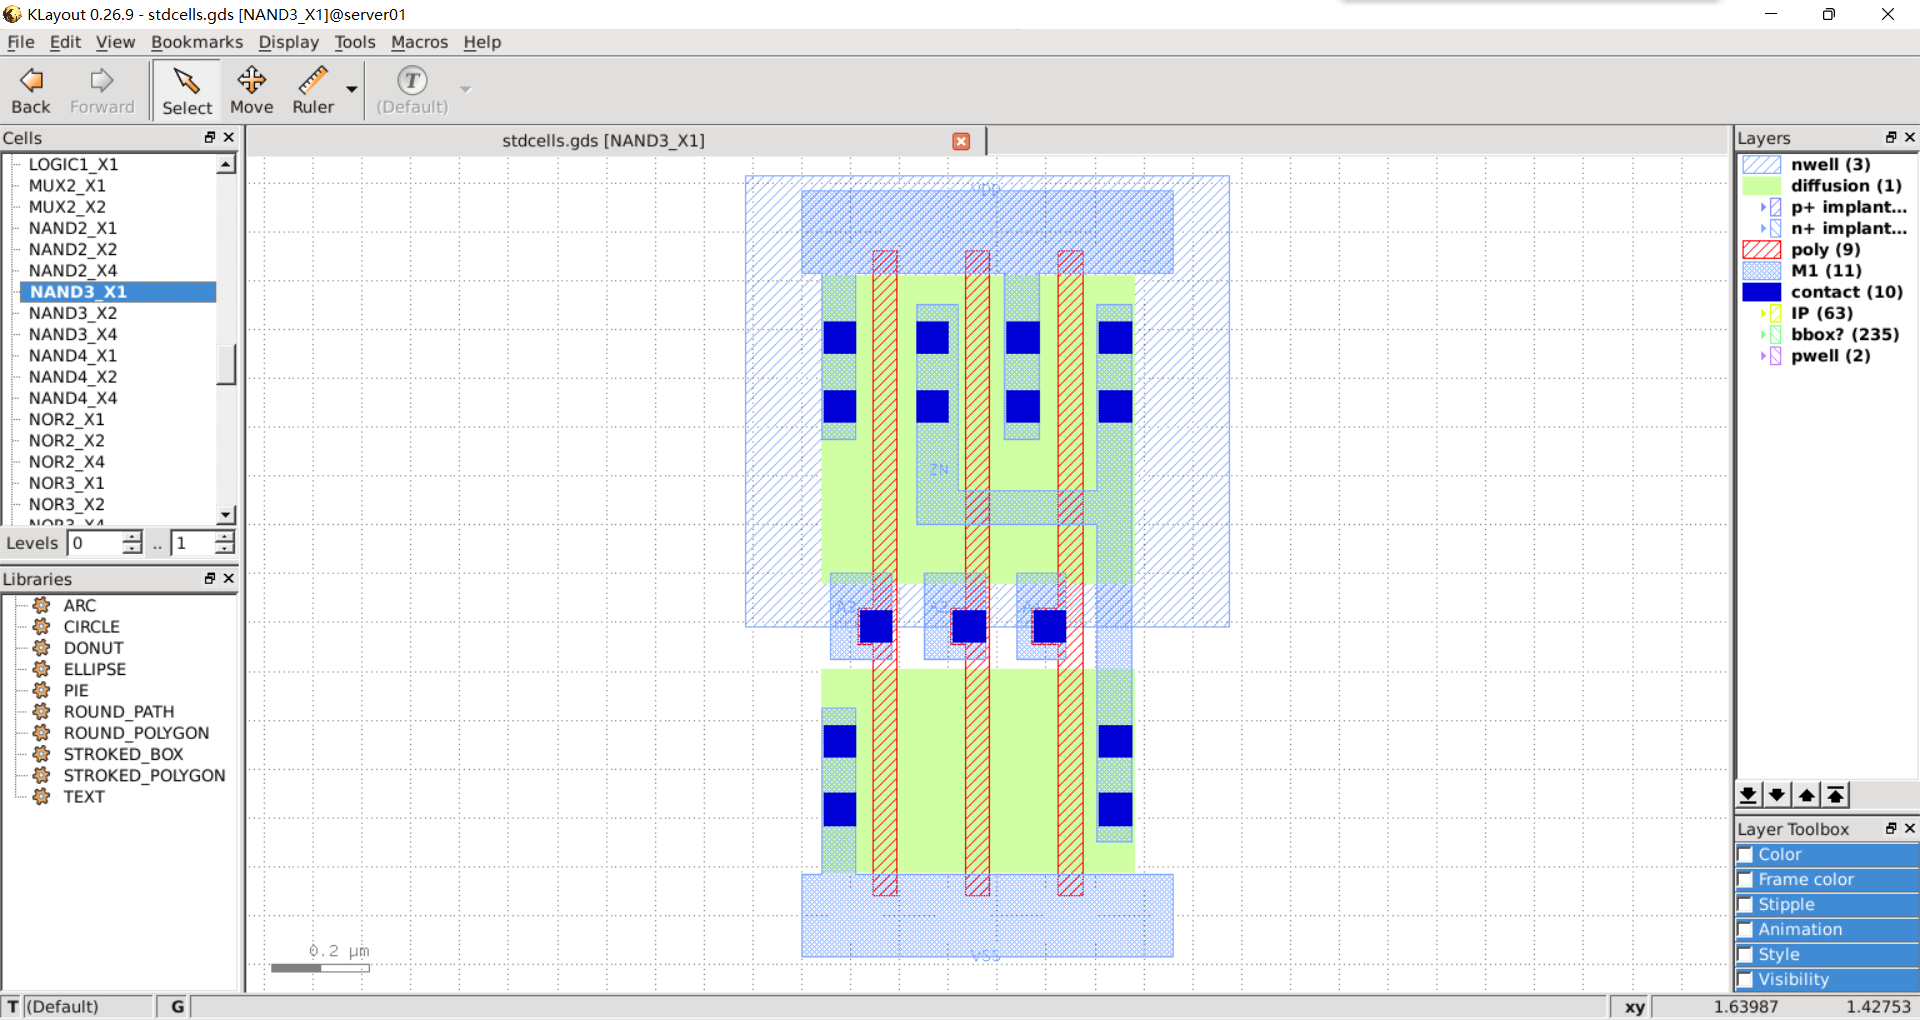
\includegraphics[width=\textwidth]{images/6.png}
\end{figure}
Diffusion is green, polysilicon is red, contacts are solid dark blue, metal 1 (M1) is blue, and the nwell is the large gray rectangle over the top half of the cell. All standard cells will be the same height and have the nwell in the same place. Notice the three NMOS transistors arranged in series in the pull-down network and three PMOS transistors arranged in parallel in the pull-up network. The power rail is the horizontal strip of M1 at the top, and the ground rail is the horizontal strip of M1 at the bottom. All standard cells will have the power and ground rails in the same place, so they will connect via abutment if these cells are arranged in a row. Although it is difficult to see, the three input pins and one output pin are labeled squares of M1, and these pins are arranged to be on a predetermined grid.

Now let’s look at the Verilog behavioral specification for the 3-input NAND cell.
\begin{minted}[breaklines]{text}
% less -p NAND3_X1 $ECE4810J_STDCELLS/stdcells.v
module NAND3_X1 (A1, A2, A3, ZN);
  input A1;
  input A2;
  input A3;
  output ZN;

  not(ZN, i_8);
  and(i_8, i_9, A3);
  and(i_9, A1, A2);

  specify
    (A1 => ZN) = (0.1, 0.1);
    (A2 => ZN) = (0.1, 0.1);
    (A3 => ZN) = (0.1, 0.1);
  endspecify

endmodule
\end{minted}
Note that the Verilog implementation of the 3-input NAND cell looks nothing like the Verilog we used in ECE4810J. This cell is implemented using Verilog primitive gates (e.g., not, and), and it includes a specify block that is used for advanced gate-level simulation with back-annotated delays.

We can use sophisticated tools to extract detailed parasitic resistance and capacitance values from the layout, and then we can add these parasitics to the circuit schematic to create a much more accurate model for experimenting with the circuit timing and power. Let’s look at a snippet of the extracted circuit for the 3-input NAND cell:
\begin{minted}[breaklines]{text}
% less -p NAND3_X1 $ECE4810J_STDCELLS/stdcells-lpe.spi
.SUBCKT NAND3_X1 VDD VSS A3 ZN A2 A1
*.PININFO VDD:P VSS:G A3:I ZN:O A2:I A1:I
*.EQN ZN=!((A1 * A2) * A3)
M_M3 N_ZN_M0_d  N_A3_M0_g N_VDD_M0_s VDD PMOS_VTL W=0.630000U L=0.050000U
M_M4 N_VDD_M1_d N_A2_M1_g N_ZN_M0_d  VDD PMOS_VTL W=0.630000U L=0.050000U
M_M5 N_ZN_M2_d  N_A1_M2_g N_VDD_M1_d VDD PMOS_VTL W=0.630000U L=0.050000U
M_M0 net_1      N_A3_M3_g N_VSS_M3_s VSS NMOS_VTL W=0.415000U L=0.050000U
M_M1 net_0      N_A2_M4_g net_1      VSS NMOS_VTL W=0.415000U L=0.050000U
M_M2 N_ZN_M5_d  N_A1_M5_g net_0      VSS NMOS_VTL W=0.415000U L=0.050000U
C_x_PM_NAND3_X1%VDD_c0 x_PM_NAND3_X1%VDD_39 VSS 3.704e-17
C_x_PM_NAND3_X1%VDD_c1 x_PM_NAND3_X1%VDD_36 VSS 2.74884e-18
C_x_PM_NAND3_X1%VDD_c2 x_PM_NAND3_X1%VDD_26 VSS 2.61603e-16
C_x_PM_NAND3_X1%VDD_c3 N_VDD_M1_d           VSS 6.57971e-17
C_x_PM_NAND3_X1%VDD_c4 x_PM_NAND3_X1%VDD_19 VSS 1.89932e-17
C_x_PM_NAND3_X1%VDD_c5 x_PM_NAND3_X1%VDD_18 VSS 3.74888e-17
C_x_PM_NAND3_X1%VDD_c6 N_VDD_M0_s           VSS 3.64134e-17
...
.ENDS
\end{minted}
The full model is a couple of hundred lines long, so you can see how detailed this model is! The ASIC tools do not really need this much detail. We can use a special set of tools to create a much higher level abstract view of the timing and power of this circuit suitable for use by the ASIC tools. Essentially, these tools run many, many circuit-level simulations to create characterization data stored in a \texttt{.lib} (Liberty) file. Let’s look at the snippet of the \texttt{.lib} file for the 3-input NAND cell.
\begin{minted}[breaklines,breakanywhere]{text}
% less -p NAND3_X1 $ECE4810J_STDCELLS/stdcells.lib
cell (NAND3_X1) {
 drive_strength          : 1;
 area                    : 1.064000;
 cell_leakage_power      : 18.104768;
 leakage_power () {
   when                  : "!A1 & !A2 & !A3";
   value                 : 3.318854;
 }
 ...
 pin (A1) {
   direction             : input;
   related_power_pin     : "VDD";
   related_ground_pin    : "VSS";
   capacitance           : 1.590286;
   fall_capacitance      : 1.562033;
   rise_capacitance      : 1.590286;
 }
 ...
 pin (ZN) {
   direction             : output;
   related_power_pin     : "VDD";
   related_ground_pin    : "VSS";
   max_capacitance       : 58.364900;
   function              : "!((A1 & A2) & A3)";

   timing () {

     related_pin         : "A1";
     timing_sense        : negative_unate;

     cell_fall(Timing_7_7) {
       index_1 ("0.00117378,0.00472397,0.0171859,0.0409838,0.0780596,0.130081,0.198535");
       index_2 ("0.365616,1.823900,3.647810,7.295610,14.591200,29.182500,58.364900");
       values ("0.0106270,0.0150189,0.0204521,0.0312612,0.0528211,0.0959019,0.182032", \
               "0.0116171,0.0160692,0.0215549,0.0324213,0.0540285,0.0971429,0.183289", \
               "0.0157475,0.0207077,0.0261030,0.0369216,0.0585239,0.101654,0.187820", \
               "0.0193780,0.0263217,0.0337702,0.0462819,0.0677259,0.110616,0.196655", \
               "0.0218025,0.0305247,0.0399593,0.0560603,0.0822203,0.125293,0.210827", \
               "0.0229784,0.0334449,0.0447189,0.0640615,0.0959700,0.146382,0.231434", \
               "0.0227986,0.0349768,0.0480836,0.0705081,0.107693,0.167283,0.259623");
     }
     ...

     internal_power () {
       related_pin       : "A1";
       fall_power(Power_7_7) {
         index_1 ("0.00117378,0.00472397,0.0171859,0.0409838,0.0780596,0.130081,0.198535");
         index_2 ("0.365616,1.823900,3.647810,7.295610,14.591200,29.182500,58.364900");
         values ("0.523620,0.538965,0.551079,0.556548,0.561151,0.564018,0.564418", \
                 "0.459570,0.484698,0.509668,0.529672,0.543887,0.554682,0.559331", \
                 "0.434385,0.457202,0.470452,0.498312,0.517651,0.538469,0.550091", \
                 "0.728991,0.630651,0.581024,0.559124,0.551408,0.553714,0.557387", \
                 "1.306597,1.153240,1.010684,0.831268,0.727155,0.657699,0.616287", \
                 "2.170611,1.965158,1.760932,1.459438,1.140559,0.930355,0.781393", \
                 "3.276307,3.084566,2.831754,2.426623,1.913607,1.439055,1.113950");
       }
       ...
     }
 ...
}
\end{minted}
This is just a small subset of the information included in the \texttt{.lib} file for this cell. We will talk more about the details of such \texttt{.lib} files later in the lab, but you can see that the \texttt{.lib} file contains information about the area, leakage power, the capacitance of each input pin, logical functionality, and timing. Units for all data are provided at the top of the \texttt{.lib} file. In this snippet, you can see that the area of the cell is 1.064 square microns, and the leakage power is 18.1nW. The capacitance for the input pin \texttt{A1} is 1.59fF, although there is additional data that captures how the capacitance changes depending on whether the input is rising or falling. The output pin \texttt{ZN} implements the logic equation \verb|!((A1 & A2) & A3)| (i.e., a three-input NAND gate). Data within the \texttt{.lib} file is often represented using one- or two-dimensional lookup tables (i.e., a \texttt{values} table). You can see two such tables in the above snippet.

Let’s start by focusing on the first table. This table captures the delay from input pin \texttt{A1} to output pin \texttt{ZN} as a function of two parameters: the input transition time (horizontal direction in a lookup table) and the load capacitance (vertical direction in a lookup table). Note that this delay is when \texttt{ZN} is “falling” (i.e., when it is transitioning from high to low). There is another table for the delay when \texttt{ZN} is rising, and there are additional tables for every input. Gates are slower when the inputs take longer to transition and/or when they are driving large output loads. Each entry in the lookup table reflects the characterization of one or more detailed circuit-level simulations. So in this example, the delay from input pin \texttt{A1} to output pin \texttt{ZN} is 16ps when the input transition rate is 4.7ps, and the output load is 1.82fF. This level of detail can enable very accurate static timing analysis of our designs.

Let’s now focus on the second table. This table captures the internal power, which is the power consumed within the gate itself, again as a function of two parameters: the input transition time (horizontal direction in the lookup table) and the load capacitance (vertical direction in the lookup table). Each entry in the lookup table is calculated by measuring the current drawn from the power supply during a detailed SPICE simulation and \textit{subtracting} any current used to charge the output load. In other words, all of the energy that is \textit{not} consumed charging up the output load is considered internal energy. Note that sometimes the internal power is negative. This is simply due to how we account for energy. We can either assume all energy is consumed only when the output node is charged, and no energy is consumed when the output node is discharged, or we can assume half the energy is consumed when the output node is charged, and half the energy is consumed when the output node is discharged in which case you will sometimes see negative internal power.

Note that some of the ASIC tools actually do not use the \texttt{.lib} file directly, but instead, use a pre-compiled binary version of the \texttt{.lib} file stored in \texttt{.db} format. The binary \texttt{.db} file is usually much more compact that the text \texttt{.lib} file. The \texttt{.lib} file captures the abstract logical, timing, and power aspects of the standard-cell library, but it does not capture the physical aspects of the standard-cell library. While the ASIC tools could potentially use the \texttt{.gds} file directly, the ASIC tools do not really need this much detail. We can use a special set of tools to create a much higher-level abstract view of the physical aspects of the cell suitable for use by the ASIC tools. These tools create \texttt{.lef} files. Let’s look at the snippet of the \texttt{.lef} file for the 3-input NAND cell.
\begin{minted}[breaklines,breakanywhere]{text}
 % less -p NAND3_X1 $ECE4810J_STDCELLS/stdcells.lef
MACRO NAND3_X1
  CLASS core ;
  FOREIGN NAND3_X1 0.0 0.0 ;
  ORIGIN 0 0 ;
  SYMMETRY X Y ;
  SITE FreePDK45_38x28_10R_NP_162NW_34O ;
  SIZE 0.76 BY 1.4 ;

  PIN A1
    DIRECTION INPUT ;
    ANTENNAPARTIALMETALAREA 0.0175 LAYER metal1 ;
    ANTENNAPARTIALMETALSIDEAREA 0.0715 LAYER metal1 ;
    ANTENNAGATEAREA 0.05225 ;
    PORT
      LAYER metal1 ;
        POLYGON 0.44 0.525 0.54 0.525 0.54 0.7 0.44 0.7  ;
    END
  END A1

  PIN ZN
    DIRECTION OUTPUT ;
    ANTENNAPARTIALMETALAREA 0.1352 LAYER metal1 ;
    ANTENNAPARTIALMETALSIDEAREA 0.4992 LAYER metal1 ;
    ANTENNADIFFAREA 0.197925 ;
    PORT
      LAYER metal1 ;
        POLYGON 0.235 0.8 0.605 0.8 0.605 0.15 0.675 0.15
         0.675 1.25 0.605 1.25 0.605 0.87 0.32 0.87 0.32 1.25 0.235 1.25  ;
    END
  END ZN

  PIN VDD
    DIRECTION INOUT ;
    USE power ;
    SHAPE ABUTMENT ;
    PORT
      LAYER metal1 ;
        POLYGON 0 1.315 0.04 1.315 0.04 0.975 0.11 0.975 0.11 1.315
         0.415 1.315 0.415 0.975 0.485 0.975 0.485 1.315 0.76 1.315 0.76 1.485 0 1.485  ;
    END
  END VDD

  ...
END NAND3_X1
\end{minted}
This is just a small subset of the information included in the \texttt{.lef} file for this cell. You can see the \texttt{.lef} file includes information on the dimensions of the cell and the location and dimensions of both power/ground and signal pins. The file also includes information on “obstructions” (or blockages) indicated with a \texttt{OBS} entry. Take a look at the NAND4\_X4 gate to see an obstruction. These are regions of the cell that should not be used by the ASIC tools. For example, if a cell needs to use metal 2 (M2), it would create a blockage on M2 so that the ASIC tools know not to route any M2 wires in that area. You can use Klayout to view \texttt{.lef} files as well.
\begin{minted}{bash}
klayout
\end{minted}
Choose \textit{File > Import > LEF} from the menu. Navigate to the \texttt{stdcells.lef} file. Here is a picture of the \texttt{.lef} for this cell.
\begin{figure}[H]
    \centering
    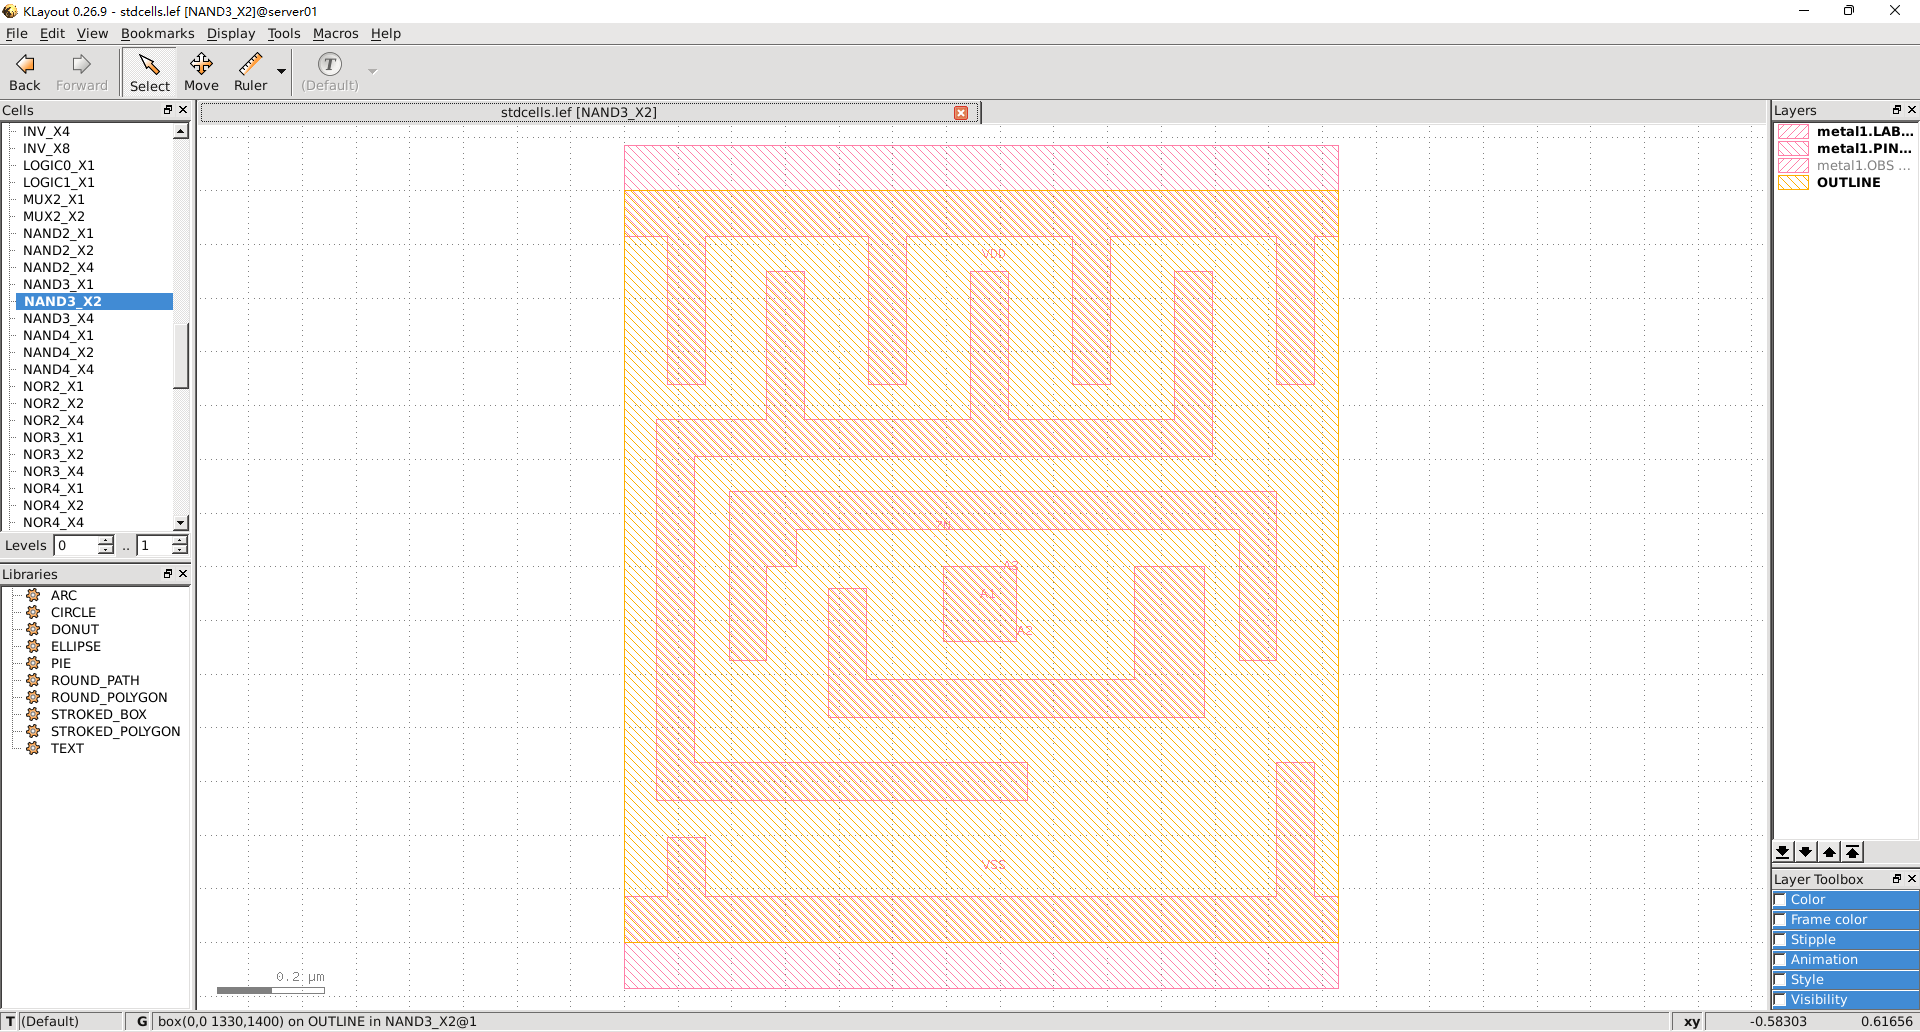
\includegraphics[width=\textwidth]{images/7.png}
\end{figure}
If you compare the \texttt{.lef} to the \texttt{.gds} you can see that the \texttt{.lef} is a much simpler representation that only captures the boundary, pins, and obstructions.

The standard-cell library also includes several files (e.g., \texttt{rtk-tech.tf}, \texttt{rtk-tech.lef}, \texttt{rtk-typical.captable}) that capture information about the metal interconnect including the wire width, pitch, and parasitics. For example, let’s take a look at the \texttt{.captable} file:
\begin{minted}[breaklines,breakanywhere]{text}
% less -p M1 $ECE4810J_STDCELLS/rtk-typical.captable
LAYER M1
   MinWidth              0.07000
   MinSpace              0.06500
#  Height                0.37000
   Thickness             0.13000
   TopWidth              0.07000
   BottomWidth           0.07000
   WidthDev              0.00000
   Resistance            0.38000

END
...
M1
width(um)  space(um) Ctot(Ff/um)  Cc(Ff/um)    Carea(Ff/um) Cfrg(Ff/um)
0.070       0.052       0.1986       0.0723       0.0311       0.0115
0.070       0.065       0.1705       0.0509       0.0311       0.0143
0.070       0.200       0.1179       0.0115       0.0311       0.0319
0.070       0.335       0.1150       0.0030       0.0311       0.0388
0.070       0.470       0.1148       0.0009       0.0311       0.0409
0.070       0.605       0.1147       0.0002       0.0311       0.0416
0.070       0.740       0.1147       0.0001       0.0311       0.0417
\end{minted}
This file contains information about the minimum dimensions of wires on M1 and the resistance of these wires. It also contains a table of wire capacitances with different rows for different wire widths and spacings. The ASIC tools can use this kind of technology information to optimize and analyze the design.

Finally, a standard-cell library will always include a databook, which is a document that describes the details of every cell in the library.
\subsection{Sort Unit}
In this section, we will use the sort unit that takes as input four integers and a valid bit and outputs those same four integers in increasing order with the valid bit. The sort unit is implemented using a three-stage pipelined, bitonic sorting network, and the datapath is shown below.
\begin{figure}[H]
    \centering
    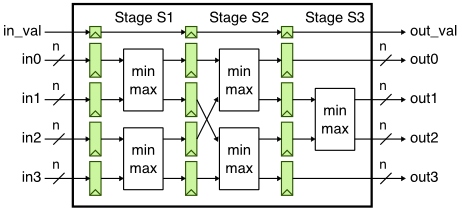
\includegraphics[width=\textwidth]{images/8.png}
\end{figure}
Set your workspace as \texttt{TOP\_DIR} first. The PyMTL3 build files are provided in \texttt{/home/users/\\
ece481/lab6}. Copy it to your \texttt{TOP\_DIR}.
\subsection{Using Synopsys VCS for 4-state RTL simulation}
Using the PyMTL simulation framework can give us a good foundation in verifying a design. However, the PyMTL RTL simulation that you may be accustomed to in ECE 4750 is only a 2-state simulation, meaning a signal can only be 0 or 1. An alternative form of RTL simulation is a 4-state simulation, in which signals can be 0, 1, x, or z.

It is important to note a key difference between 2-state and 4-state simulations. In the 2-state simulation, each variable is initialized to a determined value. This initial condition assumption may or may not be what happens in actual silicon! As a result, a different initial condition could introduce a bug that was not caught by our PyMTL3 2-state RTL simulation. In 4-state simulations, no such assumptions are made. Instead, every signal begins as \texttt{x} and only resolves to a 0 or 1 after it is driven or resolved using x-propagation.
\begin{minted}{verilog}
always @(*)
begin
  if ( control_signal )
    // set signal "signal_a", but bug causes chip to fail
  else
    // set signal "signal_a" such that everything works fine
end
\end{minted}
Look at the above pseudocode. If control\_signal is not reset, then in the 2-state simulation, if you initialize all states to zero, it will look like the chip works fine, but this is not a safe assumption! The real chip does not guarantee that all state is initialized to zero, so we can model that in four state simulation as an x. Since the control signal could initialize to 1, this could non-deterministically cause the chip to fail! What you would see in simulation is that signal\_a would become an \texttt{x} because we do not know the value of control\_signal on reset. This x is propagated through the design, and some simulators are more optimistic/pessimistic about x’s than others. For example, a pessimistic simulator may just assume that any piece of logic that has an x on the input and outputs an x. This is pessimistic because it is possible that you can still resolve the output (imagine a mux where two inputs are the same, but the select bit is an x). Optimism is the opposite, resolving signals to 0 or 1 that should remain an x.

You may notice in your designs that you are passing all 2-state simulations but fail every 4-state simulation. Oftentimes the key to this is that an output is an x for some cycle, which is a good sign you are not handling reset properly. We consider it best practice to force invalid output data to zero to avoid x’s in your 4-state simulation and provide a deterministic output for every cycle, no matter the initial condition.

To create a 4-state simulation, let’s start by creating a build directory for our \texttt{vcs} work.
\begin{minted}{bash}
mkdir -p $TOP_DIR/vcs-rtl-build
cd $TOP_DIR/vcs-rtl-build
\end{minted}
We run \texttt{vcs} to compile a simulation and \texttt{./simv} to run the simulation. Let’s run a 4-state simulation for test\_basic using the design \texttt{SortUnitStructRTL\_\_nbits\_8\_\_pickled.v}.
\begin{minted}[breaklines,breakanywhere]{bash}
vcs ../sim/build/SortUnitStructRTL__nbits_8__pickled.v -full64 -sverilog +incdir+../sim/build +lint=all -xprop=tmerge -top SortUnitStructRTL__nbits_8_tb ../sim/build/SortUnitStructRTL__nbits_8_test_basic_tb.v +vcs+dumpvars+SortUnitStructRTL__nbits_8_test_basic_vcs.vcd -override_timescale=1ns/1ns
./simv
\end{minted}
Synopsys VCS is an extremely in-depth tool with many command-line options. If you want to learn more on your own about other options that are available to you with VCS, you can visit the course webpage here. However, we’ve detailed some of the key command line options below:
\begin{minted}[breaklines,breakanywhere]{text}
../sim/build/SortUnitStructRTL__nbits_8__pickled.v -The path to the source RTL file
-sverilog -Indicates that we are using SystemVerilog
+incdir+../sim/build -Specifies directories that contain files that are tagged with `include. We include ../sim/build because our VTB includes a _tb.v.cases file located within the ../../sim/build directory
-xprop=tmerge -Specifies that we want to use the tmerge truth table for x-propagation (see VCS user manual for more info)
-top SortUnitStructRTL__nbits_8_tb -Indicates the name of the top module (located within the VTB)
../sim/build/SortUnitStructRTL__nbits_8_test_basic_tb.v -The path to the source testbench file
+define+<macro> -defines a macro that may be used in your Verilog code or testbench
+vcs+dumpvars+<filename>.vcd -Tells VCS to dump a VCD in the current dir with the name <filename>.vcd
-override_timescale=1ns/1ns -Changes the timescale. Units/precision
\end{minted}
Let’s run another 4-state simulation, this time using the testbench from the sort-rtl simulator run that the TA ran earlier. Note that while we can use this vcd for power analysis, for the purposes of this lab, we will only be doing power analysis on the final gate-level netlist.% that we’ll obtain from Cadence Innovus.
\begin{minted}[breaklines,breakanywhere]{bash}
vcs ../sim/build/SortUnitStructRTL__nbits_8__pickled.v -full64 -sverilog +incdir+../sim/build +lint=all -xprop=tmerge -top SortUnitStructRTL__nbits_8_tb ../sim/build/SortUnitStructRTL__nbits_8_sort-rtl-struct-random_tb.v +vcs+dumpvars+SortUnitStructRTL__nbits_8_sort-rtl-struct-random_vcs.vcd -override_timescale=1ns/1ns
./simv
\end{minted}
\subsection{(Optional) Using Synopsys Design Compiler for Synthesis}
We use Synopsys Design Compiler (DC) to synthesize Verilog RTL models into a gate-level netlist where all of the gates are from the standard cell library. So Synopsys DC will synthesize the Verilog + operator into a specific arithmetic block at the gate level. Based on various constraints, it may synthesize a ripple-carry adder, a carry-look-ahead adder, or even more advanced parallel-prefix adders.

We start by creating a subdirectory for our work, and then launching Synopsys DC.
\begin{minted}{bash}
mkdir -p $TOPDIR/synopsys-dc
cd $TOPDIR/synopsys-dc
dc_shell-xg-t
\end{minted}
To make it easier to copy-and-paste commands from this document, we tell Synopsys DC to ignore the prefix \verb|dc_shell>| using the following:
\begin{minted}{text}
 dc_shell> alias "dc_shell>" ""
\end{minted}
There are two important variables we need to set before starting to work in Synopsys DC. The target\_library variable specifies the standard cells that Synopsys DC should use when synthesizing the RTL. The link\_library variable should search the standard cells but can also search other cells (e.g., SRAMs) when trying to resolve references in our design. These other cells are not meant to be available for Synopsys DC to use during synthesis but should be used when resolving references. Including * in the link\_library variable indicates that Synopsys DC should also search all cells inside the design itself when resolving references.
\begin{minted}[breaklines,breakanywhere]{tcl}
set_app_var target_library "$env(ECE4810J_STDCELLS)/stdcells.db"
set_app_var link_library "* $env(ECE4810J_STDCELLS)/stdcells.db"
\end{minted}
Note that we can use \texttt{\$env(ECE4810J\_STDCELLS)} to get access to the \texttt{\$ECE4810J\_STDCELLS} environment variable, which specifies the directory containing the standard cells, and that we are referencing the abstract logical and timing views in the .db format.

As an aside, if you want to learn more about any command in any Synopsys tool, you can simply type \texttt{man toolname} at the shell prompt. We are now ready to read the Verilog file, which contains the top-level design and all referenced modules. We do this with two commands. The analyze command reads the Verilog RTL into an intermediate internal representation. The elaborate command recursively resolves all of the module references starting from the top-level module and also infers various registers and/or advanced data-path components.
\begin{minted}[breaklines,breakanywhere]{tcl}
analyze -format sverilog ../sim/build/SortUnitStructRTL__nbits_8__pickled.v
elaborate SortUnitStructRTL__nbits_8
\end{minted}
We need to create a clock constraint to tell Synopsys DC what our target cycle time is. Synopsys DC will not synthesize a design to run “as fast as possible”. Instead, the designer gives Synopsys DC a target cycle time, and the tool will try to meet this constraint while minimizing area and power. The create\_clock command takes the name of the clock signal in the Verilog (which in this course will always be \texttt{clk}), the label to give this clock (i.e., ideal\_clock1), and the target clock period in nanoseconds. So in this example, we are asking Synopsys DC to see if it can synthesize the design to run at 3.33GHz (i.e., a cycle time of 300ps).
\begin{minted}[breaklines,breakanywhere]{text}
dc_shell> create_clock clk -name ideal_clock1 -period 0.3
\end{minted}
In an ideal world, all inputs and outputs would change immediately with the clock edge. In reality, this is not the case. We need to include reasonable delays for inputs and outputs, so Synopsys DC can factor this into its timing analysis so we would still meet timing if we were to tape our design out in real silicon. Here, we choose 5\% of the clock period for our input and output delays.
\begin{minted}[breaklines,breakanywhere]{tcl}
set_input_delay -clock ideal_clock1 [expr 0.3*0.05] [all_inputs]
set_output_delay -clock ideal_clock1 [expr 0.3*0.05] [all_outputs]
\end{minted}
Next, we give Synopsys DC some constraints about fanout and transition slew. Fanout roughly describes the number of inputs driven by a particular output, and the higher the fanout, the higher the drive strength required. Slew rate is how quickly a signal can make a full transition. We want all of our signals to meet a good slew, meaning that they can transition quickly, so we set the maximum slew to one-quarter of the clock period.
\begin{minted}[breaklines,breakanywhere]{tcl}
set_max_fanout 20 SortUnitStructRTL__nbits_8
set_max_transition [expr 0.25*0.3] SortUnitStructRTL__nbits_8
\end{minted}
We can use the \texttt{check\_design} command to make sure there are no obvious errors in our Verilog RTL.
\begin{minted}{text}
dc_shell> check_design
\end{minted}
You may see some warnings regarding clk[0] and reset[0] ports not being connected to any nets in certain modules. This is OK, since in PyMTL translation, we automatically add those ports to all modules, so they may not actually be used. Aside from this, you should not see any warnings. However, it is critical that you carefully review all warnings and errors when you analyze and elaborate a design with Synopsys DC. There may be many warnings, but you should still skim through them. Often times there will be something very wrong in your Verilog RTL which means any results from using the ASIC tools is completely bogus. Synopsys DC will output a warning, but Synopsys DC will usually just keep going, potentially producing a completely incorrect gate-level model!

Finally, the \texttt{compile} command will do the synthesis.
\begin{minted}{text}
dc_shell> compile
\end{minted}
During synthesis, Synopsys DC will display information about its optimization process. It will report on its attempts to map the RTL into standard cells, optimize the resulting gate-level netlist to improve the delay, and then optimize the final design to save area.

The \texttt{compile} command does not \textit{flatten} your design. Flatten means to remove module hierarchy boundaries; so instead of having module A and module B within module C, Synopsys DC will take all of the logic in module A and module B and put it directly in module C. You can enable flattening with the \texttt{-ungroup\_all} option. Without extra hierarchy boundaries, Synopsys DC is able to perform more optimizations and potentially achieve better area, energy, and timing. However, an unflattened design is much easier to analyze since if there is a module A in your RTL design, that same module will always be in the synthesized gate-level netlist.

The \texttt{compile} command does not perform many optimizations. Synopsys DC also includes \texttt{compile\_ultra}, which does many more optimizations and will likely produce higher-quality of results. Keep in mind that the \texttt{compile} command will \textit{not} flatten your design by default, while the \texttt{compile\_ultra} command \textit{will} flatten your design by default. You can turn off flattening by using the \texttt{-no\_autoungroup} option with the \texttt{compile\_ultra} command. \texttt{compile\_ultra} also has the option \texttt{-gate\_clock}, which automatically performs clock gating on your design, which can save quite a bit of power. Once you finish this part, feel free to go back and experiment with the \texttt{compile\_ultra} command.

Now that we have synthesized the design, we output the resulting gate-level netlist in two different file formats: Verilog and .ddc (which we will use with Synopsys DesignVision). We also output a .sdc file which contains the constraint information we gave Synopsys. We will pass this same constraint information to Cadence Innovus during the place and route portion of the flow.
\begin{minted}{tcl}
write -format verilog -hierarchy -output post-synth.v
write -format ddc     -hierarchy -output post-synth.ddc
write_sdc -nosplit post-synth.sdc
\end{minted}
We can use various commands to generate reports about the area, energy, and timing. The \texttt{report\_timing} command will show the critical path through the design. Part of the report is displayed below. Note that this report was generated using a clock constraint of 300ps.
\begin{minted}[breaklines,breakanywhere]{text}
dc_shell> report_timing -nosplit -transition_time -nets -attributes
  ...
  Point                                       Fanout     Trans      Incr       Path      Attributes
  ---------------------------------------------------------------------------------------------------------
  clock ideal_clock1 (rise edge)                                    0.00       0.00
  clock network delay (ideal)                                       0.00       0.00

  elm_S2S3__1/out_reg[5]/Q (DFF_X1)                       0.01      0.08       0.08 f
  elm_S2S3__1/out[5] (net)                      2                   0.00       0.08 f
  elm_S2S3__1/out[5] (Reg__Type_Bits8_3)                            0.00       0.08 f
  elm_S2S3__out[1][5] (net)                                         0.00       0.08 f
  minmax_S3/in0[5] (MinMaxUnit__nbits_8_1)                          0.00       0.08 f
  minmax_S3/in0[5] (net)                                            0.00       0.08 f
  minmax_S3/U13/ZN (INV_X1)                               0.01      0.02       0.11 r
  minmax_S3/n11 (net)                           1                   0.00       0.11 r
  minmax_S3/U12/ZN (OR2_X1)                               0.01      0.03       0.14 r
  minmax_S3/n30 (net)                           1                   0.00       0.14 r
  minmax_S3/U36/ZN (NAND4_X1)                             0.02      0.04       0.18 f
  minmax_S3/n41 (net)                           1                   0.00       0.18 f
  minmax_S3/U40/ZN (OAI221_X1)                            0.05      0.06       0.24 r
  minmax_S3/n45 (net)                           3                   0.00       0.24 r
  minmax_S3/U9/ZN (AND2_X1)                               0.03      0.08       0.32 r
  minmax_S3/n9 (net)                            5                   0.00       0.32 r
  minmax_S3/U47/Z (MUX2_X1)                               0.01      0.08       0.40 f
  minmax_S3/out_min[0] (net)                    1                   0.00       0.40 f
  minmax_S3/out_min[0] (MinMaxUnit__nbits_8_1)                      0.00       0.40 f
  minmax_S3__out_min[0] (net)                                       0.00       0.40 f
  U61/ZN (AND2_X1)                                        0.01      0.03       0.43 f
  out[1][0] (net)                               1                   0.00       0.43 f
  out[1][0] (out)                                         0.01      0.00       0.43 f
  data arrival time                                                            0.43

  clock ideal_clock1 (rise edge)                                    0.30       0.30
  clock network delay (ideal)                                       0.00       0.30
  output external delay                                            -0.01       0.29
  data required time                                                           0.29
  ---------------------------------------------------------------------------------------------------------
  data required time                                                           0.29
  data arrival time                                                           -0.43
  ---------------------------------------------------------------------------------------------------------
  slack (VIOLATED)                                                            -0.15
\end{minted}
This timing report uses static timing analysis to find the critical path. Static timing analysis checks the timing across all paths in the design (regardless of whether these paths can actually be used in practice) and finds the longest path. The report clearly shows that the critical path starts at bit 5 of a pipeline register in between the S1 and S2 stages (elm\_S0S1\_\_0), goes into the first input of a MinMaxUnit, comes out the out\_min port of the MinMaxUnit, and ends at a pipeline register in between the S1 and S2 stages (elm\_S1S2\_\_0). The report shows the delay through each logic gate (e.g., the \texttt{clk-to-q} delay of the initial DFF is 90ps, the propagation delay of a NAND2\_X1 gate is 30ps) and the total delay for the critical path, which in this case is 0.38ns. Notice that there are two NAND2\_X1 gates, but they do have the same propagation delay; this is because the static timing analysis also factors in input slew rates, rise vs. fall time, and output load when calculating the delay of each gate. We set the clock constraint to be 300ps, but also notice that the report factors in the setup time required at the final register. The setup time is 40ps, so in order to operate the sort unit at 1ns and meet the setup time, we would need the critical path to arrive at 260ps.

The difference between the required arrival time and the actual arrival time is called \textit{slack}. Positive slack means the path arrived before it needed to while negative slack means the path arrived after it needed to. If you end up with negative slack, then you need to rerun the tools with a longer target clock period until you can meet timing with no negative slack. The process of tuning a design to ensure it meets timing is called “timing closure”. In this lab, we are primarily interested in design-space exploration as opposed to meeting some externally defined target timing specifications. So you will need to sweep a range of target clock periods. Our goal is to choose the shortest possible clock period which still meets timing without any negative slack! This will result in a well-optimized design and help identify the “fundamental” performance of the design. Alternatively, if you are comparing multiple designs, sometimes the best situation is to tune the baseline so it has a couple of percent of negative slack and then ensure the alternative designs have similar cycle times. This will enable a fair comparison since all designs will be running at the same cycle time.

The \texttt{report\_area} command can show how much area each module uses and can enable detailed area breakdown analysis.
\begin{minted}[breaklines,breakanywhere]{text}
dc_shell> report_area -nosplit -hierarchy
...
Combinational area:                393.414001
Buf/Inv area:                       92.301999
Noncombinational area:             453.795984
Macro/Black Box area:                0.000000
Net Interconnect area:      undefined  (Wire load has zero net area)

Total cell area:                   847.209985
Total area:                 undefined

Hierarchical area distribution
------------------------------

                                  Global cell area          Local cell area
                                  ------------------  ---------------------------
Hierarchical cell                 Absolute   Percent  Combi-    Noncombi-  Black-
                                  Total      Total    national  national   boxes   Design
--------------------------------  ---------  -------  --------  ---------  ------  -----------------------------------
  SortUnitStructRTL__nbits_8
elm_S0S1__0                         36.1760      4.3    0.0000    36.1760  0.0000  Reg__Type_Bits8_0
elm_S0S1__1                         36.1760      4.3    0.0000    36.1760  0.0000  Reg__Type_Bits8_11
elm_S0S1__2                         36.1760      4.3    0.0000    36.1760  0.0000  Reg__Type_Bits8_10
elm_S0S1__3                         36.1760      4.3    0.0000    36.1760  0.0000  Reg__Type_Bits8_9
elm_S1S2__0                         36.1760      4.3    0.0000    36.1760  0.0000  Reg__Type_Bits8_8
elm_S1S2__1                         36.1760      4.3    0.0000    36.1760  0.0000  Reg__Type_Bits8_7
elm_S1S2__2                         36.7080      4.3    0.0000    36.7080  0.0000  Reg__Type_Bits8_6
elm_S1S2__3                         36.7080      4.3    0.0000    36.7080  0.0000  Reg__Type_Bits8_5
elm_S2S3__0                         37.2400      4.4    0.0000    37.2400  0.0000  Reg__Type_Bits8_4
elm_S2S3__1                         36.1760      4.3    0.0000    36.1760  0.0000  Reg__Type_Bits8_3
elm_S2S3__2                         38.5700      4.6    0.0000    38.5700  0.0000  Reg__Type_Bits8_2
elm_S2S3__3                         37.7720      4.5    0.0000    37.7720  0.0000  Reg__Type_Bits8_1
minmax0_S1                          70.7560      8.4   70.7560     0.0000  0.0000  MinMaxUnit__nbits_8_0
minmax0_S2                          71.2880      8.4   71.2880     0.0000  0.0000  MinMaxUnit__nbits_8_4
minmax1_S1                          71.8200      8.5   71.8200     0.0000  0.0000  MinMaxUnit__nbits_8_3
minmax1_S2                          71.2880      8.4   71.2880     0.0000  0.0000  MinMaxUnit__nbits_8_2
minmax_S3                           67.0320      7.9   67.0320     0.0000  0.0000  MinMaxUnit__nbits_8_1
val_S0S1                             5.8520      0.7    1.3300     4.5220  0.0000  RegRst__Type_Bits1__reset_value_0_0
val_S1S2                             5.8520      0.7    1.3300     4.5220  0.0000  RegRst__Type_Bits1__reset_value_0_2
val_S2S3                             5.8520      0.7    1.3300     4.5220  0.0000  RegRst__Type_Bits1__reset_value_0_1
--------------------------------  ---------  -------  --------  ---------  ------  -----------------------------------
Total                                                 393.4140   453.7960  0.0000
\end{minted}
The units are in square microns. The cell area can sometimes be different from the total area. The total cell area includes just the standard cells, while the total area can include interconnect area as well. If available, we will want to use the total area in our analysis. Otherwise, we can just use the cell area. So we can see that the sort unit consumes approximately $847\mu \text{m}^2$ of area. We can also see that each pipeline register consumes about 4-5\% of the area, while the MinMaxUnits consume about $\sim$40\% of the area. This is one reason we try not to flatten our designs since the module hierarchy helps us understand the area breakdowns. If we completely flattened the design, there would only be one line in the above table.

The \texttt{report\_power} command can show how much power each module consumes. Note that this power analysis is actually not that useful yet, since at this stage of the flow, the power analysis is based purely on statistical activity factor estimation. Basically, Synopsys DC assumes every net toggles 10\% of the time. This is a pretty poor estimate, so we should never use this kind of statistical power estimation in this lab.
\begin{minted}[breaklines,breakanywhere]{text}
dc_shell> report_power -nosplit -hierarchy
\end{minted}
Finally, we go ahead and exit Synopsys DC.
\begin{minted}{text}
dc_shell> exit
\end{minted}
Take a few minutes to examine the resulting Verilog gate-level netlist. Notice that the module hierarchy is preserved and also notice that the MinMaxUnit synthesizes into a large number of basic logic gates.
\begin{minted}{bash}
cd $TOPDIR/synopsys-dc
more post-synth.v
\end{minted}
We can use the Synopsys Design Vision (DV) tool for browsing the resulting gate-level netlist, plotting critical path histograms, and generally analyzing our design. Start Synopsys DV and setup the target\_library and link\_library variables as before.
\begin{minted}[breaklines,breakanywhere]{text}
% cd $TOPDIR/synopsys-dc
% design_vision-xg
design_vision> set_app_var target_library "$env(ECE4810J_STDCELLS)/stdcells.db"
design_vision> set_app_var link_library "* $env(ECE4810J_STDCELLS)/stdcells.db"
\end{minted}
Choose File > Read from the menu to open post-synth.ddc file generated during synthesis. You can then use the following steps to view the gate-level schematic for the MinMaxUnit:
\begin{itemize}
    \item Select the minmax0\_S1 module in the Logical Hierarchy panel
    \item Choose \textit{Schematic > New Schematic View} from the menu
    \item Double-click the box representing the MinMaxUnit in the schematic view
\end{itemize}
\begin{figure}[H]
    \centering
    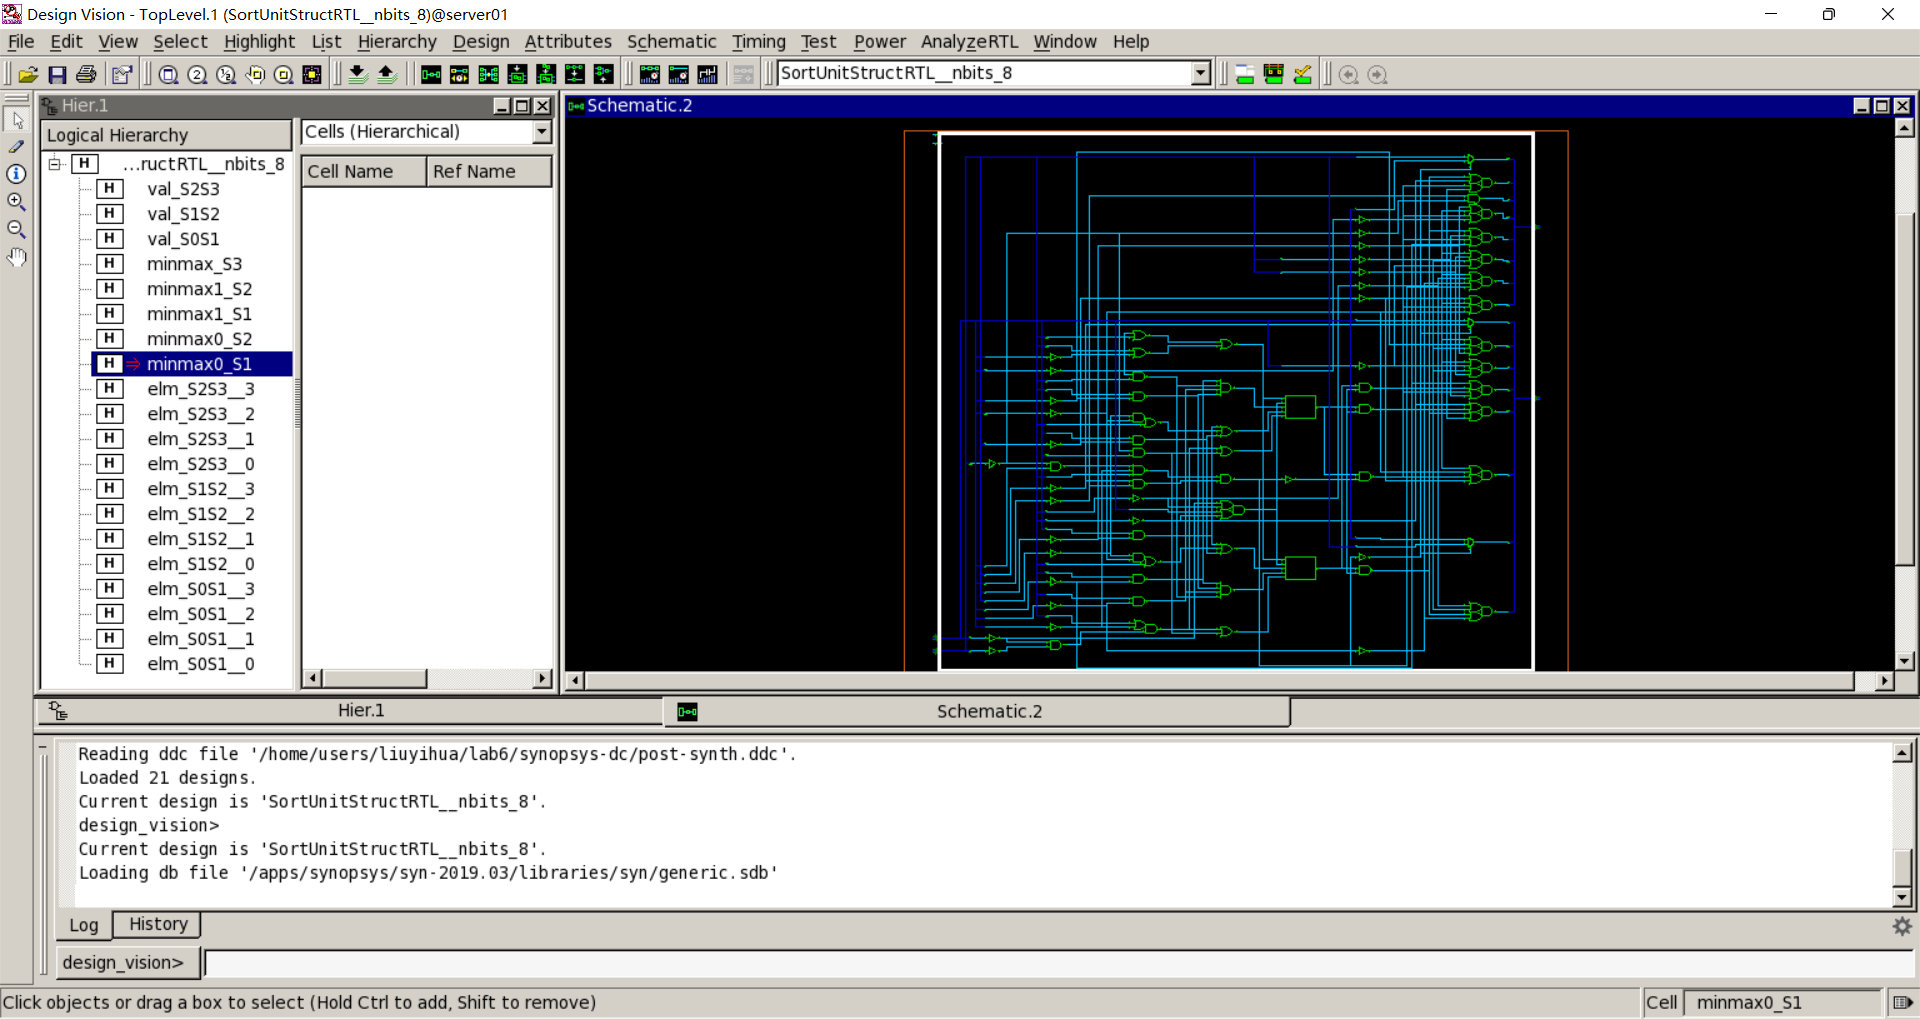
\includegraphics[width=\textwidth]{images/9.png}
\end{figure}
This shows you the exact gates used to implement the MinMaxUnit. You can use the following steps to view a histogram of path slack and also to open a gave-level schematic of just the critical path.
\begin{itemize}
    \item Choose \textit{Timing > Path Slack} from the menu
    \item Click \textit{OK} in the pop-up window
    \item Select the left-most bar in the histogram to see the list of the most critical paths
    \item Right click first path (the critical path) and choose \textit{Path Schematic}
\end{itemize}
\begin{figure}[H]
    \centering
    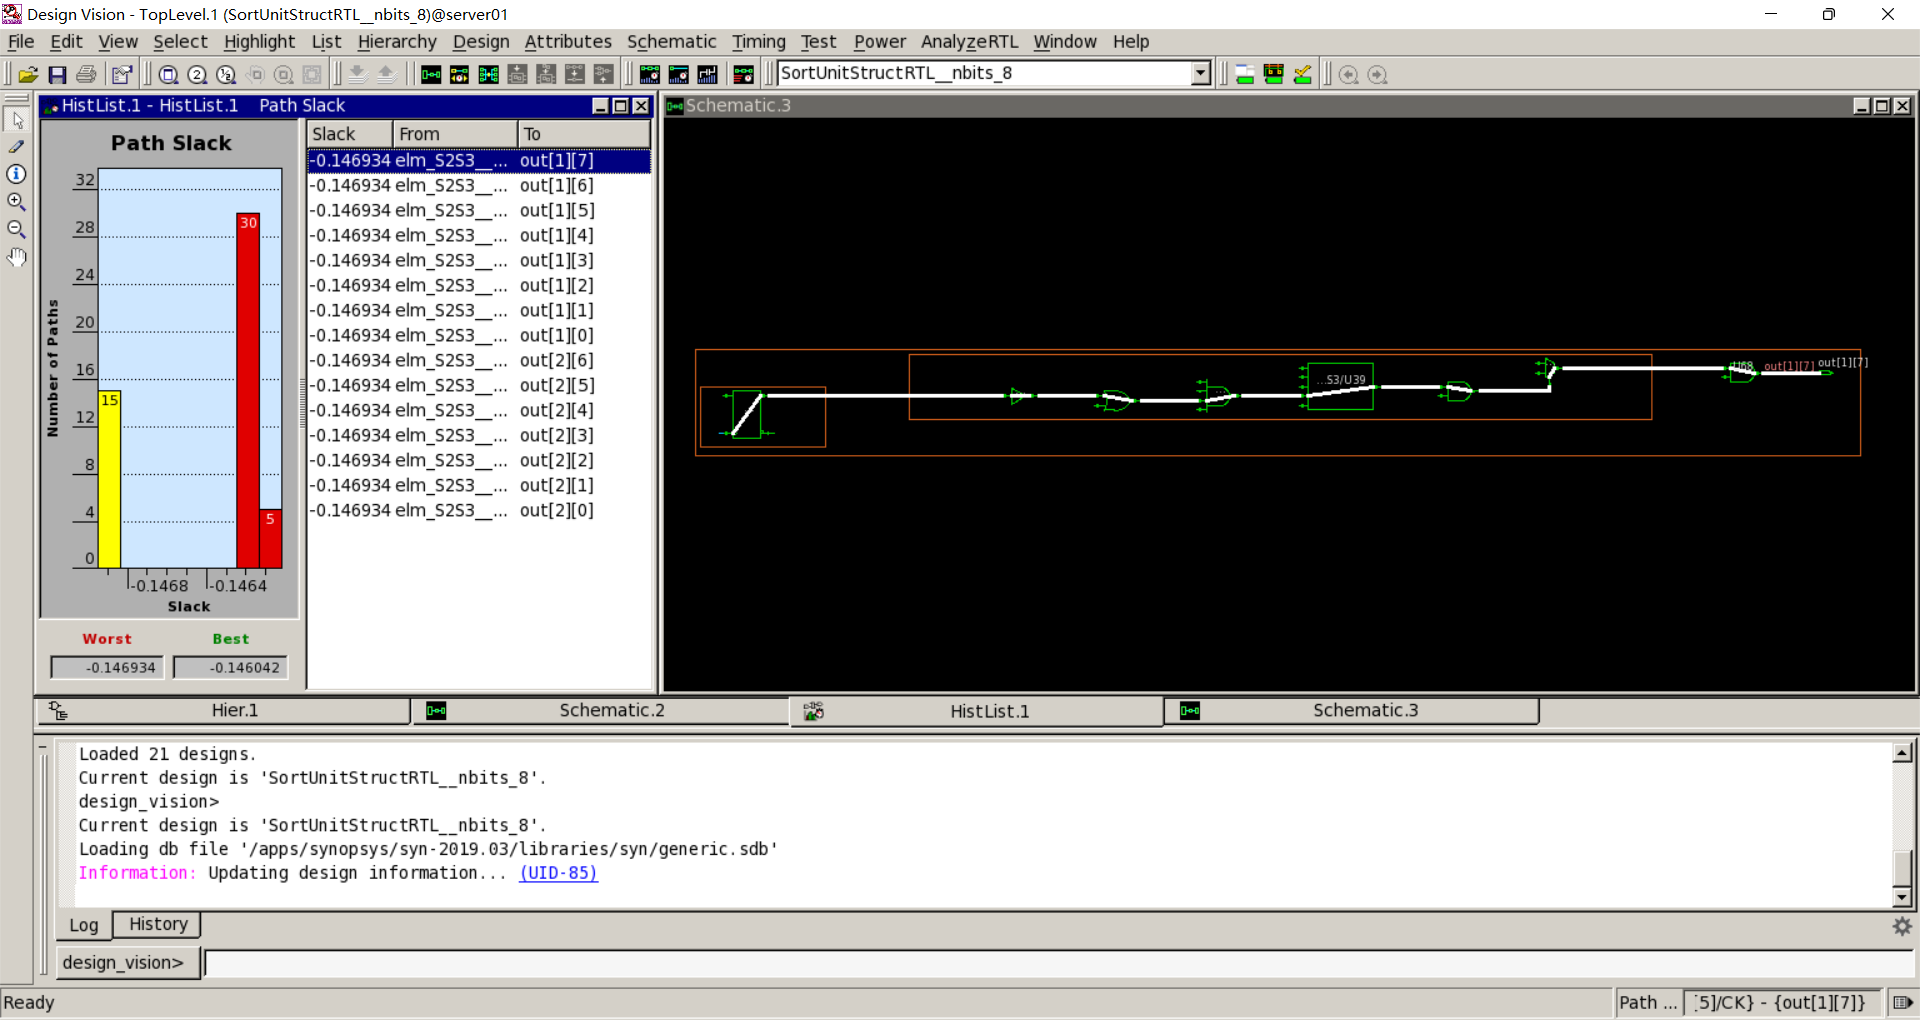
\includegraphics[width=\textwidth]{images/10.png}
\end{figure}
This shows you the exact gates that lie on the critical path. Notice that there are nine levels of logic (including the registers) on the critical path. The number of levels of logic on the critical path can provide some very rough first-order intuition on whether or not we might want to explore a more aggressive clock constraint and/or add more pipeline stages. If there are just a few levels of logic on the critical path, then our design is probably very simple (as in this case!), while if there are more than 50 levels of logic, then there is potentially room for significant improvement. The screen capture above illustrates using Design Vision to explore the post-synthesis results. While this can be interesting, in this lab, we almost always prefer exploring the post-place-and-route results, so we will not really use Synopsys DC that often.

\textbf{To Do On Your Own}: Sweep a range of target clock frequencies to determine the shortest possible clock period which still meets timing without any negative slack. You can put a sequence of commands in a .tcl file and then run Synopsys DC using those commands in one step like this:
\begin{minted}[breaklines,breakanywhere]{bash}
cd $TOPDIR/synopsys-dc
dc_shell-xg-t -f init.tcl
\end{minted}
So consider placing the commands from this section into a .tcl file and then running Synopsys DC with a target clock period of 0.3ns. Then gradually increase the clock period until your design meets timing. To follow along with the lab, push the design through synth again using 0.6 ns as your clock constraint, as this is what we will be using for the rest of the flow.

For the correct timing report and area report, see Appendix \ref{ADC}.
\subsection{Using Synopsys VCS for Fast Functional Gate-Level Simulation}
Before synthesis, we used Synopsys VCS to do a 4-state simulation. This time, we’ll be using VCS to perform a gate-level simulation since we now have a gate-level netlist available to us. Gate-level simulation provides an advantage over RTL simulation because it more precisely represents the specification of the true hardware generated by the tools. This sort of simulation could propagate X’s into the design that was not found by the 4-state RTL simulation, and it also verifies that the tools did not optimize anything away during synthesis. A fast-functional simulation is a zero-delay simulation that provides a way to check functionality at the gate level without worrying about the timing checks involved in a back-annotated gate-level simulation, which we will perform later in this lab.
\begin{minted}[breaklines,breakanywhere]{bash}
mkdir -p $TOPDIR/vcs-postsyn-build
cd $TOPDIR/vcs-postsyn-build
\end{minted}
Then we’ll run \texttt{vcs} and ./simv to run our gate-level simulation on the sort-rtl-struct-random simulator testbench:
\begin{minted}[breaklines,breakanywhere]{bash}
vcs ../synopsys-dc/post-synth.v $ECE4810J_STDCELLS/stdcells.v -full64 -sverilog +incdir+../sim/build +lint=all -xprop=tmerge -top SortUnitStructRTL__nbits_8_tb ../sim/build/SortUnitStructRTL__nbits_8_sort-rtl-struct-random_tb.v +define+CYCLE_TIME=0.6 +define+VTB_INPUT_DELAY=0.03 +define+VTB_OUTPUT_ASSERT_DELAY=0.57 +delay_mode_zero +vcs+dumpvars+SortUnitStructRTL__nbits_8_sort-rtl-struct-random_vcs.vcd -override_timescale=1ns/1ps
./simv
\end{minted}
Notice there are some differences in the \texttt{vcs} command we ran here and the one we ran for the 4-state RTL simulation. In this version, we use the gate-level netlist \texttt{post-synth.v} instead of the pickled file. We also include the option \texttt{+delay\_mode\_zero}, which tells VCS to run a fast-functional simulation in which no delays are considered. This is similar to RTL simulation, and you should notice that all signals will change on the clock edge. We also include the macros \texttt{CYCLE\_TIME}, \texttt{VTB\_INPUT\_DELAY}, \texttt{VTB\_OUTPUT\_ASSERT\_DELAY}. These values are not actually critical for a fast-functional simulation, but we set them to the same values as the Back-Annotated gate-level simulations to make comparing VCDs easier when debugging.
\subsection{Using Cadence Innovus for Place-and-Route}
We use Cadence Innovus for placing standard cells in rows and then automatically routing all of the nets between these standard cells. We also use Cadence Innovus to route the power and ground rails in a grid and connect this grid to the power and ground pins of each standard cell, and to automatically generate a clock tree to distribute the clock to all sequential state elements with hopefully low skew.

We will be running Cadence Innovus in a separate directory to keep the files separate from the other tools.
\begin{minted}{bash}
mkdir -p $TOPDIR/cadence-innovus
cd $TOPDIR/cadence-innovus
\end{minted}
Before starting Cadence Innovus, we need two files that will be loaded into the tool. The first file is a .sdc file which contains timing constraint information about our design. This file is where we specify our target clock period, but it is also where we could specify input or output delay constraints (e.g., the output signals must be stable 200ps before the rising edge). We created this file at the end of our synthesis step using Synopsys DC. Before we get started, let’s open that file to take a look at the constraint DC generated.
\begin{minted}{bash}
less ../synopsys-dc/post-synth.sdc
\end{minted}
The \texttt{create\_clock} command is similar to the command we used in synthesis, and we usually use the same target clock period that we used for synthesis. In this case, we are targeting a 1.67GHz clock frequency (i.e., a 0.6ns clock period). Note that we also see the constraints that we set for input and output delay, max fanout, max transition, as well as our path groups.

The second file is a “multi-mode multi-corner” (MMMC) analysis file. This file specifies what “corner” to use for our timing analysis. A corner is a characterization of the standard cell library and technology with specific assumptions about the process, temperature, and voltage (PVT). So we might have a “fast” corner which assumes best-case process variability, low temperature, and high voltage, or we might have a “slow” corner which assumes worst-case variability, high temperature, and low voltage. To ensure our design will work across a range of operating conditions, we need to evaluate our design across a range of corners. In this course, we will keep things simple by only considering a “typical” corner (i.e., average PVT). Use Geany or your favorite text editor to create a file named \texttt{setup-timing.tcl} in \texttt{\$TOPDIR/cadence-innovus} with the following content:
\begin{minted}[breaklines]{tcl}
create_rc_corner -name typical -cap_table "$env(ECE4810J_STDCELLS)/rtk-typical.captable" -T 25
create_library_set -name libs_typical -timing [list "$env(ECE4810J_STDCELLS)/stdcells.lib"]
create_delay_corner -name delay_default -early_library_set libs_typical -late_library_set libs_typical -rc_corner typical
create_constraint_mode -name constraints_default -sdc_files [list ../synopsys-dc/post-synth.sdc]
create_analysis_view -name analysis_default -constraint_mode constraints_default -delay_corner delay_default
set_analysis_view -setup [list analysis_default] -hold [list analysis_default]
\end{minted}
The \texttt{create\_rc\_corner} command loads in the .captable file that we examined earlier. This file includes information about the resistance and capacitance of every metal layer. Notice that we are loading in the “typical” captable, and we are specifying an “average” operating temperature of 25 degC. The \texttt{create\_library\_set} command loads in the .lib file that we examined earlier. This file includes information about the input/output capacitance of each pin in each standard cell, along with the delay from every input to every output in the standard cell. The \texttt{create\_delay\_corner} specifies a specific corner that we would like to use for our timing analysis by putting together a .captable and a .lib file. In this specific example, we are creating a typical corner by putting together the typical .captable and typical .lib we just loaded. The \texttt{create\_constraint\_mode} command loads in the .sdc file we mentioned earlier in this section. The \texttt{create\_analysis\_view} command puts together constraints with a specific corner, and the \texttt{set\_analysis\_view} command tells Cadence Innovus that we would like to use this specific analysis view for both setup and hold time analysis.

\textit{In this lab, we will use Cadence Innovus v20.13-s083\_1}. Now that we have created our \texttt{setup-timing.tcl} file, we can start Cadence Innovus:
\begin{minted}{bash}
cd $TOPDIR/cadence-innovus
innovus -64
\end{minted}
As we enter commands, we will be able to use the GUI to see incremental progress toward a fully placed-and-routed design. We need to set various variables before starting to work in Cadence Innovus. These variables tell Cadence Innovus the location of the MMMC file, the location of the Verilog gate-level netlist, the name of the top-level module in our design, the location of the .lef files, and finally, the names of the power and ground nets.
\begin{minted}[breaklines]{tcl}
set init_mmmc_file "setup-timing.tcl"
set init_verilog   "../synopsys-dc/post-synth.v"
set init_top_cell  "SortUnitStructRTL__nbits_8"
set init_lef_file  "$env(ECE4810J_STDCELLS)/rtk-tech.lef $env(ECE4810J_STDCELLS)/stdcells.lef"
set init_gnd_net   "VSS"
set init_pwr_net   "VDD"
\end{minted}
We are now ready to use the \texttt{init\_design} command to read in the Verilog, set the design name, set up the timing analysis views, read the technology .lef for layer information, and read the standard cell .lef for physical information about each cell used in the design.
\begin{minted}{text}
innovus> init_design
\end{minted}
Then, we tell innovus the type of timing analysis we want it to do. In on-chip variation (OCV) mode, the software calculates clock and data path delays based on minimum and maximum operating conditions for setup analysis and vice-versa for hold analysis. These delays are used together in the analysis of each check. The OCV is the small difference in the operating parameter value across the chip. Each timing arc in the design can have an early and a late delay to account for the on-chip process, voltage, and temperature variation. We need this mode in order to do proper hold time fixing later on.
\begin{minted}{text}
innovus> setAnalysisMode -analysisType onChipVariation -cppr both
\end{minted}
The next step is to do some floorplaning. This is where we broadly organize the chip in terms of its overall dimensions and the placement of any previously designed blocks. For now we just do some very simple floorplanning using the floorPlan command.
\begin{minted}{text}
innovus> floorPlan -r 1.0 0.70 4.0 4.0 4.0 4.0
\end{minted}
In this example, we have chosen the aspect ratio to be 1.0 and the target cell utilization to be 70\%. The cell utilization is the percentage of the final chip that will actually contain useful standard cells as opposed to just “filler” cells (i.e., empty cells). Ideally, we would like the cell utilization to be 100\%, but this is simply not reasonable. If the cell utilization is too high, Cadence Innovus will spend way too much time trying to optimize the design and will eventually simply give up. A target cell utilization of 70\% makes it more likely that Cadence Innovus can successfully place and route the design. We have also added 4.0um of margin around the top, bottom, left, and right of the chip to give us room for the power ring, which will go around the entire chip.

The following screen capture illustrates what you should see: a square floorplan with rows where the standard cells will eventually be placed. You can use the View > Fit menu option to see the entire chip.
\begin{figure}[H]
    \centering
    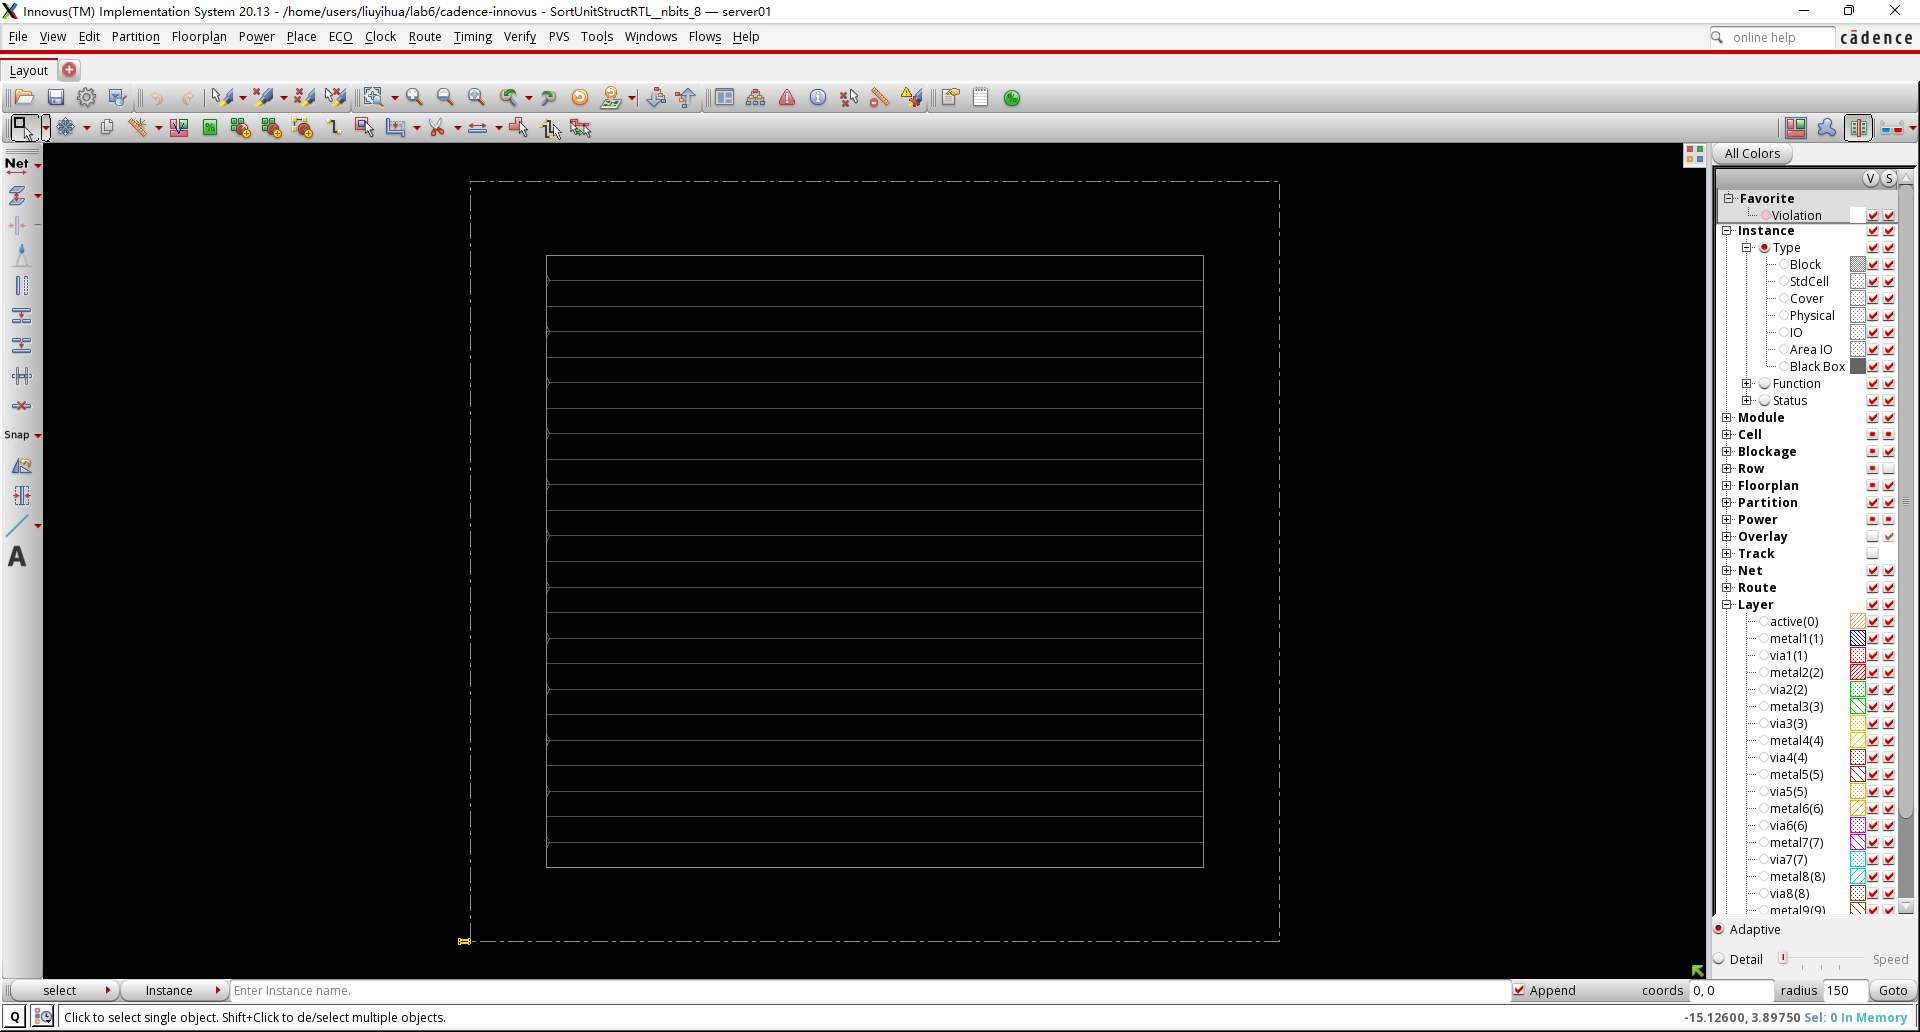
\includegraphics[width=\textwidth]{images/11.png}
\end{figure}
The next step is to work on power routing. Recall that each standard cell has internal M1 power and ground rails which will connect via abutment when the cells are placed into rows. If we were just to supply power to cells using these rails, we would likely have a large IR drop, and the cells in the middle of the chip would effectively be operating at a much lower voltage. During power routing, we create a grid of power and ground wires on the top metal layers and then connect this grid down to the M1 power rails in each row. We also create a power ring around the entire floorplan. Before doing the power routing, we need to use the \texttt{globalNetCommand} command to tell Cadence Innovus which nets are power and which nets are ground (there are \textit{many} possible names for power and ground!).
\begin{minted}[breaklines]{tcl}
globalNetConnect VDD -type pgpin -pin VDD -inst * -verbose
globalNetConnect VSS -type pgpin -pin VSS -inst * -verbose
\end{minted}
We can now draw M1 “rails” for the power and ground rails that go along each row of standard cells.
\begin{minted}{text}
innovus> sroute -nets {VDD VSS}
\end{minted}
We now create a power ring around our chip using the \texttt{addRing} command. A power ring ensures we can easily get power and ground to all standard cells. The command takes parameters specifying the width of each wire in the ring, the spacing between the two rings, and what metal layers to use for the ring. We will put the power ring on M6 and M7; we often put the power routing on the top metal layers since these are fundamentally global routes and these top layers have low resistance, which helps us minimize static IR drop and di/dt noise. These top layers have high capacitance, but this is not an issue since the power and ground rails are not switching (and indeed, this extra capacitance can serve as a very modest amount of decoupling capacitance to smooth out time variations in the power supply).
\begin{minted}[breaklines]{text}
innovus> addRing -nets {VDD VSS} -width 0.6 -spacing 0.5 -layer [list top 7 bottom 7 left 6 right 6]
\end{minted}
\begin{figure}[H]
    \centering
    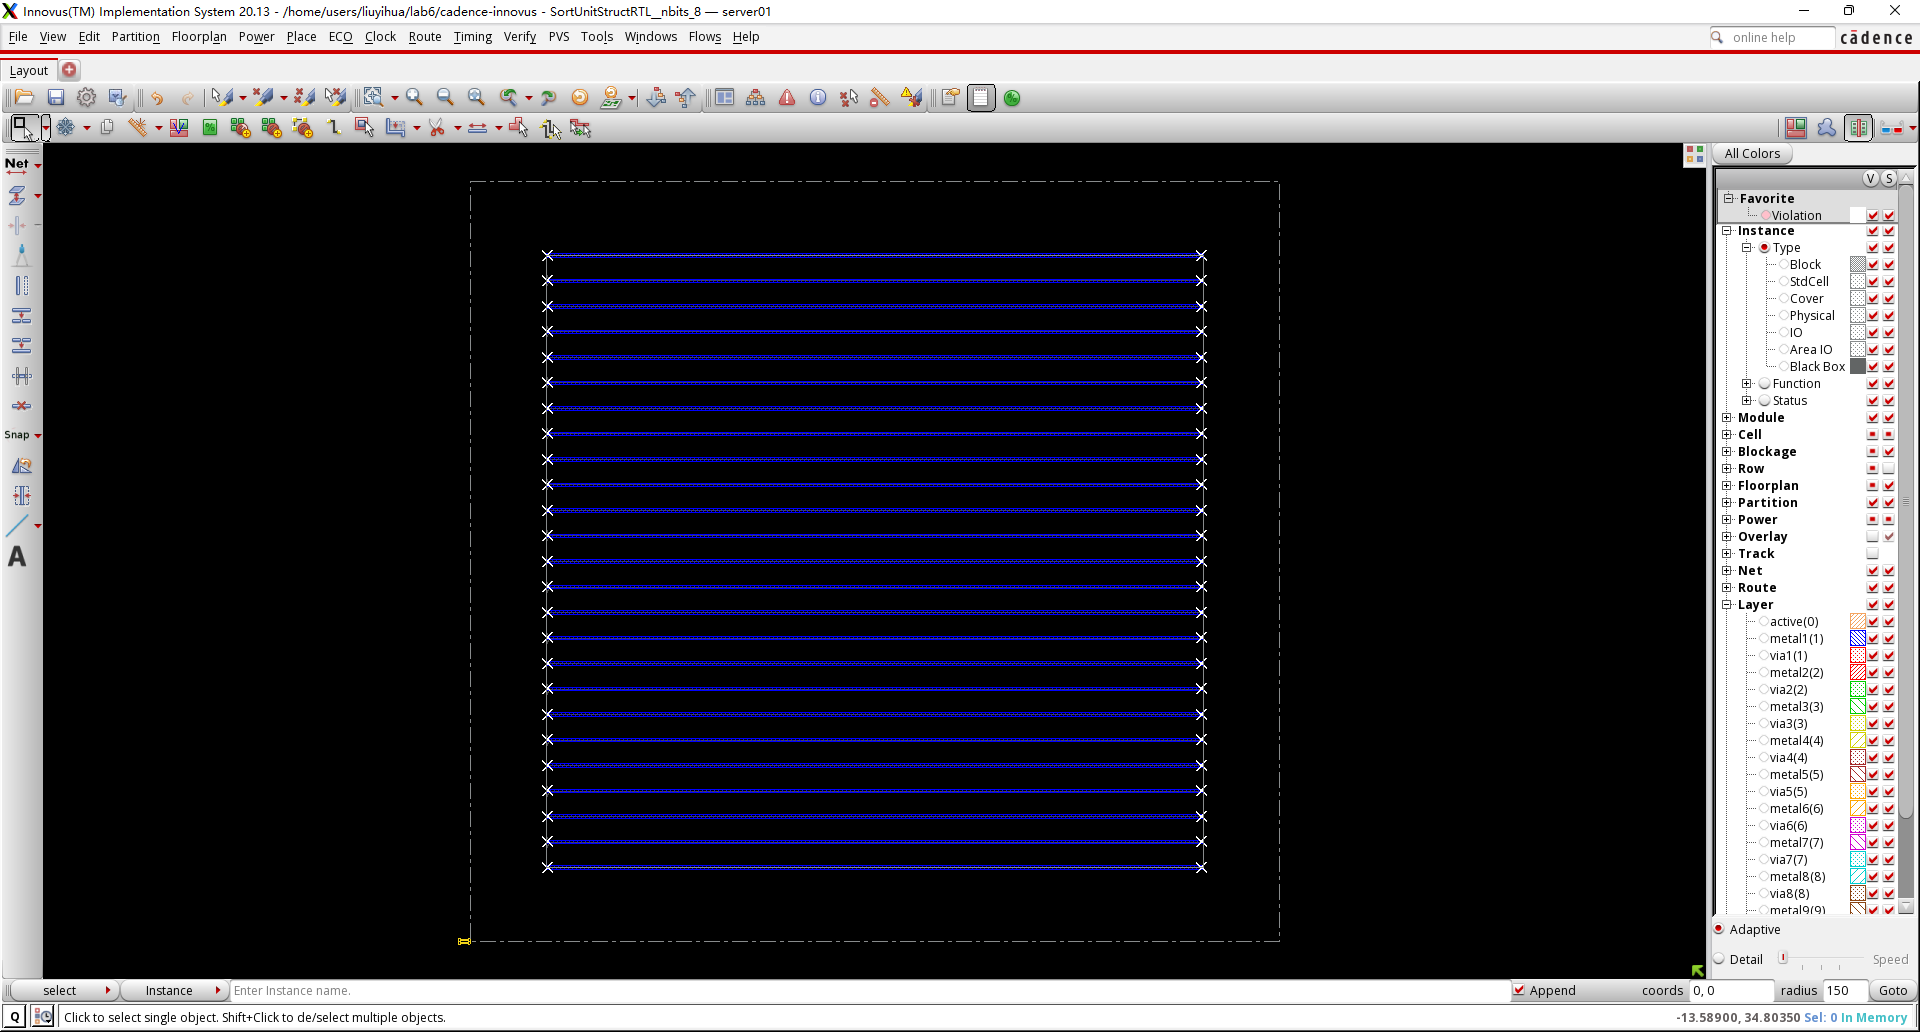
\includegraphics[width=\textwidth]{images/12.png}
\end{figure}
We have power and ground rails along each row of standard cells and a power ring, so now we need to hook these up. We can use the \texttt{addStripe} command to draw wires and automatically insert vias whenever wires cross. First, we draw the vertical “stripes”.
\begin{minted}[breaklines]{text}
innovus> addStripe -nets {VSS VDD} -layer 6 -direction vertical -width 0.4 -spacing 0.5 -set_to_set_distance 5 -start 0.5
\end{minted}
And then, we draw the horizontal “stripes”.
\begin{minted}[breaklines]{text}
innovus> addStripe -nets {VSS VDD} -layer 7 -direction horizontal -width 0.4 -spacing 0.5 -set_to_set_distance 5 -start 0.5
\end{minted}
The following screen capture illustrates what you should see: a power ring and grid on M6 and M7 connected to the horizontal power and ground rails on M1.
\begin{figure}[H]
    \centering
    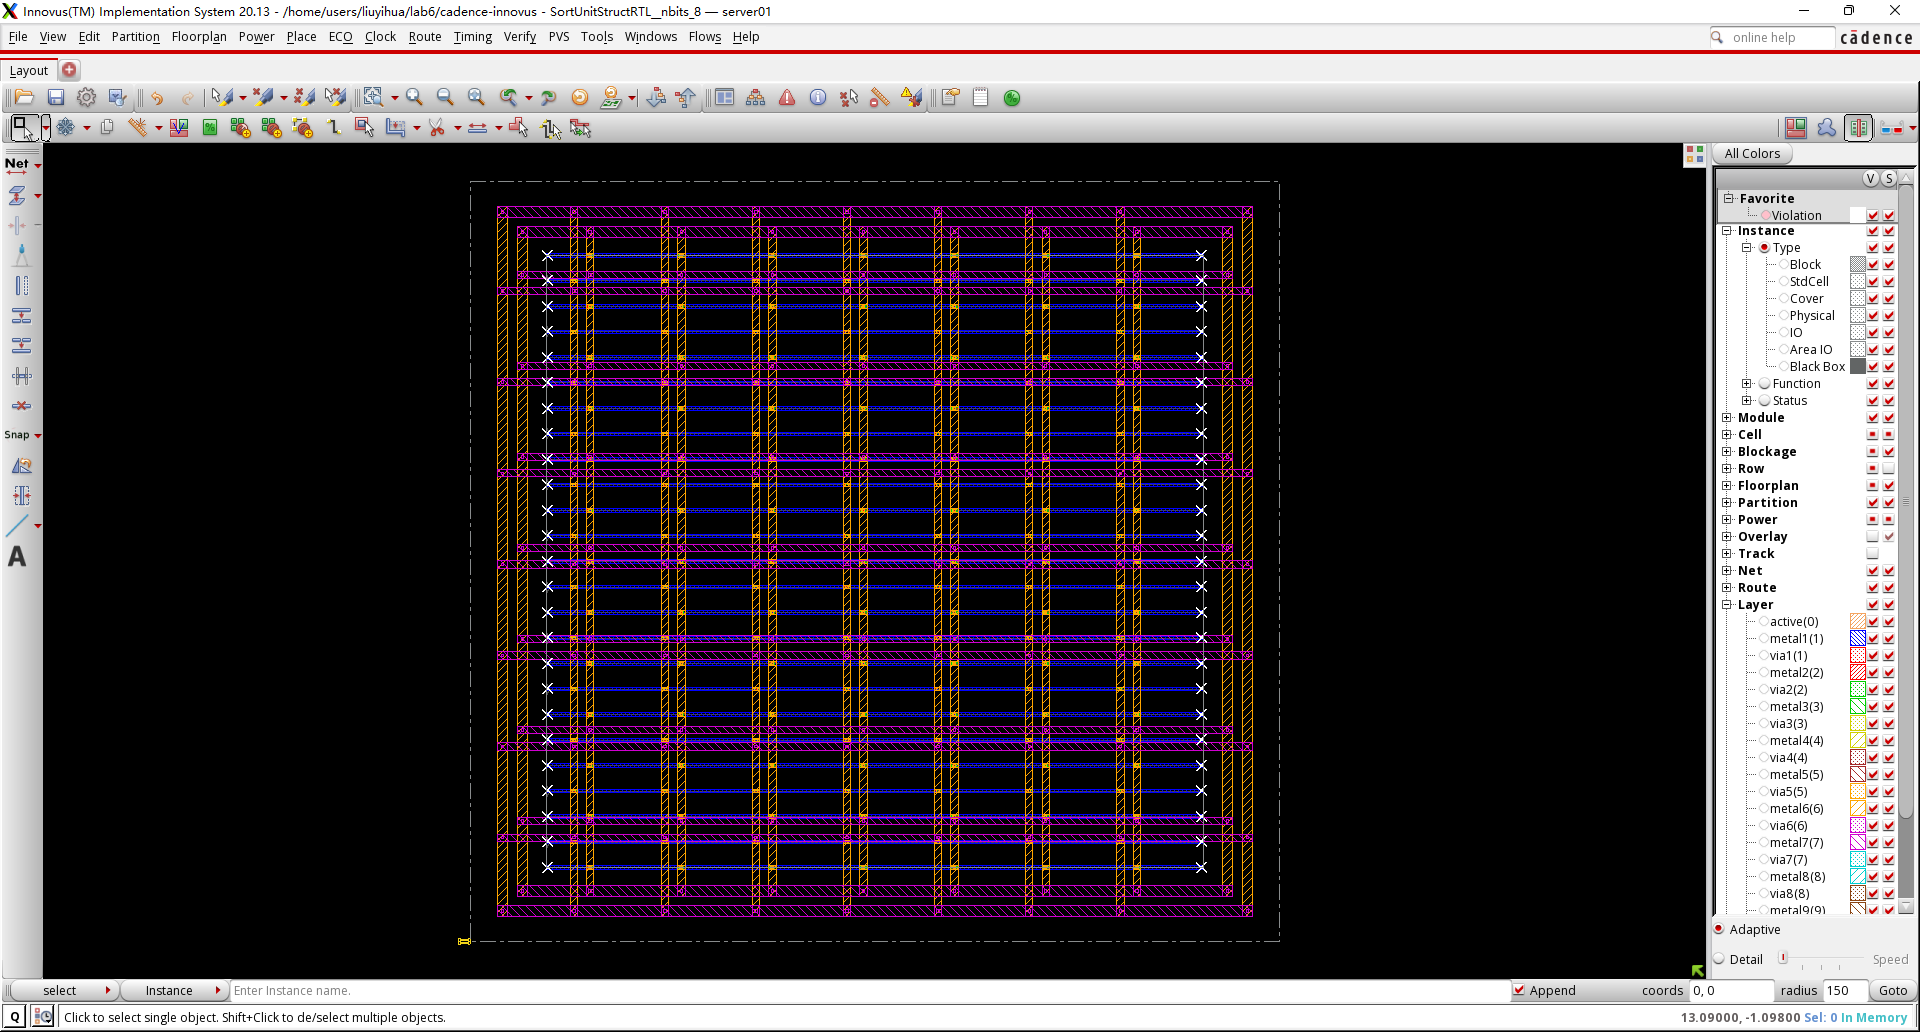
\includegraphics[width=\textwidth]{images/13.png}
\end{figure}
You can toggle the visibility of metal layers by using the panel on the right. Click the checkbox in the V column to toggle the visibility of the corresponding layer. You can also simply use the number keys on your keyboard. Pressing the 6 key will toggle M6, and pressing the 7 key will toggle M7. Zoom in on a via and toggle the visibility of the metal layers to see how Cadence Innovus has automatically inserted a via stack that goes from M1 all the way up to M6 or M7.

Now that we have finished our basic power planning, we can do the initial placement and routing of the standard cells using the \texttt{place\_design} command:
\begin{minted}{text}
innovus> place_design
\end{minted}
The following screen capture illustrates what you should see: the gates have been placed underneath a sea of wiring on the various metal layers.
\begin{figure}[H]
    \centering
    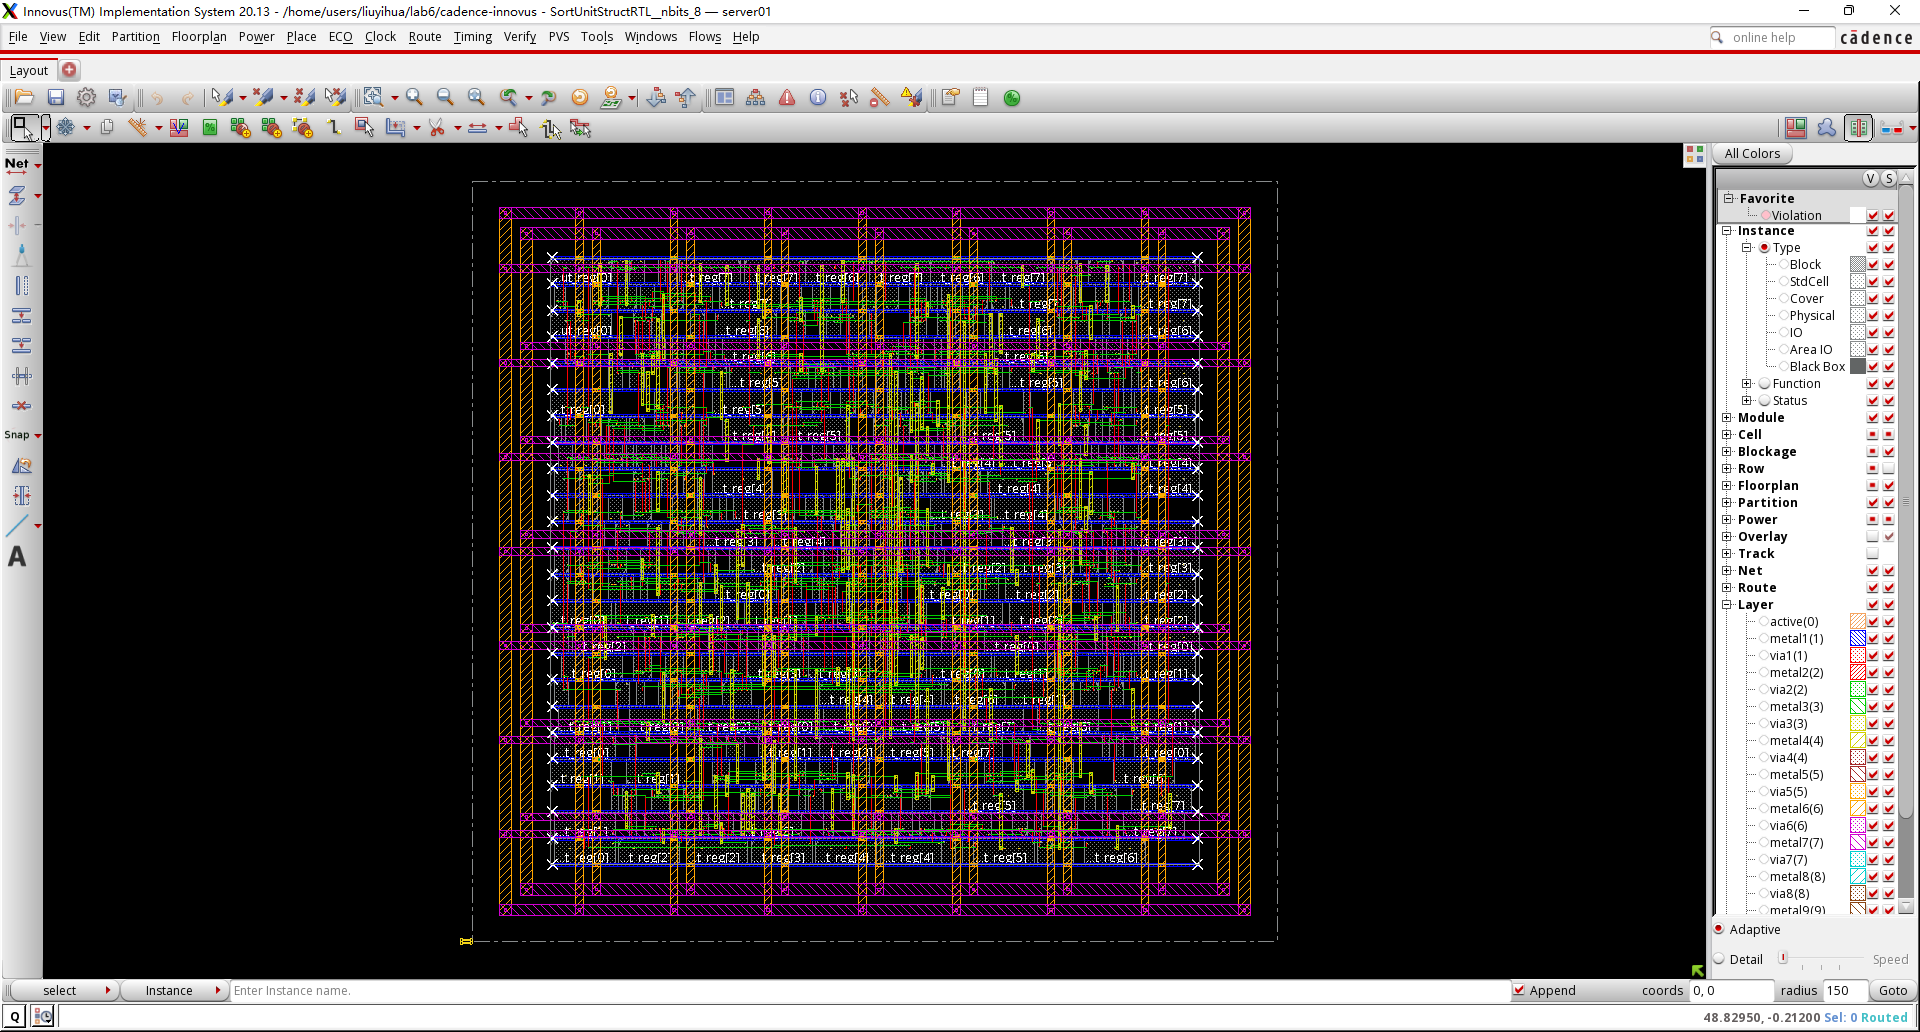
\includegraphics[width=\textwidth]{images/14.png}
\end{figure}
Note that Cadence Innovus has only done a very preliminary routing, primarily to help improve placement. You can use the Amobea workspace to help visualize how modules are mapped across the chip. Choose \textit{Windows > Workspaces > Amoeba} from the menu. However, we recommend using the design browser to help visualize how modules are mapped across the chip. Here are the steps:
\begin{itemize}
    \item Choose \textit{Windows > Workspaces > Design Browser + Physical} from the menu
    \item Hide all of the metal layers by pressing the number keys
    \item Browse the design hierarchy using the panel on the left
    \item Right click on a module, click \textit{Highlight}, select a color
\end{itemize}
In this way you can view where various modules are located on the chip. The following screen capture illustrates the location of the five \texttt{MinMaxUnit} modules.
\begin{figure}[H]
    \centering
    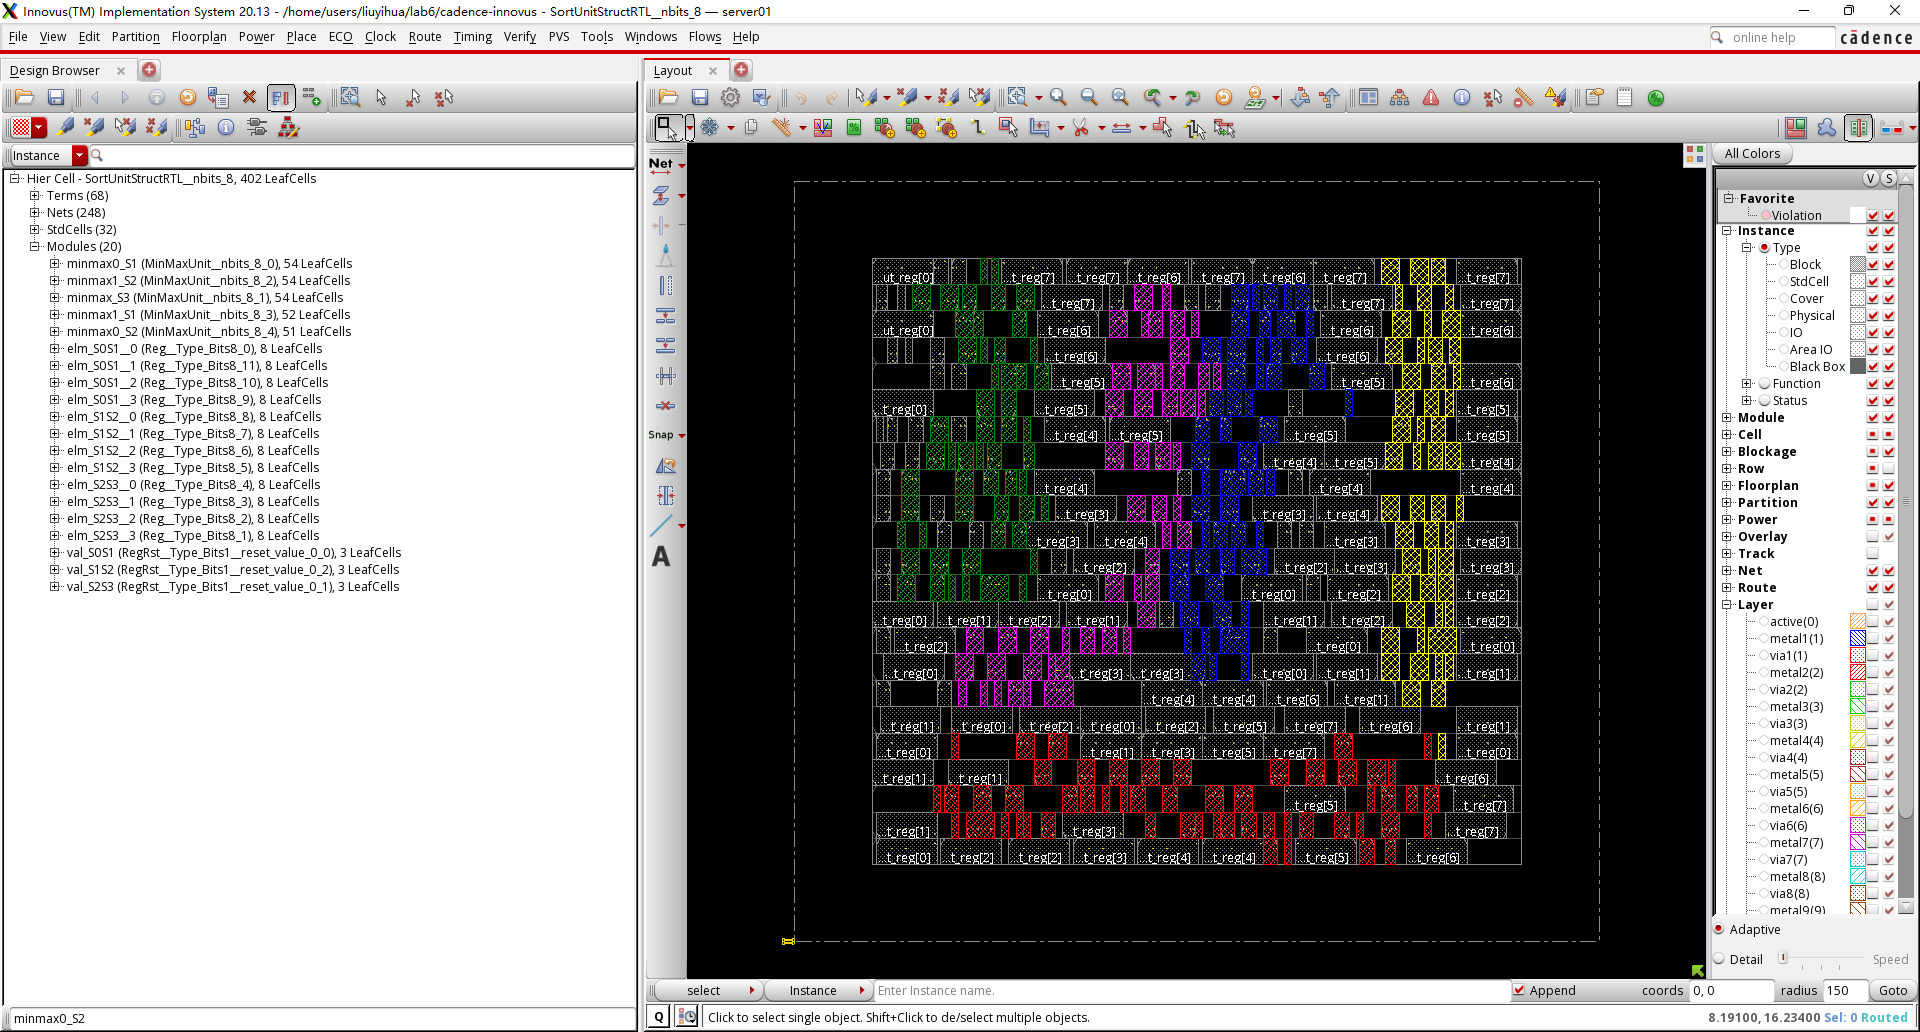
\includegraphics[width=\textwidth]{images/15.png}
\end{figure}
Notice how Cadence Innovus has grouped each module together. The placement algorithm tries to keep connected standard cells close together to minimize wiring.

The next step is to assign the IO pin location for our block-level design. Since this is not a full chip with IOcells, or a hierarchical block, we don’t really care exactly where all of the pins line up, so we’ll let the tool assign the location for all of the pins.
\begin{minted}{text}
innovus> assignIoPins -pin *
\end{minted}
The next step is to improve the quality of the clock tree routing. First, let’s display just the clock tree so we can clearly see the impact of optimized clock tree routing. In the right panel, click on Net and then deselect the checkbox in the V column next to Signal, Special Net, Power, and Ground so that only Clock is selected. You should be able to see the clock snaking around the chip connecting the clock port of all of the registers. Now use the \texttt{ccopt\_design} command to optimize the clock tree routing.
\begin{minted}{text}
innovus> ccopt_design
\end{minted}
If you watch closely, you should see a significant difference in the clock tree routing before and after optimization. The following screen capture illustrates the optimized clock tree routing.
\begin{figure}[H]
    \centering
    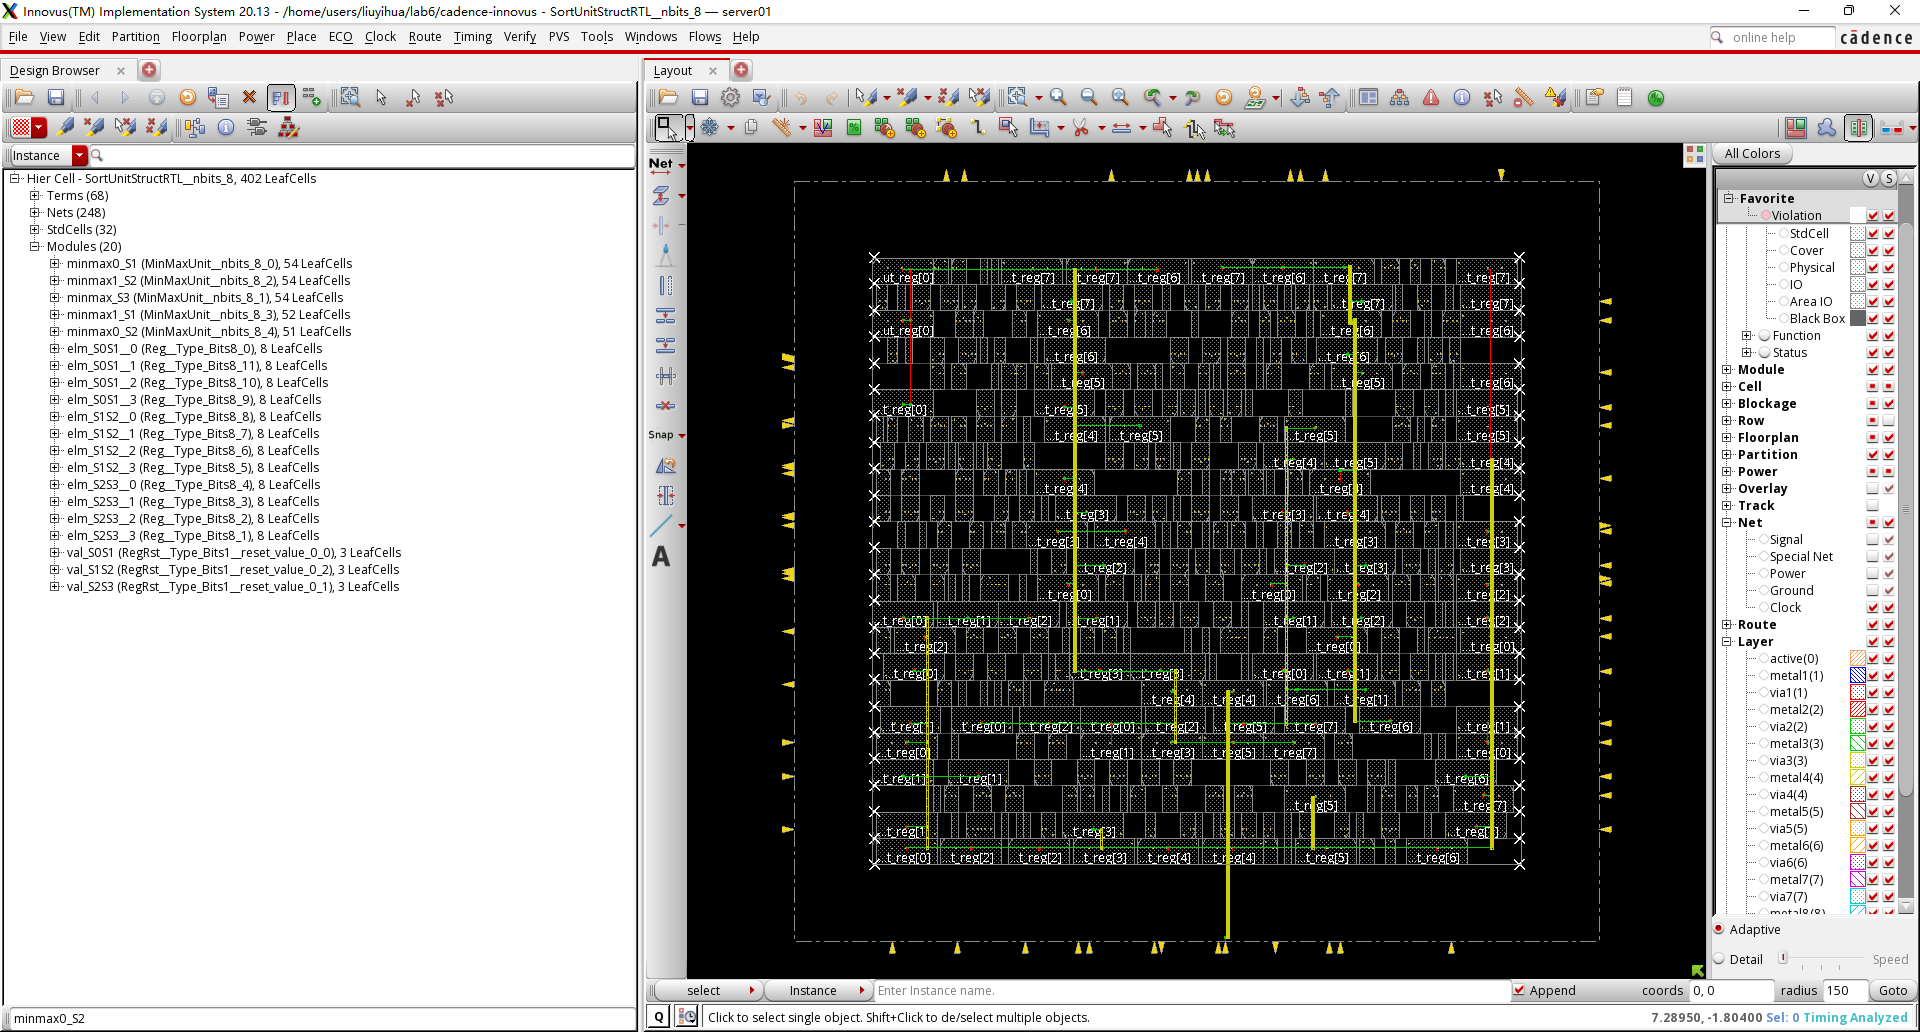
\includegraphics[width=\textwidth]{images/16.png}
\end{figure}
The routes are straighter, shorter, and well-balanced. This will result in a much lower clock skew.

To avoid hold time violations (situations where the contamination delay is smaller than the hold time and new data arrives too quickly), we include the following commands:
\begin{minted}[breaklines]{tcl}
setOptMode -holdFixingCells {BUF_X1}
setOptMode -holdTargetSlack 0.013 -setupTargetSlack 0.044;
optDesign -postCTS -outDir timingReports -prefix postCTS_hold -hold
\end{minted}
Here, we specified a list of buffer cells to the tool from \texttt{stdcells.v} that Innovus can use to add delays to paths that violate the hold time constraint. We then tell Innovus our hold and setup time constraints, in nanoseconds, these numbers were derived from the .lib file. Then, we actually fix any violating paths using the \texttt{optDesign} command.

If you look into the output of \texttt{optDesign}, you should see the following section:
\begin{minted}[breaklines]{text}
*** Finished Core Fixing (fixHold) cpu=0:00:01.0 real=0:00:01.0 totSessionCpu=0:01:45 mem=1638.9M density=71.439% ***

*info:
*info: Added a total of 56 cells to fix/reduce hold violation
*info:
*info: Summary:
*info:           56 cells of type 'BUF_X1' used
\end{minted}
This means that as a result of our hold time optimization, we have added 51 buffer cells to the netlist.

The next step is to improve the quality of the signal routing. Display just the signals but not the power and ground routing by clicking on the checkbox in the V column next to Signal in the left panel. Then use the \texttt{routeDesign} command to optimize the signal routing. We follow this with another iteration of \texttt{optDesign} to fix any violating paths that were created during \texttt{routeDesign}.
\begin{minted}[breaklines]{tcl}
routeDesign
optDesign -postRoute -outDir timingReports -prefix postRoute_hold -hold
\end{minted}
If you watch closely, you should see a significant difference in the signal routing before and after optimization. The following screen capture illustrates the optimized signal routing.
\begin{figure}[H]
    \centering
    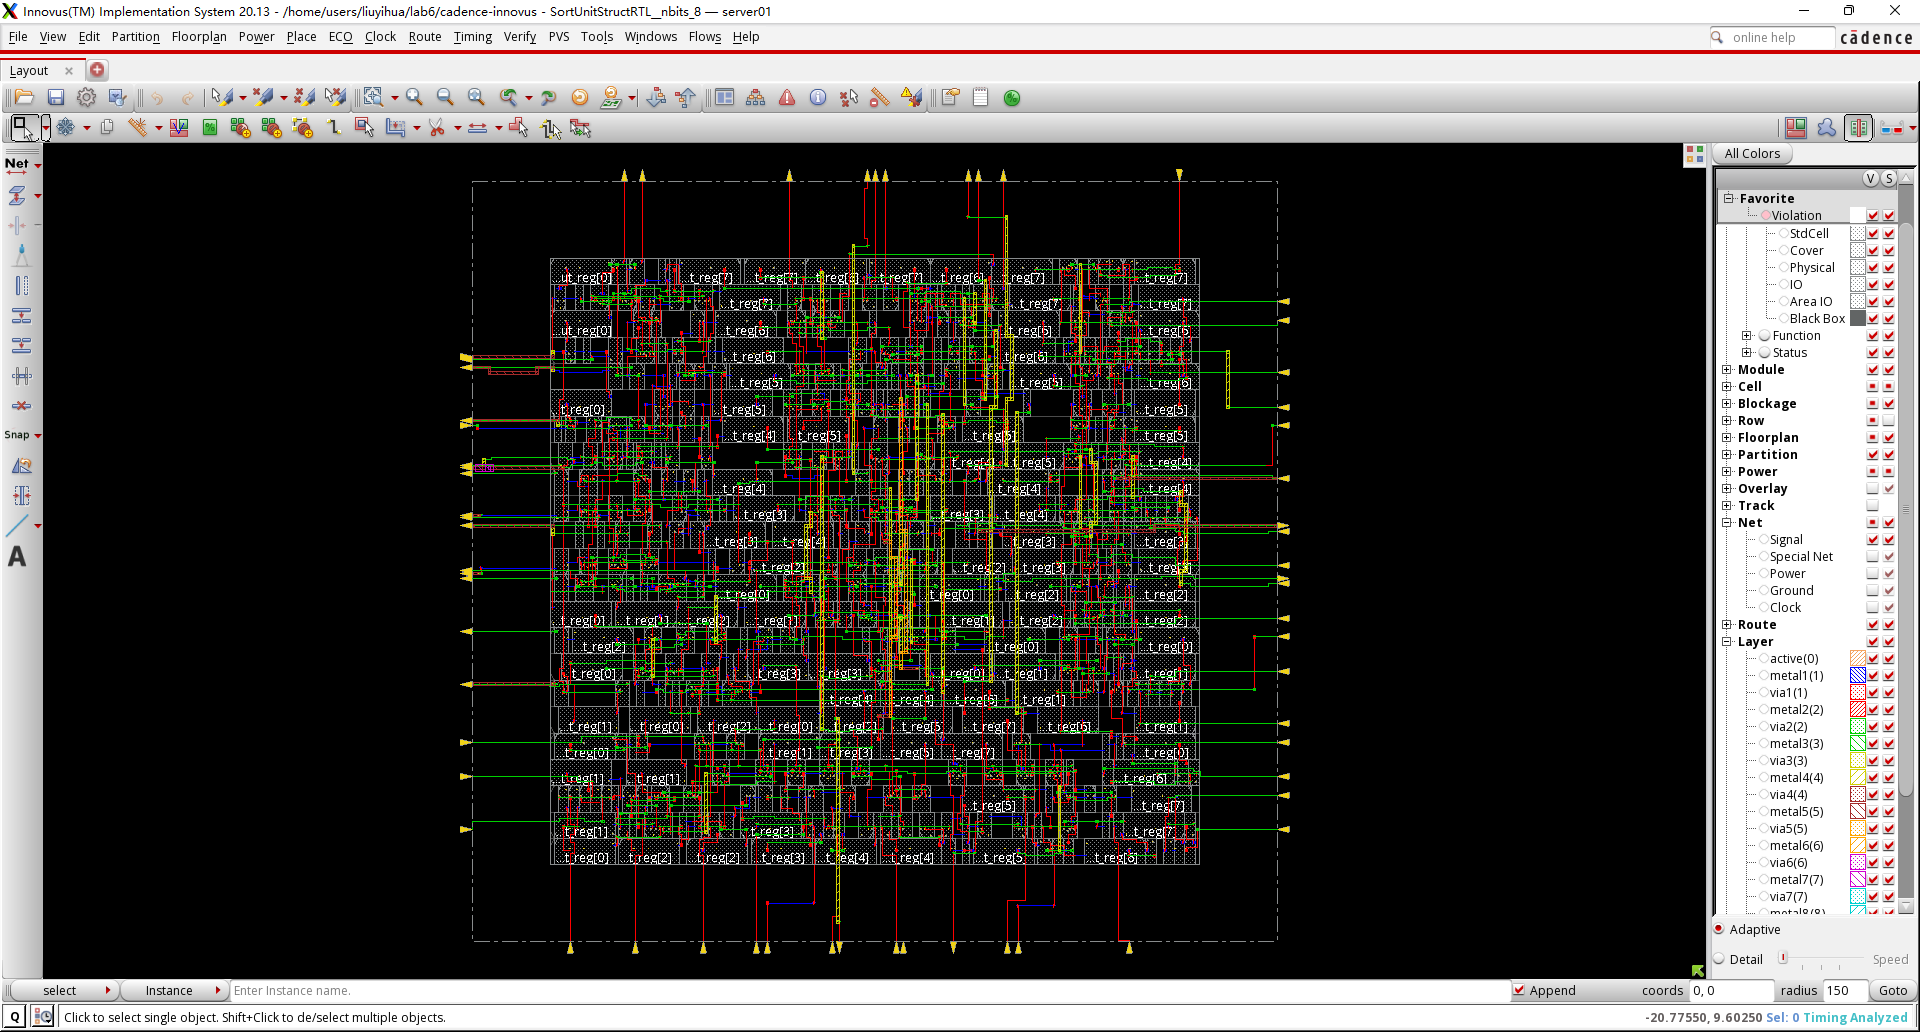
\includegraphics[width=\textwidth]{images/17.png}
\end{figure}
Again the routes are straighter and shorter. This will reduce the interconnect resistance and capacitance and thus improve the delay and energy of our design.

The final step is to insert “filler” cells. Filler cells are essentially empty standard cells whose sole purpose is to connect the wells across each standard cell row.
\begin{minted}[breaklines]{tcl}
setFillerMode -corePrefix FILL -core "FILLCELL_X4 FILLCELL_X2 FILLCELL_X1"
addFiller
\end{minted}
Zoom in to see some of the detailed routing and take a moment to appreciate how much effort the tools have done for us automatically to synthesize, place, and route this design. The following screen capture shows some of this detailed routing.
\begin{figure}[H]
    \centering
    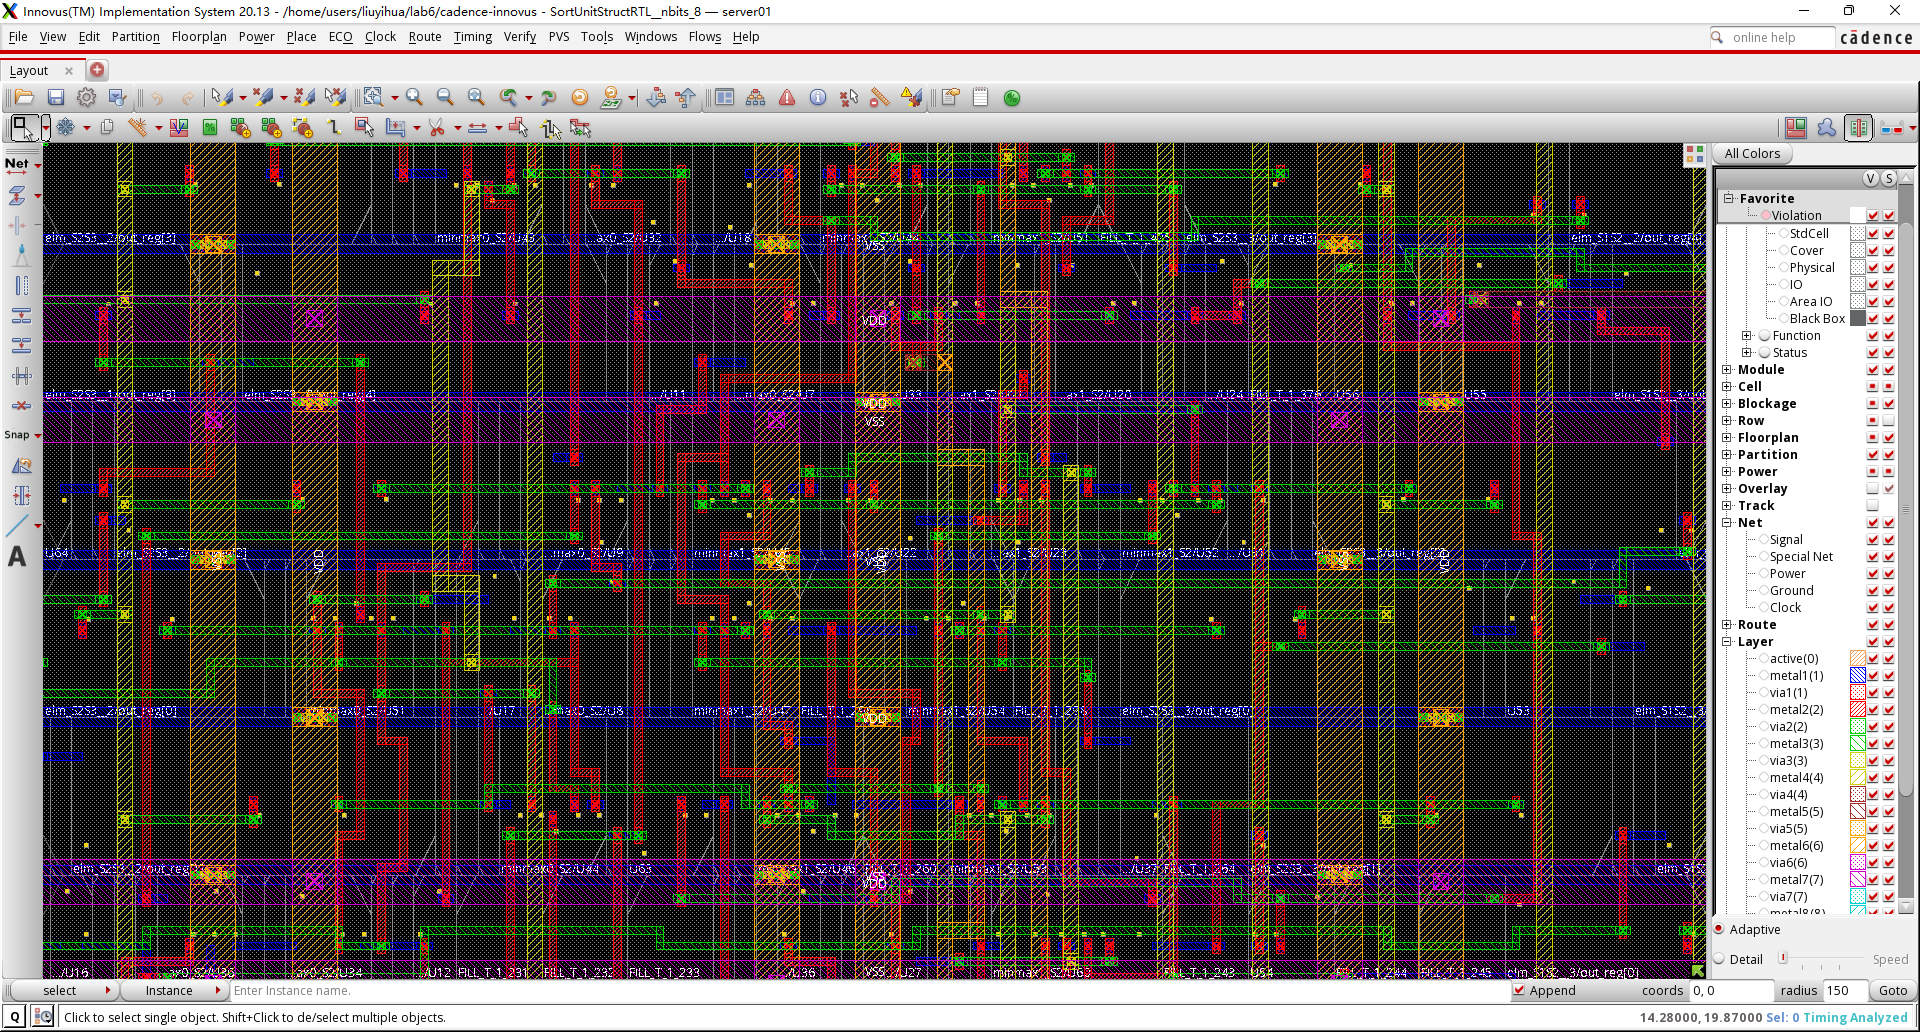
\includegraphics[width=\textwidth]{images/18.png}
\end{figure}
Notice how each metal layer always goes in the same direction. So M2 is always vertical, M3 is always horizontal, M4 is always vertical, etc. This helps reduce capacitive coupling across layers and also simplifies the routing algorithm. Actually, if you look closely at the above screen shot, you can see situations on M2 (red) and M3 (green) where the router has generated a little “jog” meaning that on a single layer, the wire goes both vertically and horizontally. This is an example of the sophisticated algorithms used in these tools.

Our design is now on silicon! Obviously, there are many more steps required before you can really tape out a chip. We would need to add an I/O ring with pads so we can connect the chip to the package, we would need to do further verification and additional optimization.

For example, one thing we want to do is verify that the gate-level netlist matches what is really in the final layout. We can do this using the \texttt{verifyConnectivity} command. We can also do a preliminary “design rule check” to make sure that the generated metal interconnect does not violate any design rules with the \texttt{verify\_drc} command.
\begin{minted}[breaklines]{tcl}
verifyConnectivity
verify_drc
\end{minted}
Now we can generate various output files. We might want to save the final gate-level netlist for the chip since Cadence Innovus will often insert new cells or change cells during its optimization passes.
\begin{minted}{text}
innovus> saveNetlist post-par.v
\end{minted}
We can also extract resistance and capacitance for the metal interconnect and write this to a special .spef file. This file can be used for later timing and/or power analysis.
\begin{minted}[breaklines]{tcl}
extractRC
rcOut -rc_corner typical -spef post-par.spef
\end{minted}
You may get an error regarding open nets. This is actually more of a warning message, and for the purposes of RC extraction we can ignore this.

We also need to extract delay information and write this to a .sdf (Standard Delay Format) file, which we’ll use for our back-annotated gate-level simulations.
\begin{minted}{text}
innovus> write_sdf post-par.sdf -interconn all -setuphold split
\end{minted}
Finally, we, of course, need to generate the real layout as a .gds file. This is what we will send to the foundry when we are ready to tapeout the chip.
\begin{minted}[breaklines]{text}
innovus> streamOut post-par.gds -merge "$env(ECE4810J_STDCELLS)/stdcells.gds" -mapFile "$env(ECE4810J_STDCELLS)/rtk-stream-out.map"
\end{minted}
We can also use Cadence Innovus to do timing, area, and power analysis, similar to what we did with Synopsys DC. These post-place-and-route results will be much more accurate than the preliminary post-synthesis results. Let’s start with a basic timing report.
\begin{minted}[breaklines,breakanywhere]{text}
innovus> report_timing
...
Other End Arrival Time         -0.000
- Setup                         0.044
+ Phase Shift                   0.600
+ CPPR Adjustment               0.000
= Required Time                 0.556
- Arrival Time                  0.485
= Slack Time                    0.071
     Clock Rise Edge                 0.000
     + Clock Network Latency (Prop)  -0.000
     = Beginpoint Arrival Time       -0.000
     +-----------------------------------------------------------------------------------------------+
     |               Instance                |     Arc      |   Cell    | Delay | Arrival | Required |
     |                                       |              |           |       |  Time   |   Time   |
     |---------------------------------------+--------------+-----------+-------+---------+----------|
     | elm_S1S2__2/out_reg[1]                | CK ^         |           |       |  -0.000 |    0.071 |
     | elm_S1S2__2/out_reg[1]                | CK ^ -> Q v  | DFF_X1    | 0.085 |   0.085 |    0.155 |
     | minmax0_S2/FE_DBTC7_elm_S1S2__out_2_1 | A v -> ZN ^  | INV_X1    | 0.021 |   0.106 |    0.177 |
     | minmax0_S2/U57                        | B1 ^ -> ZN v | AOI21_X1  | 0.016 |   0.122 |    0.192 |
     | minmax0_S2/U58                        | B1 v -> ZN ^ | AOI222_X1 | 0.078 |   0.200 |    0.270 |
     | minmax0_S2/U36                        | A1 ^ -> ZN v | NOR3_X1   | 0.013 |   0.213 |    0.284 |
     | minmax0_S2/U9                         | A1 v -> ZN ^ | NOR3_X1   | 0.039 |   0.252 |    0.323 |
     | minmax0_S2/U33                        | A1 ^ -> ZN v | NOR3_X1   | 0.012 |   0.265 |    0.335 |
     | minmax0_S2/U28                        | A1 v -> ZN ^ | NOR3_X1   | 0.035 |   0.300 |    0.370 |
     | minmax0_S2/U59                        | A1 ^ -> ZN v | OAI22_X1  | 0.022 |   0.322 |    0.393 |
     | minmax0_S2/U5                         | A v -> ZN ^  | OAI21_X1  | 0.024 |   0.346 |    0.417 |
     | minmax0_S2/FE_OFC0_n7                 | A ^ -> Z ^   | CLKBUF_X1 | 0.106 |   0.452 |    0.523 |
     | minmax0_S2/U46                        | B1 ^ -> ZN v | OAI22_X1  | 0.033 |   0.485 |    0.555 |
     | elm_S2S3__0/out_reg[1]                | D v          | DFF_X1    | 0.000 |   0.485 |    0.556 |
     +-----------------------------------------------------------------------------------------------+
\end{minted}
Note that for these results we used a target clock period of 0.6ns. This was the shortest clock period which still met timing without any negative slack during synthesis. From the above report, we can see that our design is still meeting timing even after place-and-route. Note that it is very likely that the critical path identified by Synopsys DC after synthesis will \textit{not} be the same critical path identified by Cadence Innovus after place-and-route. This is because Synopsys DC can only guess the final placement of the cells and interconnect during static timing analysis, while Cadence Innovus can use the real placement of the cells and interconnect during static timing analysis. For the same reason, there is no guarantee that if your design meets timing after synthesis that it will still meet timing after place-and-route! It is very possible that your design \textit{will} meet timing after synthesis, and then \textit{will not} meet timing after place-and-route. If your design does not meet timing after place-and-route, you must go back and use a longer target clock period for synthesis!

You can use the following steps in Cadence Innovus to display where the critical path is on the actual chip.
\begin{itemize}
    \item Choose \textit{Timing > Debug Timing} from the menu
    \item Click \textit{OK} in the pop-up window
    \item Right-click on the first path in the \textit{Path List}
    \item Choose \textit{Highlight > Only This Path > Color}
\end{itemize}
You can also use the Design Browser to highlight specific modules to visualize how the critical path is routed across the chip between these modules. The following screen capture illustrates the critical path in our three-stage sort unit. From the above timing report, we know the critical path basically goes through the \texttt{minmax0\_S2} module, so we have highlighted that module in red using the Design Browser. Cadence Innovus has worked hard in both placement and routing to keep the critical path short. If your critical path stretches across the entire chip, you may need to take extra steps, such as explicit floorplanning or hierarchical design, to help the tools produce a better quality result.
\begin{figure}[H]
    \centering
    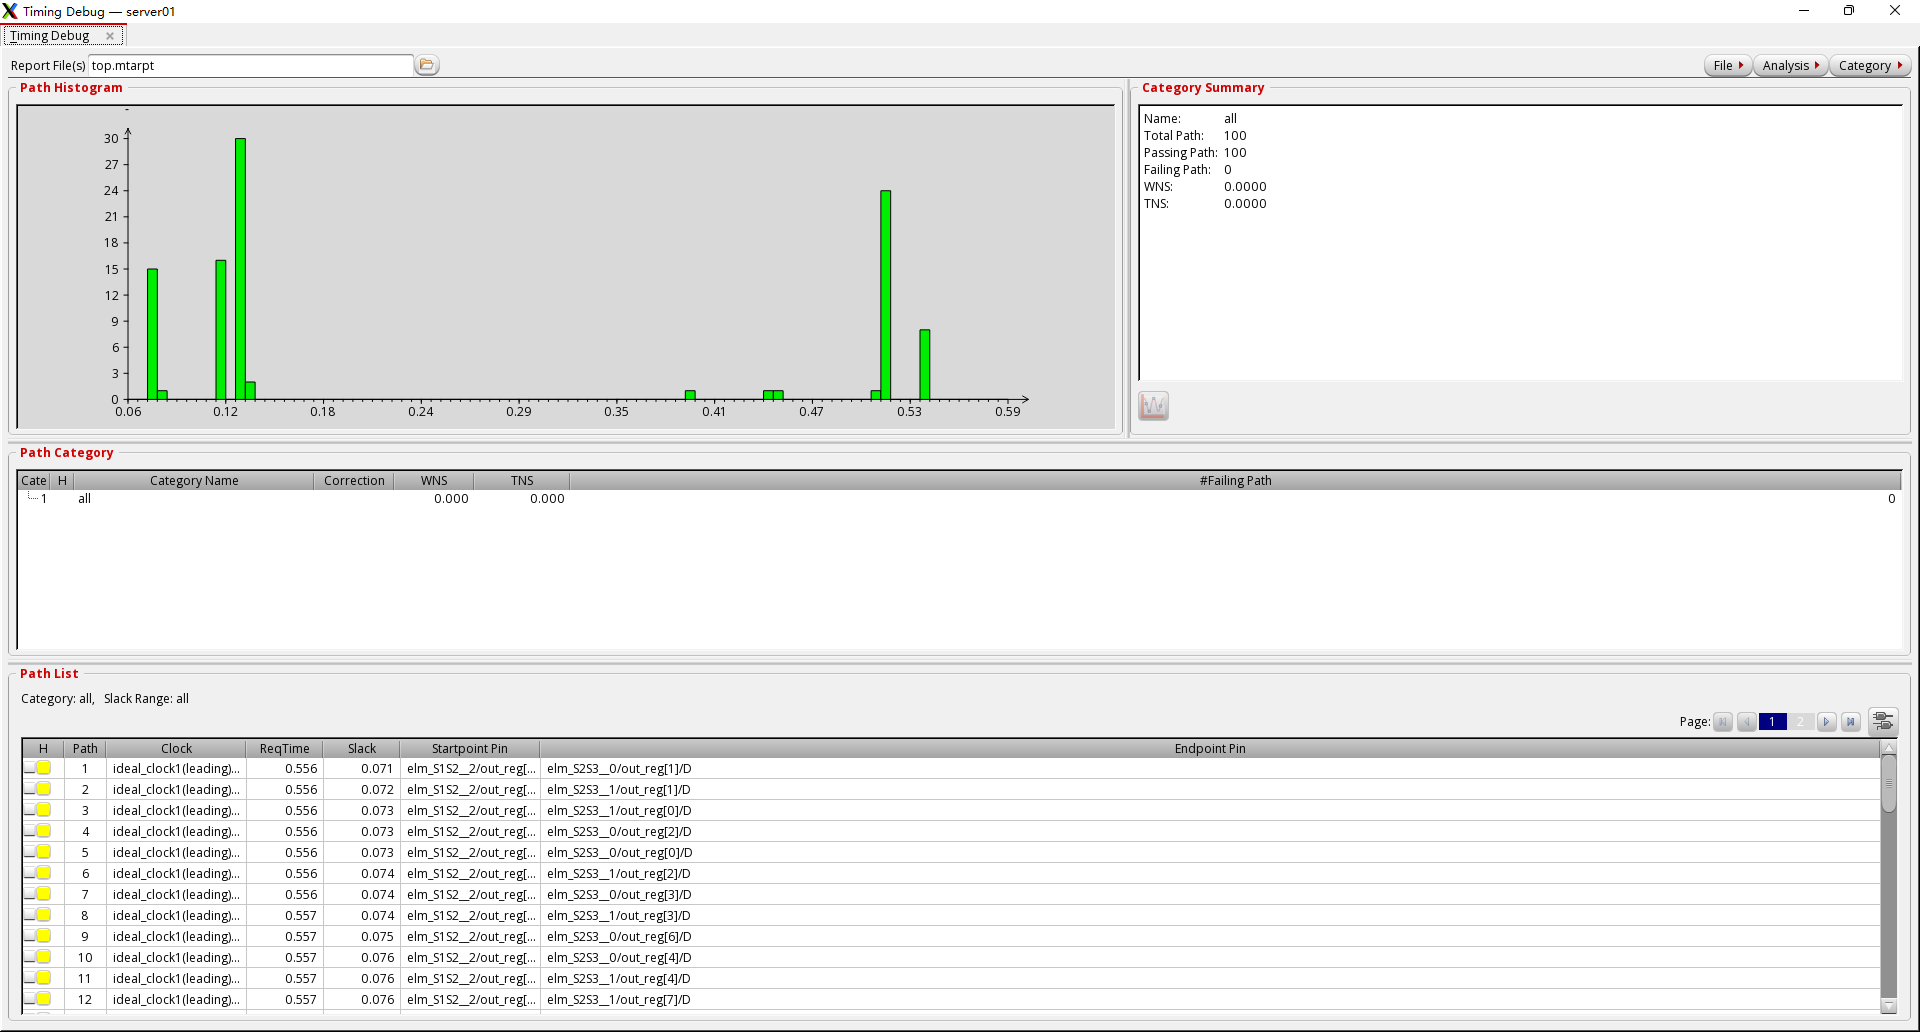
\includegraphics[width=\textwidth]{images/19.png}
\end{figure}
\begin{figure}[H]
    \centering
    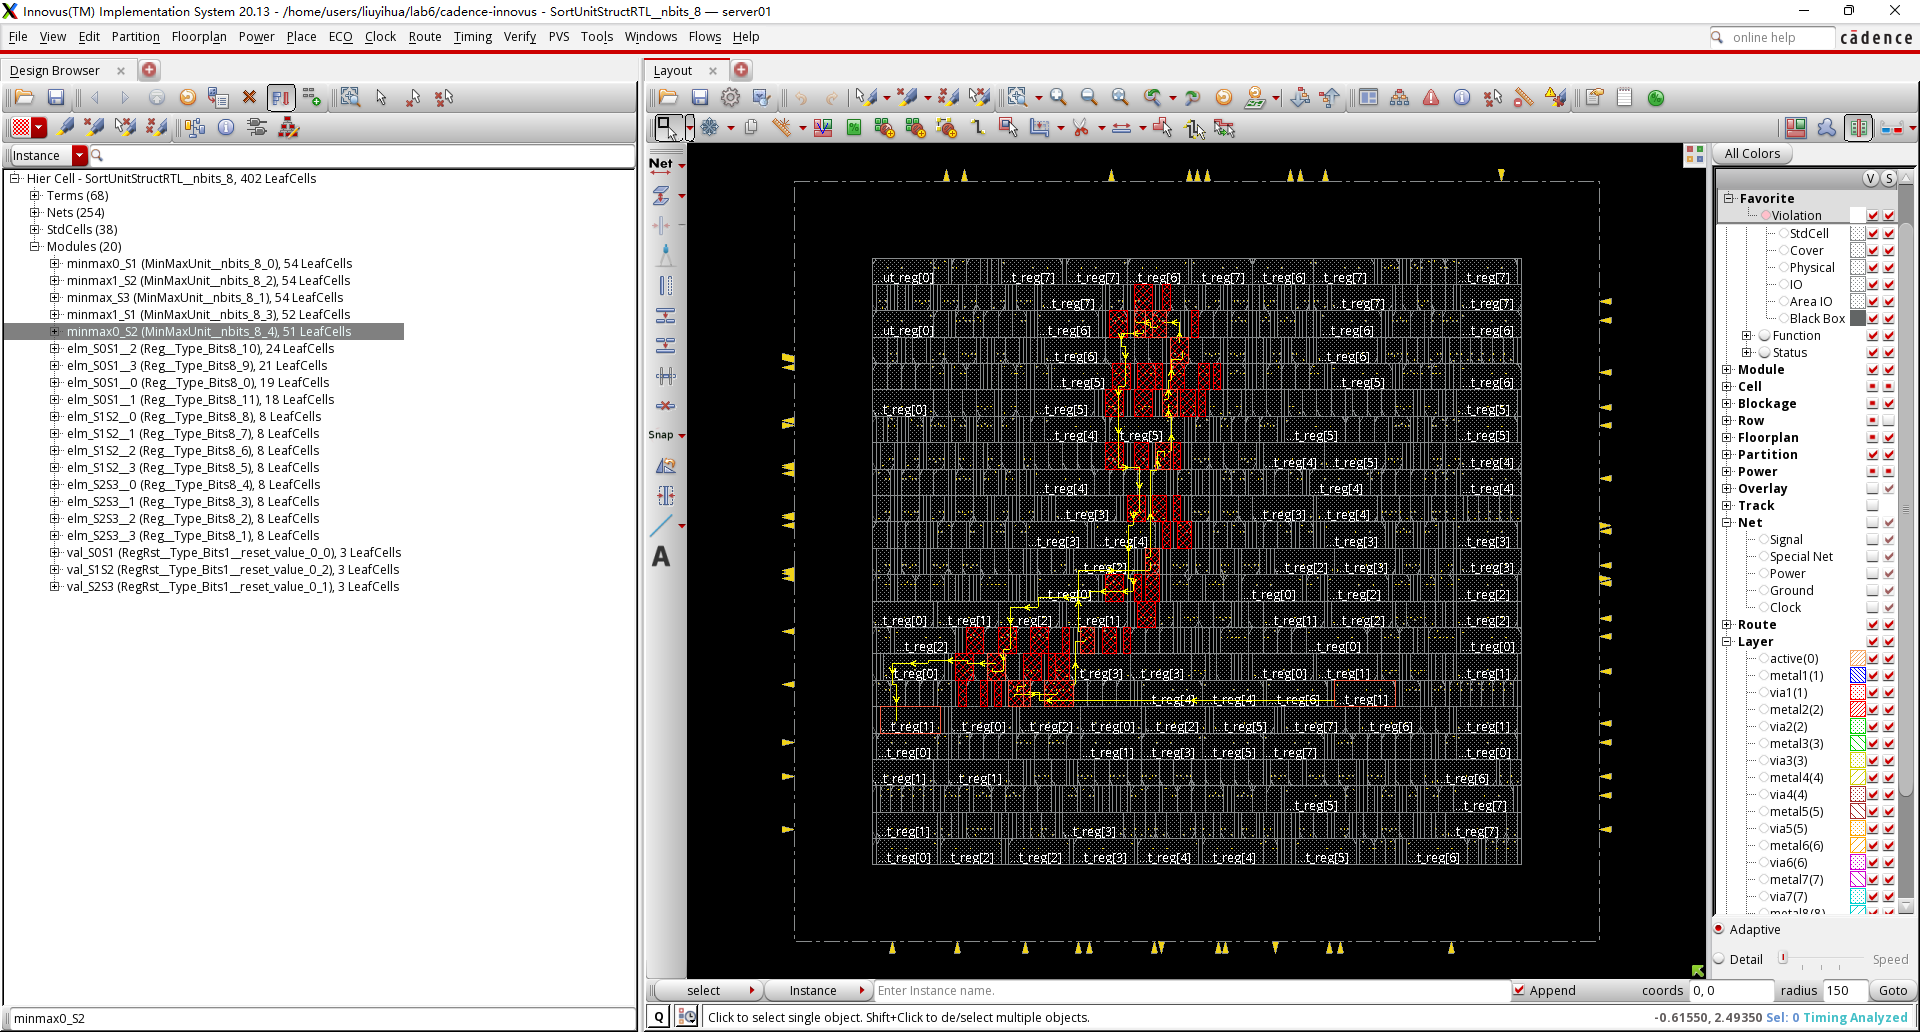
\includegraphics[width=\textwidth]{images/20.png}
\end{figure}
As in Synopsys DC, the \texttt{report\_area} command can show the area each module uses and can enable detailed area breakdown analysis. These area results will be far more accurate than the post-synthesis results.
\begin{minted}[breaklines,breakanywhere]{text}
innovus> report_area
    Hinst Name             Module Name                         Inst Count           Total Area
-------------------------------------------------------------------------------------------
SortUnitStructRTL__nbits_8                                            458              791.084
 elm_S0S1__0               Reg__Type_Bits8_0                           19               44.954
 elm_S0S1__1               Reg__Type_Bits8_11                          18               44.156
 elm_S0S1__2               Reg__Type_Bits8_10                          24               48.944
 elm_S0S1__3               Reg__Type_Bits8_9                           21               46.550
 elm_S1S2__0               Reg__Type_Bits8_8                            8               36.176
 elm_S1S2__1               Reg__Type_Bits8_7                            8               36.176
 elm_S1S2__2               Reg__Type_Bits8_6                            8               36.176
 elm_S1S2__3               Reg__Type_Bits8_5                            8               36.176
 elm_S2S3__0               Reg__Type_Bits8_4                            8               36.176
 elm_S2S3__1               Reg__Type_Bits8_3                            8               36.176
 elm_S2S3__2               Reg__Type_Bits8_2                            8               36.176
 elm_S2S3__3               Reg__Type_Bits8_1                            8               36.176
 minmax0_S1                MinMaxUnit__nbits_8_0                       54               52.934
 minmax0_S2                MinMaxUnit__nbits_8_4                       51               50.274
 minmax1_S1                MinMaxUnit__nbits_8_3                       52               51.338
 minmax1_S2                MinMaxUnit__nbits_8_2                       54               52.934
 minmax_S3                 MinMaxUnit__nbits_8_1                       54               53.200
 val_S0S1                  RegRst__Type_Bits1__reset_value_0_0          3                5.852
 val_S1S2                  RegRst__Type_Bits1__reset_value_0_2          3                5.852
 val_S2S3                  RegRst__Type_Bits1__reset_value_0_1          3                5.852
\end{minted}
The \texttt{\#Inst} column indicates the number of non-filler cells in that module. There are a total of 369 standard cells in the design. Each register has eight standard cells; eight flip-flops since it is an eight-bit register. The \texttt{MinMaxUnit}s have a different number of cells since they have been optimized differently. The \texttt{MinMaxUnit} consume about $\sim$40\% of the area.

As in Synopsys DC, the \texttt{report\_power} command can show how much power each module consumes. Note that this power analysis is still not that useful yet, since at this stage of the flow, the power analysis is still based purely on statistical activity factor estimation. We will do a more realistic power analysis in the next section.
\begin{minted}{text}
innovus> report_power -hierarchy all
\end{minted}
Finally, we go ahead and exit Cadence Innovus.
\begin{minted}{text}
innovus> exit
\end{minted}
We can now look at the actual \texttt{.gds} file for our design to see the final layout, including all of the cells and the interconnect using the open-source Klayout GDS viewer. Choose \textit{Display > Full Hierarchy} from the menu to display the entire design. Zoom in and out to see the individual transistors as well as the entire chip.
\begin{minted}{bash}
cd $TOPDIR/cadence-innovus
klayout -l $ECE4810J_STDCELLS/klayout.lyp post-par.gds
\end{minted}
The following screen capture illustrates using Klayout to view the layout for the entire sort unit.
\begin{figure}[H]
    \centering
    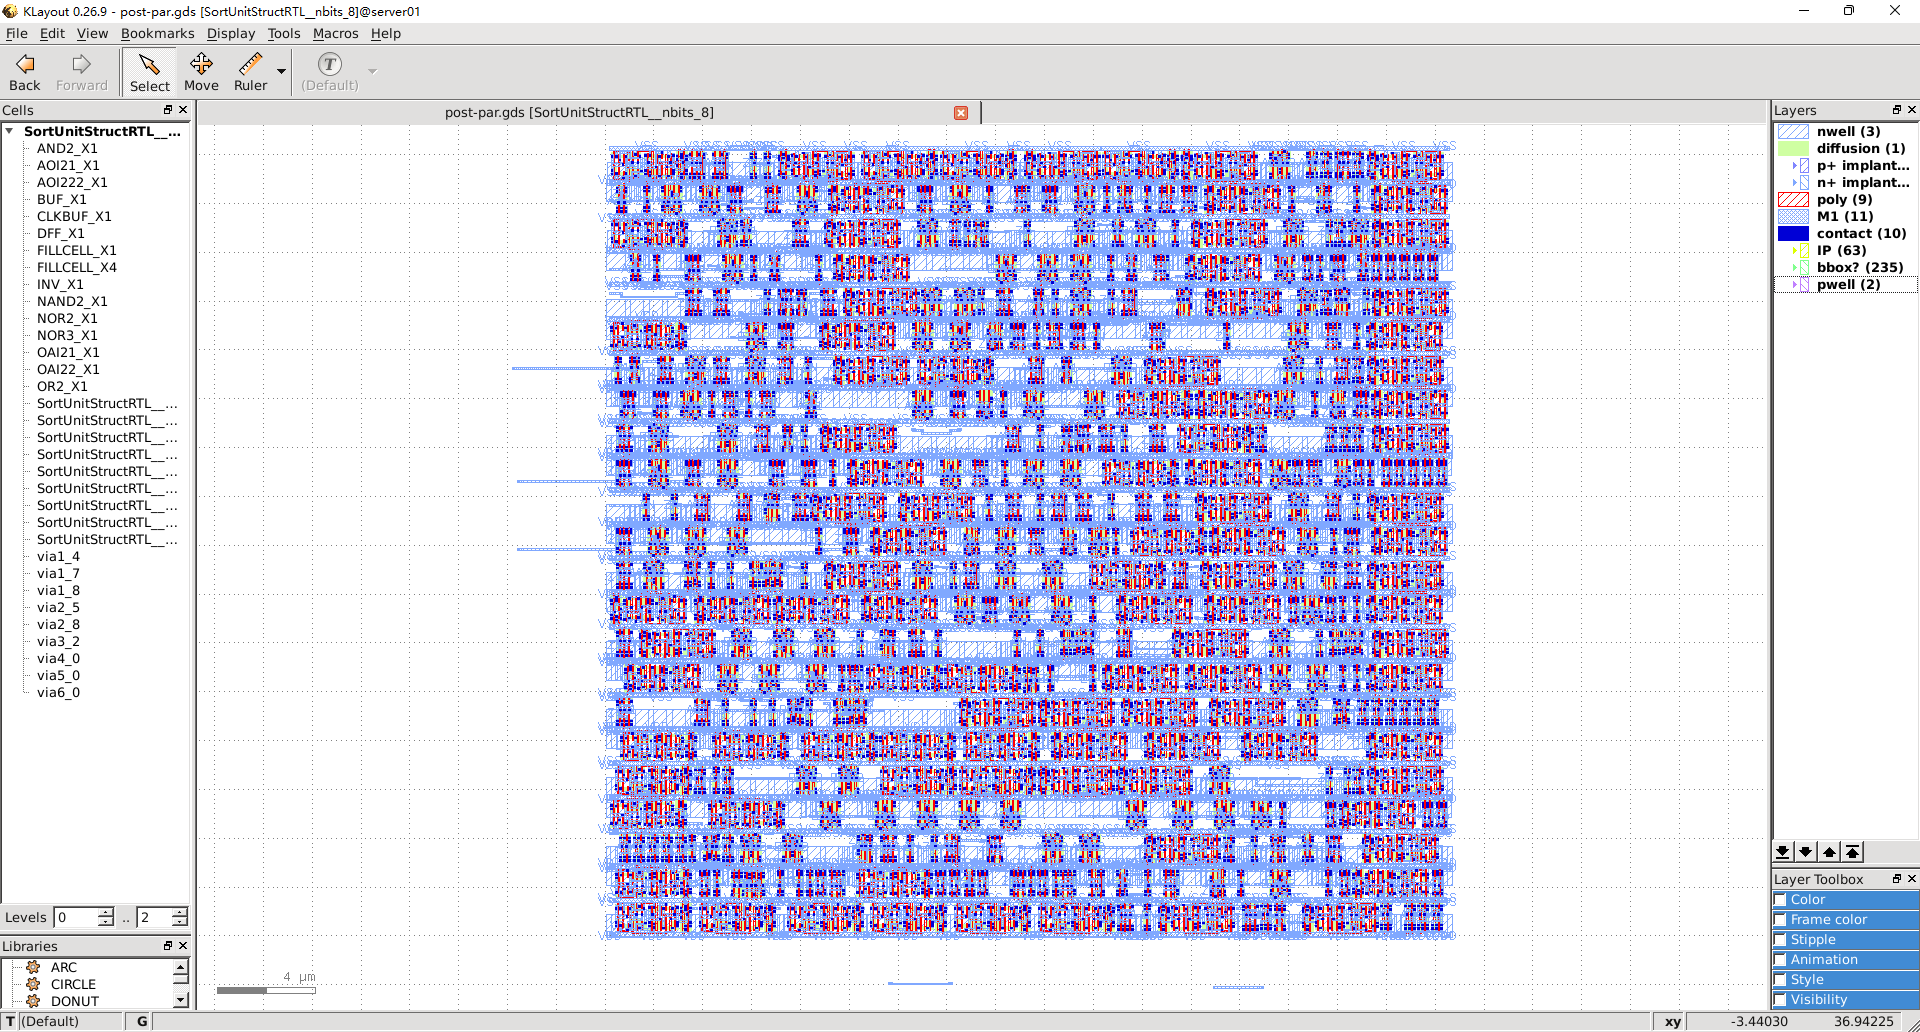
\includegraphics[width=\textwidth]{images/21.png}
\end{figure}
The following figure shows a zoomed portion of the layout. You can clearly see the active layer inside the standard cells, along with the signal routing on the lower metal layers. The power routing on the upper metal layers has been hidden for clarity.
\begin{figure}[H]
    \centering
    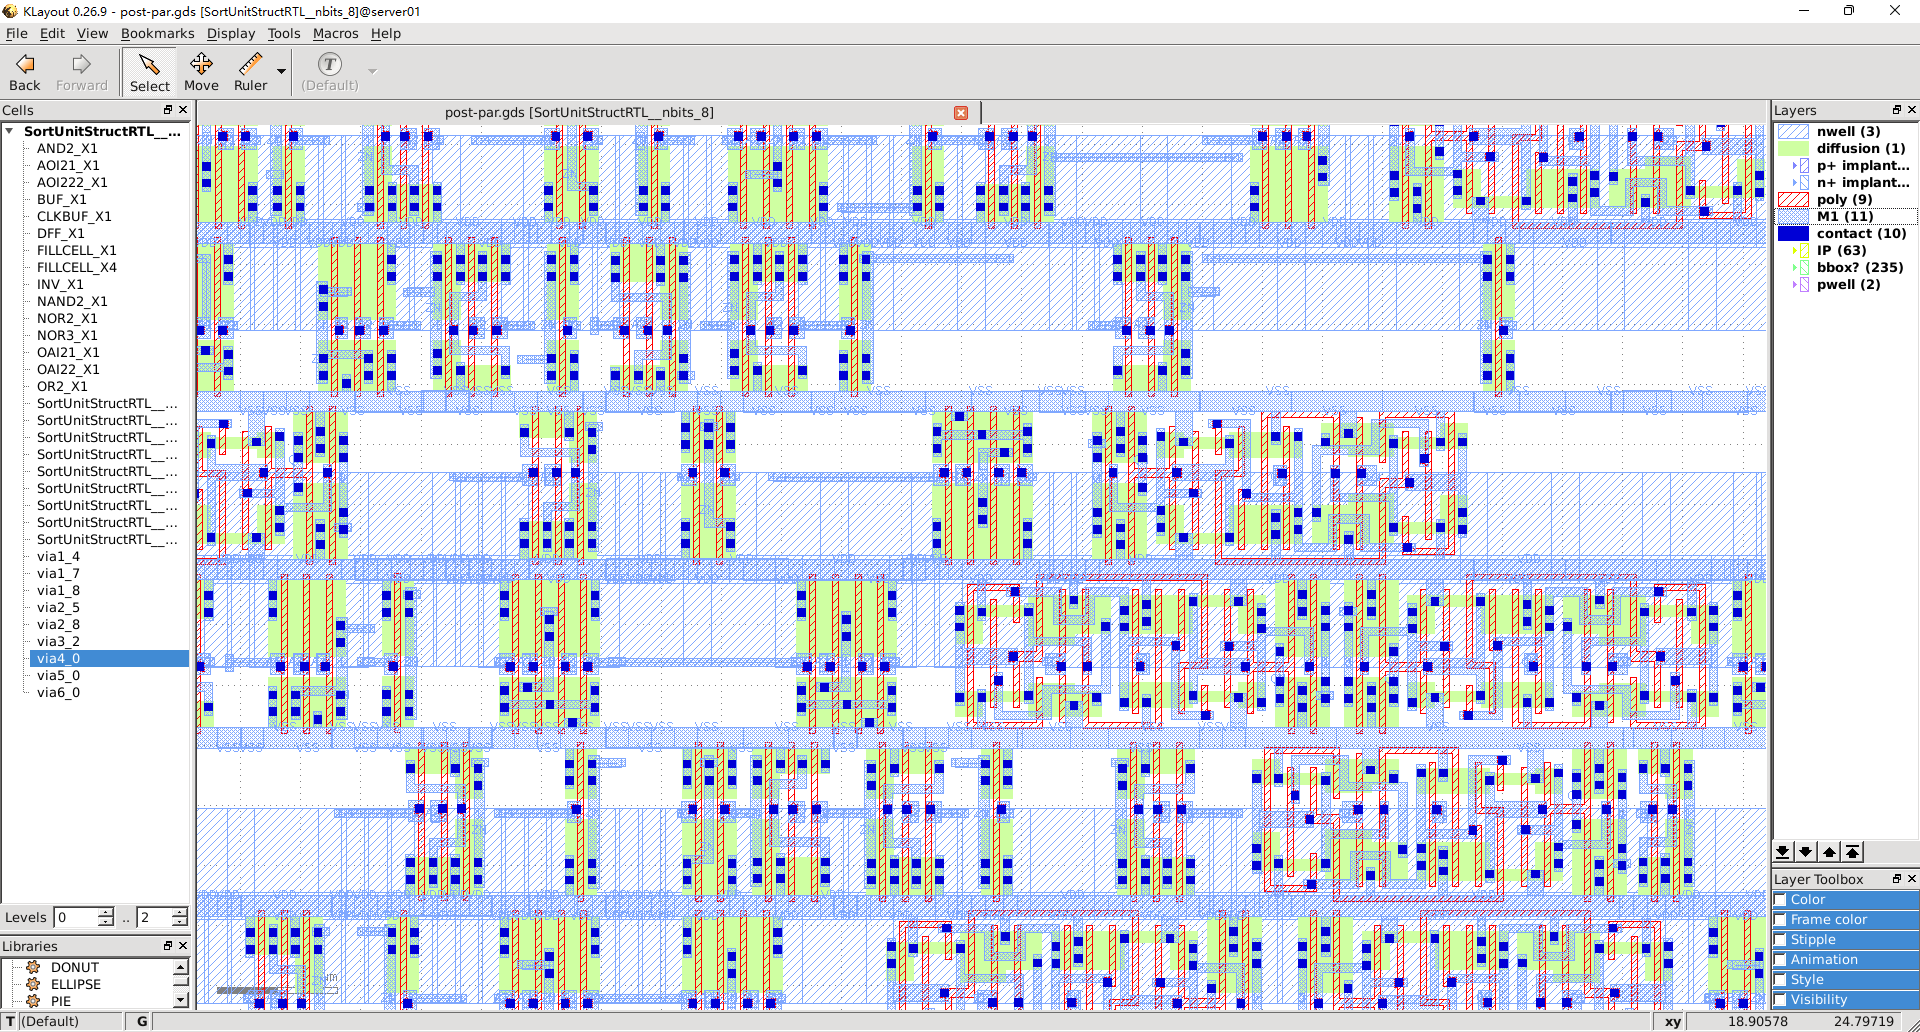
\includegraphics[width=\textwidth]{images/22.png}
\end{figure}
\subsection{Using Synopsys VCS for Back-Annotated Gate-Level Simulation}
Before place and route, we used Synopsys VCS to do a 4-state simulation and gate-level simulation. This time, we’ll be using VCS to perform a back-annotated gate-level simulation. The key difference between the previous gate-level simulation and this one is that in this case, we’ll be using a .sdf file to annotate delays in the gate-level simulation. In previous simulations, we only see signals change on the clock edge; however, with a back-annotated simulation, we’ll know more precisely when signals are arriving by using the delay information provided by the .sdf. This means that running a back-annotated simulation with a cycle time that is too fast will cause the design to fail! Back-annotated simulations are also useful for detecting hold-time violations.

Given the more realistic timing implications of a back-annotated simulation, we need to be more careful about the cycle time, input delay, and output delay that we provide to VCS. We’ll start by creating a build directory for our post-synth run of VCS, and output directories for the .vcd and .saif that we’ll generate for power analysis.
\begin{minted}{bash}
mkdir -p $TOPDIR/vcs-postpnr-build
cd $TOPDIR/vcs-postpnr-build
\end{minted}
Then we’ll run \texttt{vcs} and \texttt{./simv} to run our gate-level simulation on the sort-rtl-struct-random simulator testbench. Notice the differences between this command and the fast functional gate-level simulation command:
\begin{minted}[breaklines,breakanywhere]{bash}
vcs ../cadence-innovus/post-par.v $ECE4810J_STDCELLS/stdcells.v -full64 -sverilog +incdir+../sim/build +lint=all -xprop=tmerge -top SortUnitStructRTL__nbits_8_tb ../sim/build/SortUnitStructRTL__nbits_8_sort-rtl-struct-random_tb.v +sdfverbose -sdf min:SortUnitStructRTL__nbits_8_tb.DUT:../cadence-innovus/post-par.sdf +define+CYCLE_TIME=0.6 +define+VTB_INPUT_DELAY=0.03 +define+VTB_OUTPUT_ASSERT_DELAY=0.57 +vcs+dumpvars+SortUnitStructRTL__nbits_8_sort-rtl-struct-random_vcs.vcd +neg_tchk -override_timescale=1ns/1ps
./simv
\end{minted}
This time, we add the flag \texttt{+neg\_tchk}, which enables negative values in timing checks. Negative values in timing checks are important for cells that have negative hold times, for example. We also include the \texttt{+sdfverbose} flag, which reads in the \texttt{post-par.sdf}. Note that we also assign non-zero values for \texttt{+define+VTB\_INPUT\_DELAY} and \texttt{+define+VTB\_\\
OUTPUT\_ASSERT\_DELAY}. These values are based on the input and output delays we set during the Synopsys DC synthesis step, which you might recall was 0.05*clock\_period. Note that we assert the value at the clock constraint minus the output delay. This ensures that the signal arrives and is stable by a margin of the output delay. Including these macros will ensure that our timing checks will actually mean something. Without this, our simulations may pass because data arrives before the clock edge, even if it does not arrive before the output delay. In such a case, the timing checks will be completely bogus. To illustrate how useful these timing checks can be, let us run another simulation where we try to push the design to run too quickly. Here, we reduce the cycle time down to 0.45 ns:
\begin{minted}[breaklines,breakanywhere]{bash}
cd $TOPDIR/vcs-postpnr-build
vcs ../cadence-innovus/post-par.v $ECE4810J_STDCELLS/stdcells.v -full64 -sverilog +incdir+../sim/build +lint=all -xprop=tmerge -top SortUnitStructRTL__nbits_8_tb ../sim/build/SortUnitStructRTL__nbits_8_sort-rtl-struct-random_tb.v +sdfverbose -sdf max:SortUnitStructRTL__nbits_8_tb.DUT:../cadence-innovus/post-par.sdf +define+CYCLE_TIME=0.45 +define+VTB_INPUT_DELAY=0.03 +define+VTB_OUTPUT_ASSERT_DELAY=0.42 +vcs+dumpvars+SortUnitStructRTL__nbits_8_sort-rtl-struct-random_vcs.vcd +neg_tchk -override_timescale=1ns/1ps
./simv
\end{minted}
Note that we also annotated the SDF using the maximum delays due to the \texttt{-sdf max:...} flag. It is important to do a check using the maximum delays for setup time checks and using minimum delays for hold time checks. Here, we can see the violating flip-flop and the subsequent testbench failure. Note that your resulting netlist and layout may be slightly different than the one referenced here, so if your timing violation looks slightly different or you do not yet have a timing violation, that is ok! Feel free to run your simulation even faster if that is the case by changing the \texttt{CYCLE\_TIME} and \texttt{VTB\_OUTPUT\_ASSERT\_DELAY} macros.
\begin{minted}[breaklines,breakanywhere]{text}
The test bench received an incorrect value!
- Timestamp      : 3 (default unit: ns)
- Cycle number   : 6 (variable: cycle_count)
- line number    : line 5 in SortUnitStructRTL__nbits_8_sort-rtl-struct-random_tb.v.cases
- port name      : out[1] (out[1] in Verilog)
- expected value : 0x29
- actual value   : 0x3d

Fatal: "../sim/build/SortUnitStructRTL__nbits_8_sort-rtl-struct-random_tb.v", 77: SortUnitStructRTL__nbits_8_tb: at time 3855 ps
$finish called from file "../sim/build/SortUnitStructRTL__nbits_8_sort-rtl-struct-random_tb.v", line 77.
$finish at simulation time                 3855
           V C S   S i m u l a t i o n   R e p o r t
Time: 3855 ps
CPU Time:      0.300 seconds;       Data structure size:   0.2Mb
\end{minted}
Let’s re-run the simulation at the correct clock speed to obtain the right VCD for saif generation.
\begin{minted}[breaklines,breakanywhere]{bash}
vcs ../cadence-innovus/post-par.v $ECE4810J_STDCELLS/stdcells.v -full64 -sverilog +incdir+../sim/build +lint=all -xprop=tmerge -top SortUnitStructRTL__nbits_8_tb ../sim/build/SortUnitStructRTL__nbits_8_sort-rtl-struct-random_tb.v +sdfverbose -sdf min:SortUnitStructRTL__nbits_8_tb.DUT:../cadence-innovus/post-par.sdf +define+CYCLE_TIME=0.6 +define+VTB_INPUT_DELAY=0.03 +define+VTB_OUTPUT_ASSERT_DELAY=0.57 +vcs+dumpvars+SortUnitStructRTL__nbits_8_sort-rtl-struct-random_vcs.vcd +neg_tchk -override_timescale=1ns/1ps
./simv
\end{minted}
The \texttt{.vcd} file contains information about the state of every net in the design on every cycle. This can make these \texttt{.vcd} files very large and thus slow to analyze. For average power analysis, we only need to know the activity factor on each net. We can use the \texttt{vcd2saif} tool to convert \texttt{.vcd} files into \texttt{.saif} files. An \texttt{.saif} file only contains a single average activity factor for every net.
\begin{minted}[breaklines,breakanywhere]{bash}
cd $TOPDIR/vcs-postpnr-build
% vcd2saif -input ./SortUnitStructRTL__nbits_8_sort-rtl-struct-random_vcs.vcd -output ./SortUnitStructRTL__nbits_8_sort-rtl-struct-random.saif
\end{minted}
Take a look at the VCD file from this simulation. Here we can see some subcycle delays that show us how long it takes for data to stabilize before the following cycle, super cool! This shows the first stage of the sort unit pipeline. It shows the input and output of the stage 0 pipeline registers, the input/output of the two-stage 0 minmax units, and the input and output of the stage 1 pipeline registers.

\newpage
\section{Power Analysis}\label{SPA}
Synopsys PrimeTime (PT) is primarily used for very accurate “sign-off” static timing analysis (more accurate than the analysis performed by Synopsys DC and Cadence Innovus), but in this course, we will only use Synopsys PT for power analysis. There are many ways to perform power analysis. As mentioned earlier, the post-synthesis and post-place-and-route power reports use statistical power analysis where we simply assume some toggle probability on each net. For a more accurate power analysis, we need to find out the actual activity for every net for a given experiment. One way to do this is to perform post-place-and-route gate-level simulation.

We start by creating a subdirectory for our work and then launching Synopsys PT.
\begin{minted}{bash}
mkdir -p $TOPDIR/synopsys-pt
cd $TOPDIR/synopsys-pt
pt_shell
\end{minted}
To make it easier to copy-and-paste commands from this document, we tell Synopsys PT to ignore the prefix \texttt{pt\_shell>} using the following:
\begin{minted}{text}
pt_shell> alias "pt_shell>" ""
\end{minted}
We begin by setting the \texttt{target\_library} and \texttt{link\_library} variables as before.
\begin{minted}[breaklines,breakanywhere]{tcl}
set_app_var target_library "$env(ECE4810J_STDCELLS)/stdcells.db"
set_app_var link_library "* $env(ECE4810J_STDCELLS)/stdcells.db"
\end{minted}
Since Synopsys PT is primarily used for static timing analysis, we need to explicitly tell Synopsys PT that we want to use it for power analysis.
\begin{minted}[breaklines,breakanywhere]{text}
pt_shell> set_app_var power_enable_analysis true
\end{minted}
We now read in the gate-level netlist, tell Synopsys PT we want to do power analysis for the top-level module, and link the design (i.e., recursively resolve all of the module references starting from the top-level module).
\begin{minted}[breaklines,breakanywhere]{text}
pt_shell> read_verilog "/home/users/ece481/lab6/cadence-innovus/post-par.v"
pt_shell> current_design SortUnitStructRTL__nbits_8
pt_shell> link_design
\end{minted}
In order to do a power analysis, Synopsys PT needs to know the clock period. Here we will set the clock frequency to be the same as the initial clock constraint, but note that this is only valid if our design actually meets timing. If our design has negative slack, then this means we cannot actually run the design at the target clock frequency, and we will need to iterate to meet timing.
\begin{minted}[breaklines,breakanywhere]{text}
pt_shell> create_clock clk -name ideal_clock1 -period 0.6
\end{minted}
We are now ready to read in the actual activity factors which will be used for power analysis. The .saif file comes from a .vcd file which in turn came from running a simulation with a test harness. We need to strip off part of the instance names in the .saif file since the gate-level netlist does not have this test harness.
\begin{minted}[breaklines,breakanywhere]{text}
pt_shell> read_saif "/home/users/ece481/lab6/vcs-postpnr-build/SortUnitStructRTL__nbits_8_sort-rtl-struct-random.saif" -strip_path "SortUnitStructRTL__nbits_8_tb/DUT"
\end{minted}
The \texttt{.db} file includes parasitic capacitance estimates for every pin of every standard cell, but to improve the accuracy of power analysis, we also need to include parasitic capacitances from the interconnect. Recall that we used Cadence Innovus to generate exactly this information in a \texttt{.spef} file. We now read in these additional parasitic capacitance values for every net in the gate-level netlist.
\begin{minted}[breaklines,breakanywhere]{text}
pt_shell> read_parasitics -format spef "/home/users/ece481/lab6/cadence-innovus/post-par.spef"
\end{minted}
We now have everything we need to perform the power analysis: (1) the activity factor of a subset set of the nets, (2) the capacitance of every net/port, (3) the supply voltage, and (4) the clock frequency. We use the \texttt{update\_power} command to propagate activity factors to unannotated nests and to estimate the power of our design.
\begin{minted}[breaklines,breakanywhere]{text}
pt_shell> update_power
\end{minted}
We can use the \texttt{report\_power} command to show a high-level overview of how much power the sort unit consumes.
\begin{minted}{text}
pt_shell> report_power -nosplit
\end{minted}
\begin{minted}{text}
pt_shell> report_power -nosplit -hierarchy
\end{minted}
Finally, we go ahead and exit Synopsys PT.
\begin{minted}{text}
pt_shell> exit
\end{minted}

\newpage
\section{Deliverables}
Please add comments or explanations to all the deliverables.
\begin{enumerate}
    \item Section \ref{SRF}: the answers to the questions and the final exported GDS file.
    \item Section \ref{SE1}: the modified \texttt{config.mk} file.
    \item Section \ref{SE2}: the modified \texttt{config.mk} file, calculated \ref{EEq1}, \ref{EEq2}, \ref{EEq3}, and \ref{EEq4}.
    \item Section \ref{SE3}: In a single figure, the plot of the total power and area w.r.t max frequency or clock period for clock period = \{3, 4, 5, 6, 7\}.
    \item Section \ref{SE4}: In a single figure, the plot of the total power and area w.r.t max frequency or clock period for each technology (\texttt{sky130hd}, \texttt{nangate45}, \texttt{asap7}).
    \item Section \ref{SE5} (optional): the \texttt{config.mk} file, the \texttt{constraint.sdc} file, and the generated final GDS file.
    \item Section \ref{STools} (optional): the \texttt{init.tcl}.
    \item Section \ref{SPA}: a simple power report based on 90nm library's \texttt{ptpx} scripts, or the output of \verb|report_power -nosplit| and \verb|report_power -nosplit -hierarchy|.
\end{enumerate}

\section{Grading policy}
\begin{table}[H]
    \centering
    \begin{tabular}{|c|c|}
        \hline
        Factors & Percentage \\
        \hline
        Section \ref{SOR} & 70\% + 20\% bonus (not concurrently take effects)\\
        \hline
        Section \ref{STools} & 20\% bonus (not concurrently take effects)\\
        \hline
        Section \ref{SPA} & 30\% \\
        \hline
    \end{tabular}
\end{table}

\newpage
\appendix
\section{Peer Evaluation Form}
\begin{table}[H]
    \centering
    \begin{tabular}{|c|c|c|c|c|}
        \hline
        Part & Your work & Your partner's work & Your score & Your partner's score \\
        \hline
        Section \ref{SOR} & & & & \\
        \hline
        Section \ref{STools} & & & & \\
        \hline
        Section \ref{SPA} & & & & \\
        \hline
    \end{tabular}
\end{table}
\section{Troubleshooting}
\subsection{Git Clone Large Repository}\label{ATGit}
If you failed to clone:
\begin{minted}{text}
send-pack: unexpected disconnect while reading sideband packet
fatal: the remote end hung up unexpectedly
\end{minted}
Please read \cite{gitclone}, and also remember to use the HTTPS link instead of the SSH link to clone.
\subsection{OpenRoad Build Error}\label{ATBuild}
If you failed to build with errors during the build of OpenRoad, sometimes the log size is greater than the limit, so you may need to manually turn on some options like \texttt{keepLog} in Shell scripts. For example, you can change Line 12 of \texttt{tools/OpenROAD/etc/Build.sh} to
\begin{minted}{bash}
keepLog=yes
\end{minted}
Then you will get the full log.

Inspect the full log. If it looks like
\begin{minted}[breaklines]{text}
#8 160.7 frontends/verilog/verilog_lexer.l: In function 'int frontend_verilog_yylex(FRONTEND_VERILOG_YYSTYPE*, FRONTEND_VERILOG_YYLTYPE*)':
#8 160.7 frontends/verilog/verilog_lexer.cc:199:36: warning: comparison between signed and unsigned integer expressions [-Wsign-compare]
#8 160.7                  for ( yyl = n; yyl < frontend_verilog_yyleng; ++yyl )\
#8 160.7                                 ~~~~^~~
#8 160.7 frontends/verilog/verilog_lexer.cc:210:9: note: in expansion of macro 'YY_LESS_LINENO'
#8 160.7          YY_LESS_LINENO(yyless_macro_arg);\
#8 160.7          ^~~~~~~~~~~~~~
#8 160.7 frontends/verilog/verilog_lexer.l:413:3: note: in expansion of macro 'yyless'
#8 160.7    yyless(len);
#8 160.7    ^~~~~~
#8 169.8 error: RPC failed; result=35, HTTP code = 0
#8 169.8 fatal: The remote end hung up unexpectedly
#8 169.8 + cd abc
#8 169.8 /bin/sh: line 4: cd: abc: No such file or directory
#8 169.8 make: *** [Makefile:746: abc/abc-bafd2a7] Error 1
#8 169.8 make: *** Waiting for unfinished jobs....
------
executor failed running [/bin/sh -c make PREFIX=/install CONFIG=gcc ABCREV=bafd2a7 ABCURL=https://github.com/berkeley-abc/abc install -j$(nproc)]: exit code: 2
\end{minted}
It means you encounter a network problem. Try again and again in a good network environment, but remember to run
\begin{minted}{bash}
git clean -d -x -i
git submodule foreach --recursive git clean -d -x -i
\end{minted}
each time before you re-run \texttt{build\_openroad.sh}.
\subsection{Docker Pull Slow}
At the \texttt{./build\_openroad.sh} step, if it is extremely slow to docker pull, in case you are using Windows Docker + WSL 2, you can start Docker Desktop->Settings->Docker Engine, append one line to the JSON configuration:
\begin{minted}{json}
"registry-mirrors": ["https://yxzrazem.mirror.aliyuncs.com"]
\end{minted}
\begin{figure}[H]
    \centering
    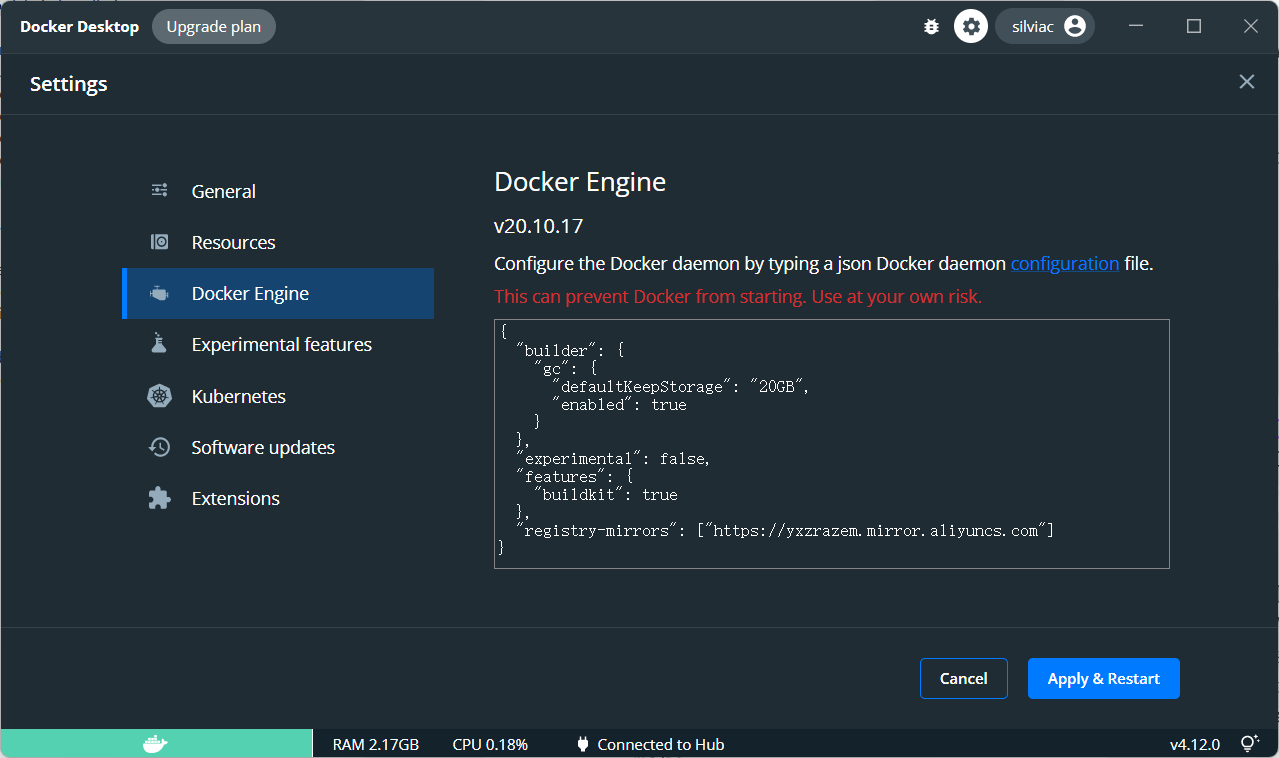
\includegraphics[width=\textwidth]{images/23.png}
\end{figure}
Remember to add a comma in the previous line for valid syntax. Then, apply and restart Docker Desktop. Wait until the Docker is started. Re-run \texttt{./build\_openroad.sh}.

\section{Design Compiler Reports}\label{ADC}
\subsection{Timing Report}
The correct timing report is:
\begin{minted}[breaklines,breakanywhere]{text}
Information: Updating design information... (UID-85)

****************************************
Report : timing
        -path full
        -delay max
        -nets
        -max_paths 1
        -transition_time
Design : SortUnitStructRTL__nbits_8
Version: R-2020.09-SP3
Date   : Sat Nov 12 20:50:16 2022
****************************************

Operating Conditions: typical   Library: NangateOpenCellLibrary
Wire Load Model Mode: top

  Startpoint: elm_S1S2__2/out_reg[1]
              (rising edge-triggered flip-flop clocked by ideal_clock1)
  Endpoint: elm_S2S3__0/out_reg[0]
            (rising edge-triggered flip-flop clocked by ideal_clock1)
  Path Group: ideal_clock1
  Path Type: max

  Des/Clust/Port     Wire Load Model       Library
  ------------------------------------------------
  SortUnitStructRTL__nbits_8 5K_hvratio_1_1 NangateOpenCellLibrary

Attributes:
    d - dont_touch
    u - dont_use
   mo - map_only
   so - size_only
    i - ideal_net or ideal_network
  inf - infeasible path

  Point                                       Fanout     Trans      Incr       Path      Attributes
  ---------------------------------------------------------------------------------------------------------
  clock ideal_clock1 (rise edge)                                    0.00       0.00

  elm_S1S2__2/out_reg[1]/CK (DFF_X1)                      0.00      0.00       0.00 r
  elm_S1S2__2/out_reg[1]/Q (DFF_X1)                       0.01      0.09       0.09 r
  elm_S1S2__2/out[1] (net)                      2                   0.00       0.09 r
  elm_S1S2__2/out[1] (Reg__Type_Bits8_6)                            0.00       0.09 r
  elm_S1S2__out[2][1] (net)                                         0.00       0.09 r
  minmax0_S2/in1[1] (MinMaxUnit__nbits_8_4)                         0.00       0.09 r
  minmax0_S2/in1[1] (net)                                           0.00       0.09 r
  minmax0_S2/U39/ZN (INV_X1)                              0.00      0.02       0.11 f
  minmax0_S2/n24 (net)                          1                   0.00       0.11 f
  minmax0_S2/U57/ZN (AOI21_X1)                            0.02      0.04       0.15 r
  minmax0_S2/n16 (net)                          1                   0.00       0.15 r
  minmax0_S2/U58/ZN (AOI222_X1)                           0.02      0.04       0.18 f
  minmax0_S2/n17 (net)                          1                   0.00       0.18 f
  minmax0_S2/U36/ZN (NOR3_X1)                             0.03      0.05       0.24 r
  minmax0_S2/n18 (net)                          1                   0.00       0.24 r
  minmax0_S2/U9/ZN (NOR3_X1)                              0.01      0.02       0.26 f
  minmax0_S2/n19 (net)                          1                   0.00       0.26 f
  minmax0_S2/U33/ZN (NOR3_X1)                             0.03      0.05       0.31 r
  minmax0_S2/n20 (net)                          1                   0.00       0.31 r
  minmax0_S2/U28/ZN (NOR3_X1)                             0.01      0.02       0.33 f
  minmax0_S2/n21 (net)                          1                   0.00       0.33 f
  minmax0_S2/U59/ZN (OAI22_X1)                            0.04      0.05       0.38 r
  minmax0_S2/n23 (net)                          2                   0.00       0.38 r
  minmax0_S2/U23/ZN (OAI21_X1)                            0.02      0.05       0.43 f
  minmax0_S2/N1 (net)                           2                   0.00       0.43 f
  minmax0_S2/U1/ZN (INV_X1)                               0.05      0.08       0.50 r
  minmax0_S2/n4 (net)                          10                   0.00       0.50 r
  minmax0_S2/U47/ZN (OAI22_X1)                            0.02      0.04       0.55 f
  minmax0_S2/out_min[0] (net)                   1                   0.00       0.55 f
  minmax0_S2/out_min[0] (MinMaxUnit__nbits_8_4)                     0.00       0.55 f
  minmax0_S2__out_min[0] (net)                                      0.00       0.55 f
  elm_S2S3__0/in_[0] (Reg__Type_Bits8_4)                            0.00       0.55 f
  elm_S2S3__0/in_[0] (net)                                          0.00       0.55 f
  elm_S2S3__0/out_reg[0]/D (DFF_X1)                       0.02      0.01       0.56 f
  data arrival time                                                            0.56

  clock ideal_clock1 (rise edge)                                    0.60       0.60
  clock network delay (ideal)                                       0.00       0.60

  library setup time                                               -0.04       0.56
  data required time                                                           0.56
  ---------------------------------------------------------------------------------------------------------
  data required time                                                           0.56
  data arrival time                                                           -0.56
  ---------------------------------------------------------------------------------------------------------
  slack (MET)                                                                  0.00

1
\end{minted}
\subsection{Area Report}
The correct area report is
\begin{minted}[breaklines,breakanywhere]{text}
****************************************
Report : area
Design : SortUnitStructRTL__nbits_8
Version: R-2020.09-SP3
Date   : Sat Nov 12 20:50:35 2022
****************************************

Library(s) Used:

    NangateOpenCellLibrary (File: /home/users/ece481/freepdk-45nm/stdcells.db)

Number of ports:                          466
Number of nets:                           849
Number of cells:                          458
Number of combinational cells:            339
Number of sequential cells:                99
Number of macros/black boxes:               0
Number of buf/inv:                        123
Number of references:                      22

Combinational area:                327.446005
Buf/Inv area:                       74.214000
Noncombinational area:             447.677984
Macro/Black Box area:                0.000000
Net Interconnect area:      undefined  (Wire load has zero net area)

Total cell area:                   775.123989
Total area:                 undefined

Hierarchical area distribution
------------------------------

                                  Global cell area          Local cell area
                                  ------------------  ---------------------------
Hierarchical cell                 Absolute   Percent  Combi-    Noncombi-  Black-
                                  Total      Total    national  national   boxes   Design
--------------------------------  ---------  -------  --------  ---------  ------  -----------------------------------
  SortUnitStructRTL__nbits_8
elm_S0S1__0                         36.1760      4.7    0.0000    36.1760  0.0000  Reg__Type_Bits8_0
elm_S0S1__1                         36.1760      4.7    0.0000    36.1760  0.0000  Reg__Type_Bits8_11
elm_S0S1__2                         36.1760      4.7    0.0000    36.1760  0.0000  Reg__Type_Bits8_10
elm_S0S1__3                         36.1760      4.7    0.0000    36.1760  0.0000  Reg__Type_Bits8_9
elm_S1S2__0                         36.1760      4.7    0.0000    36.1760  0.0000  Reg__Type_Bits8_8
elm_S1S2__1                         36.1760      4.7    0.0000    36.1760  0.0000  Reg__Type_Bits8_7
elm_S1S2__2                         36.1760      4.7    0.0000    36.1760  0.0000  Reg__Type_Bits8_6
elm_S1S2__3                         36.1760      4.7    0.0000    36.1760  0.0000  Reg__Type_Bits8_5
elm_S2S3__0                         36.1760      4.7    0.0000    36.1760  0.0000  Reg__Type_Bits8_4
elm_S2S3__1                         36.1760      4.7    0.0000    36.1760  0.0000  Reg__Type_Bits8_3
elm_S2S3__2                         36.1760      4.7    0.0000    36.1760  0.0000  Reg__Type_Bits8_2
elm_S2S3__3                         36.1760      4.7    0.0000    36.1760  0.0000  Reg__Type_Bits8_1
minmax0_S1                          56.3920      7.3   56.3920     0.0000  0.0000  MinMaxUnit__nbits_8_0
minmax0_S2                          56.6580      7.3   56.6580     0.0000  0.0000  MinMaxUnit__nbits_8_4
minmax1_S1                          55.5940      7.2   55.5940     0.0000  0.0000  MinMaxUnit__nbits_8_3
minmax1_S2                          58.5200      7.5   58.5200     0.0000  0.0000  MinMaxUnit__nbits_8_2
minmax_S3                           59.0520      7.6   59.0520     0.0000  0.0000  MinMaxUnit__nbits_8_1
val_S0S1                             5.8520      0.8    1.3300     4.5220  0.0000  RegRst__Type_Bits1__reset_value_0_0
val_S1S2                             5.8520      0.8    1.3300     4.5220  0.0000  RegRst__Type_Bits1__reset_value_0_2
val_S2S3                             5.8520      0.8    1.3300     4.5220  0.0000  RegRst__Type_Bits1__reset_value_0_1
--------------------------------  ---------  -------  --------  ---------  ------  -----------------------------------
Total                                                 327.4460   447.6780  0.0000

1
\end{minted}

\section{Change Log}
Fall 2022: Yihua Liu
\begin{itemize}
    \item created this lab
\end{itemize}

\printbibliography

\end{document}
